\documentclass{article}
\usepackage[
    left=1.5in, 
    right=1in, 
    top=1in,
    top=1in]{geometry}
\usepackage{blindtext}
\usepackage{graphicx}

\usepackage{amsfonts}
\usepackage{amsmath}
\usepackage{amsthm}
\usepackage{float}
\usepackage{graphicx}
\usepackage{hyperref}
\usepackage{bbm}
\usepackage{algorithm}
\usepackage[noend]{algpseudocode}
\usepackage{courier}
\usepackage{setspace}

\newtheorem{theorem}{Theorem}[section]
\newtheorem{corollary}{Corollary}[theorem]
\newtheorem{lemma}[theorem]{Lemma}

\makeatletter
\def\BState{\State\hskip-\ALG@thistlm}
\makeatother

% correct bad hyphenation here
\begin{document}
\title{Upon the Deanonymization of Bitcoin Transactions}
\author{Yash Patel, Matt Weinberg}

\begin{center}
\thispagestyle{empty}
\parskip=14pt%
\vspace*{5\parskip}%
\LARGE{DEANONYMIZING BITCOIN TRANSACTIONS} \\
\large{AN INVESTIGATIVE STUDY ON LARGE-SCALE GRAPH CLUSTERING}

\vspace*{5\parskip}%
\large{A senior thesis \\
submitted to the Department of Mathematics \\
in partial fulfillment of the requirements for \\
the degree of Bachelor of Arts}

\vspace*{4\parskip}%
By

Yash Patel

\rule{7cm}{0.4pt}\\
Under the supervision of

S. Matthew Weinberg

Princeton University\\
Princeton, New Jersey

May 7, 2018
\end{center}
\clearpage

\doublespacing
\section*{Acknowledgements}
\pagenumbering{roman}I would like to extend a profound thank you to the following people involved directly or indirectly in the writing of my thesis:

My thesis advisor for having spent countless hours explaining and re-explaining the relevant concepts for my research work, for helping guide me through the foreign land of research material for my junior IW and senior thesis alike, and for always being a motivated and enthusiastic voice to bounce ideas off of for bringing the project forward.

My parents for having constantly pushed me forward and supported me on my journey through my academic challenges at Princeton and onward into the future.

My sister for having been the best friend a brother could wish for, always reminding me to see the bright side of any situation as it comes. 

My friends from Quad, Naacho, and the Princeton community at large, who always managed to turn every moment, from the most light to the most stressful, into a greatly memorable experience.

\clearpage
\singlespacing
\tableofcontents
\clearpage
\listoffigures
\listoftables
\clearpage

\begin{abstract}
Bitcoin has emerged from the fringes of technology to the mainstream investment public recently. With speculation rampant, Bitcoin has become more and more the subject of harsh criticism in ascertaining its use case. Unfortunately, much of Bitcoin's present use case is for transactions in online black markets. Towards that end, various studies have sought to partially deanonymize Bitcoin transactions, identifying wallets associated with major players in the space to help forensic analysis and to taint wallets involved with criminal activity. Relevant past studies, however, have rigidly enforced manually constructed heuristics to perform such deanonymization, paralleling an extensive union-find algorithm. We wish to extend this work by introducing many more heuristics than were previously considered and performing a graph clustering on this extensive ``heuristics graph." Towards that end, we explored the performance of various spectral, k-means, and METIS clustering algorithms on the SBM (stochastic block model) as a prototype of the heuristics graph and found hierarchical spectral clustering and METIS to have the best performance by the standard purity, NMI, and F-score clustering accuracy metrics. METIS was subsequently employed to be applied to the full graph due to major time concerns with the hierarchical spectral clustering, from which patterns of online use were extracted and confirmed with a known ground truth set. Future extensions of this work should seek to refine the hierarchical spectral clustering algorithm for its time deficiencies and refine METIS in regimes of high spatial separability.
\end{abstract}

\clearpage
\pagenumbering{arabic}
\doublespacing
\section{Introduction}
Bitcoin (BTC), previously relegated as a technology for only the most technologically competent of computer scientists, has emerged into the mainstream public in an enormous way. Ever since its explosive rise over the past year, technologists and investors both have sought to understand and exploit its technical possibilities. As illustrated in Figure \ref{fig:BTC_price}, speculation on Bitcoin, both directly and in the form of associated ETF derivative markets \cite{bitcoin-etf}, has become an undeniable sector of the modern technology world. While current speculations are high, many investors and technologists alike struggle to understand the fundamental use case of Bitcoin and its underlying technology: blockchain. The speculative bubble is largely the product of vacuous interest pooling into an asset of misunderstood potential, paralleling the financial situation surrounding the dot-com bubble. 

\begin{figure}[H]
    \centering
    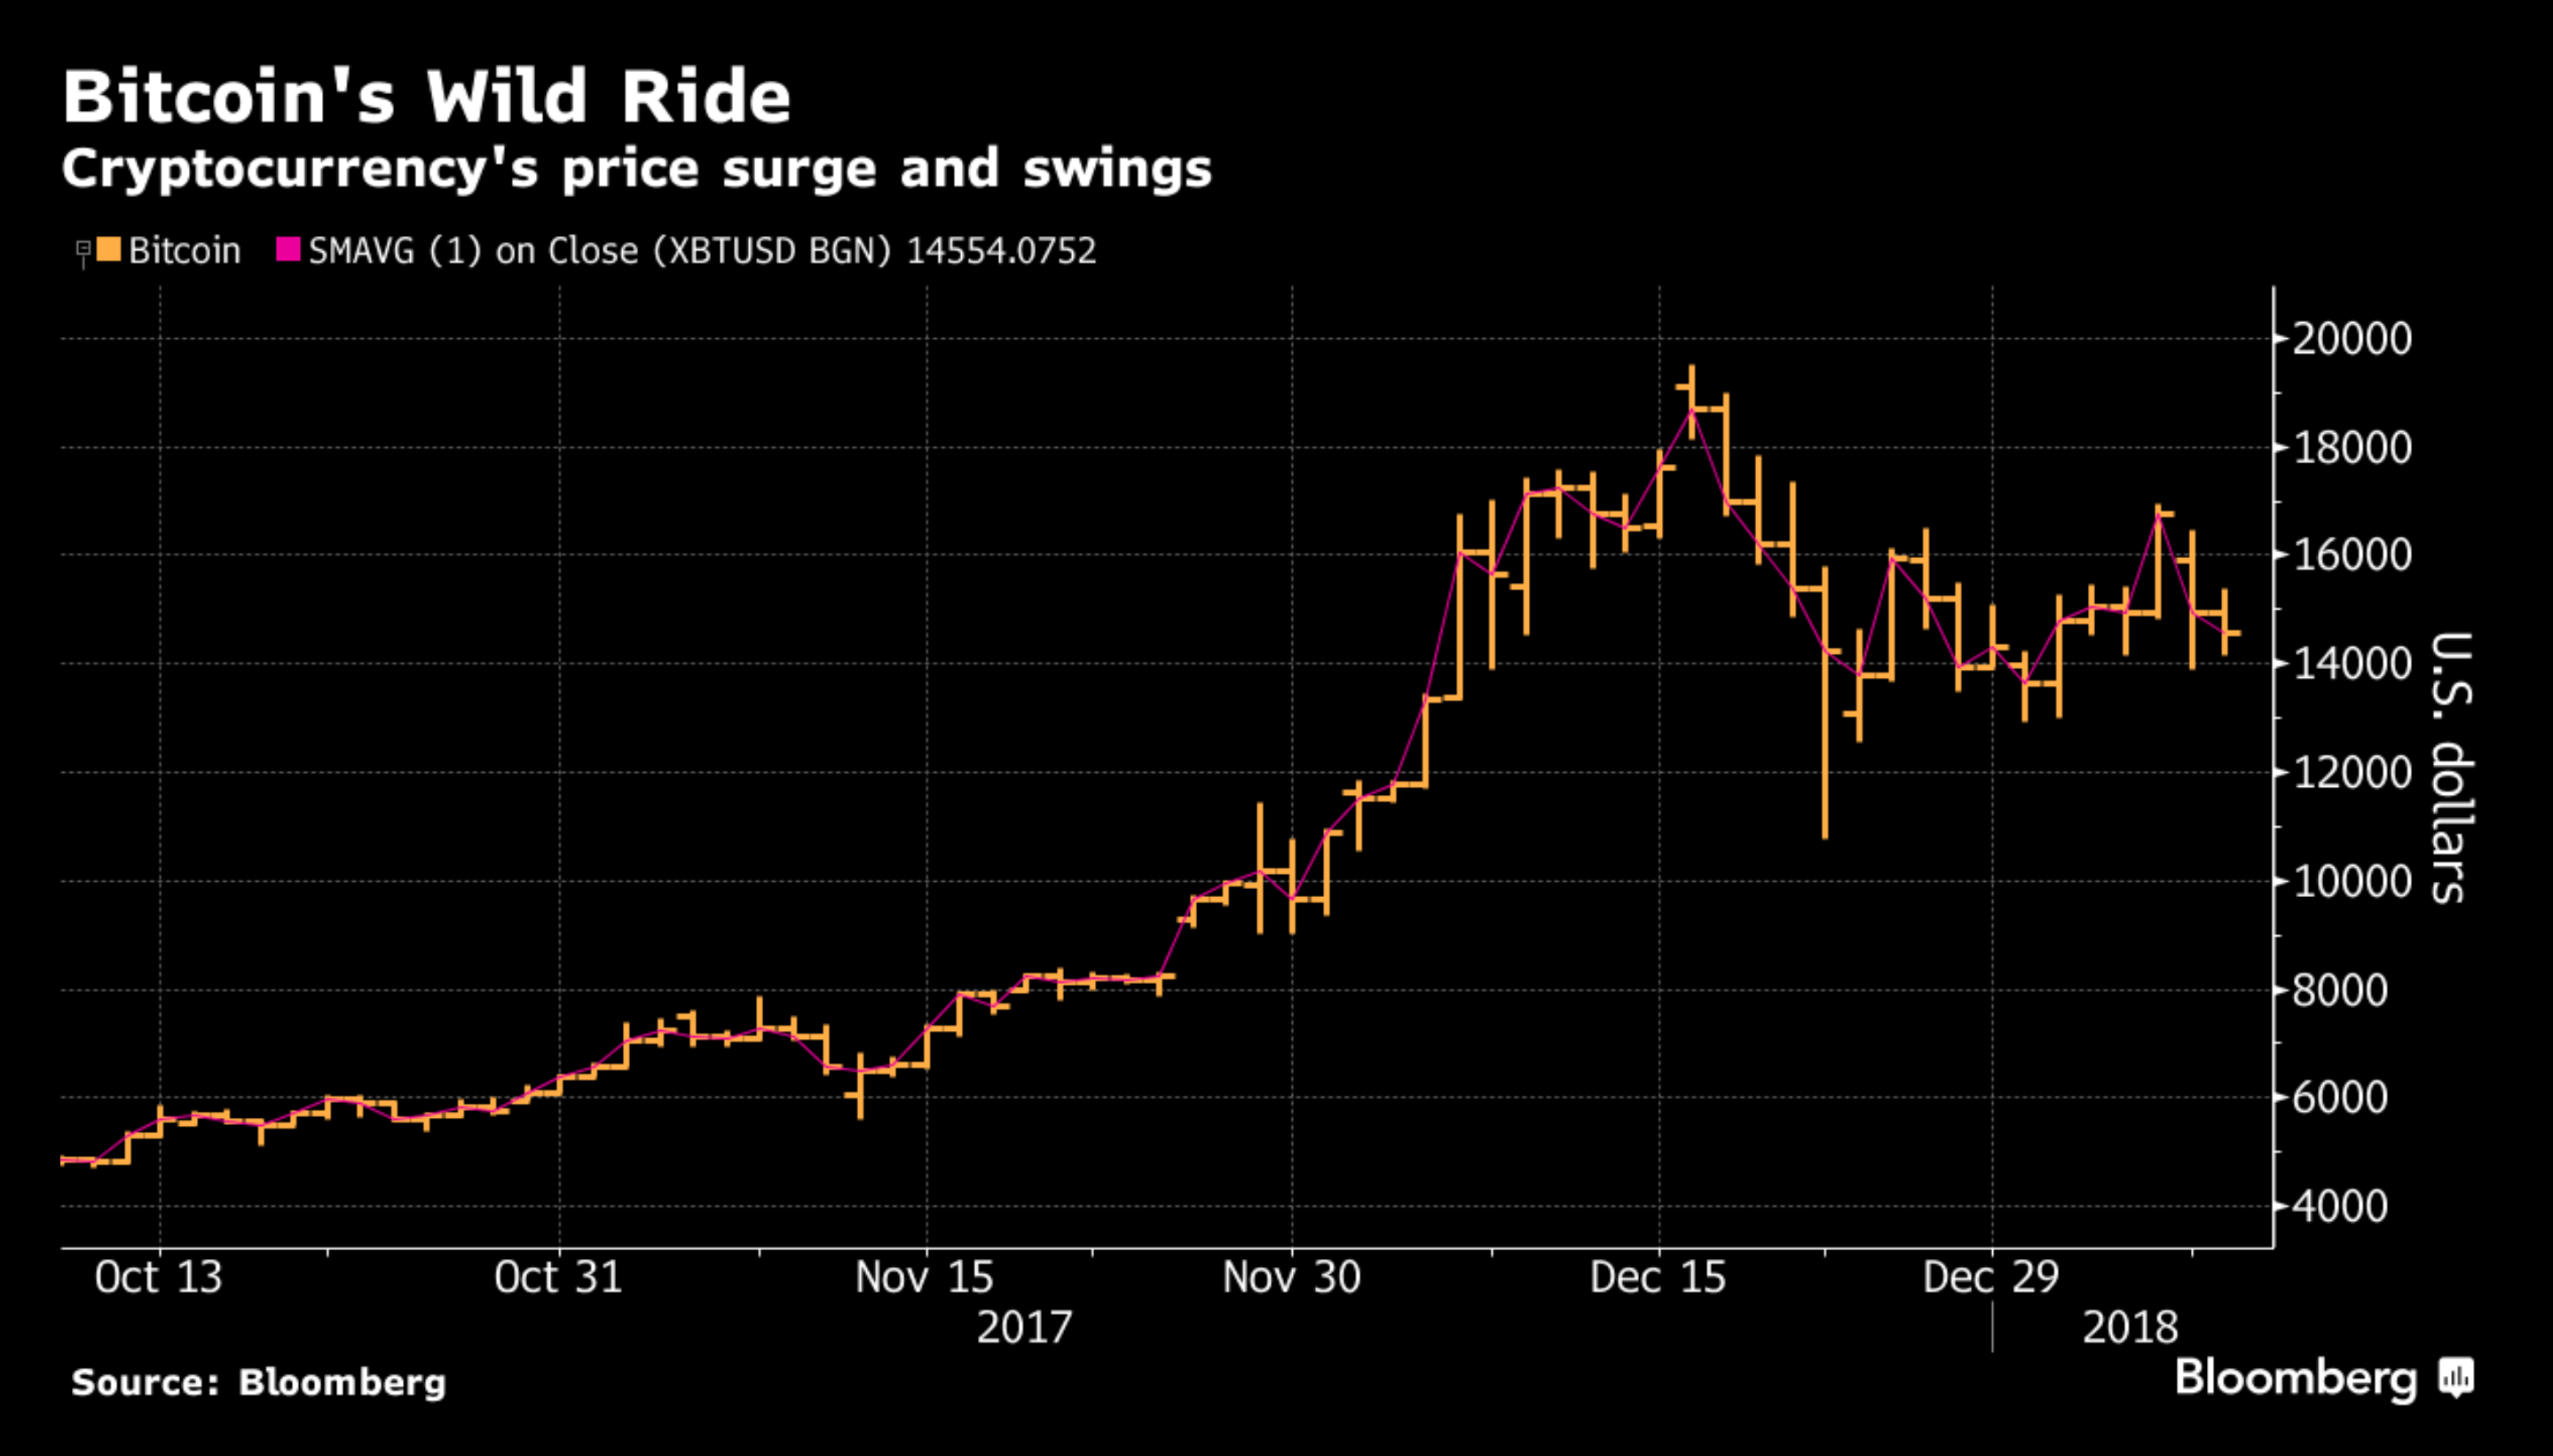
\includegraphics[width=.50\textwidth]{BTC_price.png}
    \caption[Bitcoin Price]{The price of one Bitcoin, as tracked by Bloomberg. While technologists saw its promise many years prior, Bitcoin's rise in popularity in the general public has led to exponential speculative interest recently \cite{goldman}.}
    \label{fig:BTC_price}
\end{figure}

Prior to further discussing Bitcoin's use cases as a whole, it serves a purpose to understand the underlying technology first. Briefly, Bitcoin is a cryptocurrency, by which we mean a ``digital unit of exchange that is not backed by a government-issued legal tender" \cite{virtual}. The blockchain technology underpinning Bitcoin and other cryptocurrencies, as illustrated in Figure \ref{fig:blockchain}, is ``a solution to the double-spending problem using a peer-to-peer distributed timestamp server to generate computational proof of the chronological order of transactions. The system is secure as long as honest nodes collectively control more CPU power than any cooperating group of attacker nodes" \cite{bitcoin}. Described plainly, blockchain seeks to solve a technical problem, namely that of achieving consensus in a distributed system, i.e. to arbitrate exchange of a common asset without the need of a trusted central authority. Since the desired end goal is transactions without a trusted third-party, it must be the case that any peer in this network can verify transactions as valid. This circumstance lends itself naturally to the well-known concept of public-key encryption. It, therefore, should come as little surprise that this is how wallets are implemented in Bitcoin and similar cryptocurrencies.

Specifically, as with any public-key encryption system, Bitcoin exchange revolves around participating members having two keys, one public and one private. For the specific use case of Bitcoin, the private key is used to sign any transactions messages being made to another wallet. In turn, any other account, particularly that of a receiving party, can verify it indeed originated from the claimed party using the public key, as demonstrated in further detail in Figure \ref{fig:address}.

\begin{figure}
    \centering
    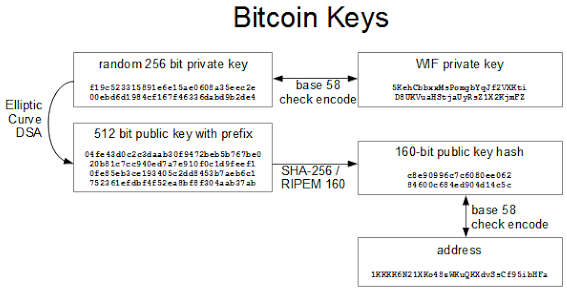
\includegraphics[width=.75\textwidth]{address.png}
    \caption[Bitcoin Public-Key Wallets]{While public-key encryption is the basic idea behind the Bitcoin protocol, there are many additional details involved in making it a practical system to be used. In particular, additional hashing functions are used in an effort to make the underlying keys more manageable to deal with and store as an end user, while meeting sufficient security demands. These details, while interesting in their own right, however, are not of key important for this particular study \cite{public-key}.}
    \label{fig:address}
\end{figure}

Incidentally, these public keys serve as what people colloquially refer to as their ``wallets." Specifically, ``Bitcoin\dots is designed with pseudonymous identities. Account numbers are public keys of a specific asymmetric encryption system" \cite{laundering}. This notion of Bitcoin being ``pseudonymous" refers to the presence of an abstraction layer between real life and those IDs used within the Bitcoin universe, despite the Bitcoin IDs and their associated activities being publicly visible. In a fully anonymous protocol, there would be no information revealed in public channels.

\begin{figure}
    \centering
    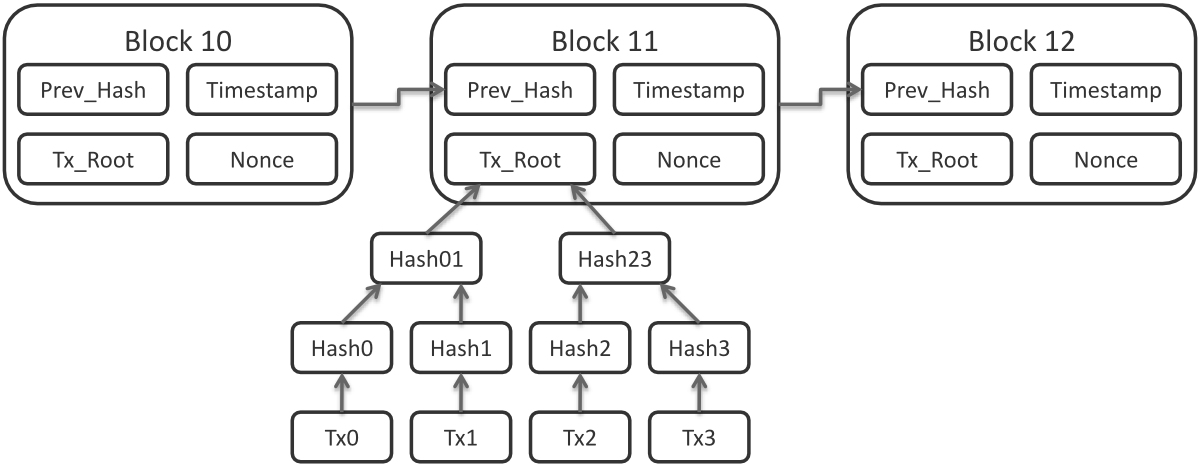
\includegraphics[width=.75\textwidth]{blockchain.png}
    \caption[Blockchain Data Structure]{Blockchain, the underlying technology behind Bitcoin and all other cryptocurrencies, is simply a data structure consisting of an extended linked list of hash pointers with metadata. These pieces of metadata, in addition to carrying the actual BTC transaction information, more importantly serve data that can be used for efficient verification of double-spending in a distributed system \cite{blockchain-img}.}
    \label{fig:blockchain}
\end{figure}

Returning to the discussion of interest, Bitcoin, when viewed from this perspective, has no properties making it inherently more conducive to privacy aside from the abstraction of people's connection to their public wallet addresses. This abstraction, in fact, is seemingly fully comparable to that imposed by the current banking system abstracting a person's account number from his real life identity. The key differences, however, are twofold. In the first place, the abstraction layer instituted by banks are leaky. That is to say, while people generally do not know one another's account numbers, authorities within banks have this association, for they always require personal details be provided in signing up for an account by the famous ``know your customer" adage. Bitcoin has no similar gatekeeper with such identifying information by virtue it being a trustless protocol, meaning Bitcoin wallets can be procured without the need to link them to personal details. The second distinguishing feature is the ease with which such wallets can be created. In line with the lack of a central authority, there is no barrier in place preventing a single person or entity from creating many Bitcoin wallets. This follows as, in the process of making a wallet, there is \textit{no} way to distinguish whether the creator is someone who has made a wallet or not due to the lack of associated identifying attributes. Thus, the properties of privacy that have come to be associated with Bitcoin have been born out of its lack of a central authority holding identifying links. 

Returning to the discussion of the use cases of Bitcoin, many have been born out of this seeming impossibility in linking real-life identity with associated transaction wallets. It, therefore, seems natural that such use cases are generally of some illicit nature, as, if they were not, there would be no benefit of using Bitcoin over a traditional bank, as the former does not provide the typical fraud protections that are instituted by the latter. One government report discussed cryptocurrencies in the following light:

``[Cryptocurrencies] present particularly difficult law enforcement challenges because of their ability to transcend national borders in the fraction of a second, unique jurisdictional issues and anonymity due to encryption. Due primarily to their anonymity, virtual currencies have been linked to numerous types of crimes, including facilitating marketplaces for: assassins, attacks on businesses, the exploitation of children (including pornography), corporate espionage, counterfeit currencies, drugs, fake IDs and passports, high yield investment schemes (Ponzi schemes and other financial frauds), sexual exploitation, stolen credit cards and credit card numbers, and weapons" \cite{virtual}. 

To point to one particular example, the Silk Road, an ``online market...[that] specialized in `black market' goods, such as pornography, weapons or narcotics...corresponded to about 4.5\% of all transactions occurring in exchange" during the early days of Bitcoin \cite{silk}. While Bitcoin's integration into the mainstream has greatly exploded since these statistics were measured, the fact remains that a significant portion of Bitcoin's trading activity lie in either illicit or speculation markets. It, therefore, becomes a question of interest whether such illicit activity can be tracked and retraced. By this, we mean to say, produce a map that links wallet addresses to real-life identities. What is meant by ``real-life identities" is somewhat ill-defined, as to what level of granularity we wish to resolve. For example, a group of addresses could be resolved as ``John Smith" or ``Coinbase" assuming John Smith has his wallet handled through Coinbase. 

Briefly, Coinbase is a platform employed by many BTC users that performs two primary purposes: serving as a platform of exchange for cryptocurrencies from traditional currencies and providing a simple way to set up wallets. These wallets, however, are not ``owned" by the end user in the traditional sense; the private key is owned by Coinbase. Internally, they simply have a map linking a particular private key to the user's account, meaning any activity desired by the user on Coinbase is simply relayed to the Coinbase API, which serves as a ``middleman" to the end Bitcoin application layer. The main takeaway is that Coinbase serves as a central manager of the accounts of many end users, making it a clear target for deanonymization, as we further expound upon in Section \ref{background}.

Thus, the main objective of the study herein was to deanonymize Bitcoin transacations to as great an extent as possible, as conveyed upon above. The outline of this paper is as follows:
\begin{itemize}
    \item \textbf{Section \ref{background}:} Covers through the major technical topics of interest that are to be used in the remainder of the paper. Most of the findings presented through this section entail a literature review of well-known works in their respective fields, although occasional novel material is presented when appropriate for sake of organization. We further note that a majority of figures presented through this section entail those catered from previous research endeavors.
    \item \textbf{Section \ref{methodology}:} Walks through the structure of the experiments that were written and conducted. The code is freely available at: \url{https://github.com/yashpatel5400/anonychain}. We also provide the specifics of the expected structure of results from each experiment.
    \item \textbf{Section \ref{results}:} Presents the results of the experiments laid of in the previous section, all in the form of relevant visualizations.
    \item \textbf{Section \ref{discussion}:} Discusses the main takeaways from the graphical results as they relate to the research problem posed above. Specifically, these discussions pointedly answer the extent to which various clustering techniques can be used for deanonymizing Bitcoin transactions.
    \item \textbf{Section \ref{conclusion}:} Provide follow-up research ideas that could be pursued should readers feel inspired and interested in furthering the research conducted herein.
\end{itemize}

\clearpage
\section{Background}\label{background}
To follow is the necessary technical background for the paper, of which a majority concentrates on material from graph theory. We begin by presenting the current state-of-the-art in this deanonymization space and subsequently discuss all relevant technical concepts as they relate to this study. 

\subsection{Deanonymization Techniques}
Currently, two main studies have come to define the space of deanonymization, whose results and limitations we discuss herein. The objective of both was exactly that we have for this study, presented as ``our goal is not to generally deanonymize all Bitcoin users - as the abstract protocol design itself dictates that this should be impossible - but rather to identify certain idioms of use present in concrete Bitcoin network implementations that erode the anonymity of the users who engage in them" \cite{fistful}. In other words, there is no way to go from the raw BTC address information to a real-world identity. However, as with any practical system, there are often leaks in information due to sheer negligence by the end user. This parallels how, despite there being many supposed ``hacks" of Yahoo mail, this has little to do with the encryption of their internal systems, but rather due to the laziness of end users in procuring difficult-to-guess passwords.

In a similar fashion, end users often reveal information intended to be kept private in public channels. For example, people may post their wallet addresses on online forums, from which a link between the address and a real-world entity can be established. By exploiting such side-channel leaked information, we can gather a base set of truth regarding who owns a particular wallet, i.e. catering a list saying that address 1Mz7153HMuxXTuR2R1t78mGSdzaAtNbBWX is owned by John Doe and so on. This list, however, will be a very tiny subset of the addresses produced on the BTC network. It is, therefore, the objective herein to expand from this tiny seed of base information to determine the identities of as many other wallets as possible. While seemingly of little use, the purpose of this becomes clear in remembering that many people own multiple BTC wallets. In other words, John Doe, from the previous example, may own three other wallets other than 1Mz7153HMuxXTuR2R1t78mGSdzaAtNbBWX. Having tainted his privacy with this public information leak, it is our objective, therefore, to associate these other three wallet IDs with his name.

Of course, while gathering a comprehensive ground truth is critical for deanonymizing as great a proportion of the network as possible, we similarly consider it useful to cluster sets of wallets as being owned by a single entity. When any one of these wallets has a public side-channel leak in the future, therefore, this information can be retroactively applied onto the clustering, from which the identities of a series of other wallets too become revealed. Thus, the act of grouping wallets as being owned by a single entity is effectively the goal of this study, for which we use the procured ground truth as a method of verification. Once again, the specifics of this procedure are elaborated in Section \ref{methodology}.

An example as told by the authors of this study is as follows: ``This clustering allows us to amplify the results of our re-identification attack: if we labeled one public key as belonging to Mt. Gox, we can now transitively taint the entire cluster containing this public key as belonging to Mt. Gox as well" \cite{fistful}. For context, Mt. Gox served a very similar role to that which Coinbase currently fills. It should therefore be clear why they ``consider de-anonymization of Bitcoin addresses as a clustering problem...Bitcoin address clustering is fairly different from classical clustering problems as there is no direct information about the objects' (addresses) such as coordinates or distances. The other peculiarity of the problem is the vastness of the Bitcoin blockchain, which requires designing computationally efficient algorithms for its' clustering" \cite{automatic}. In other words, there are two problems at hand that require solving. 

The first is determining and procuring a weighted graph with the property that if the edge connecting two vertices $v_{A},v_{B}$ has an associated weight we denote as $w_{AB}$ and satisfies $w_{AB} > w_{BC}$, there is a higher likelihood that the wallets associated with vertices $A,B$ indeed correspond to the same real-world entity as compared to that for $B,C$. The second problem is that of developing or discerning which clustering algorithms are capable at running at this scale within reasonable accuracy and time bounds.

We begin by discussing the first issue at hand. While it may seem natural to simply make use of the transaction ($tx$) history, seeing as there is a clear canonical mapping from this transaction to a weighted graph, it becomes clear that two accounts having many transactions between them has no bearing on them being the same entity. After all, if account $A$ has many transactions with account $B$, there is no reason to believe they correspond to the same \textit{or} different people. To rephrase, we wish to procure a graph that is built atop the raw transactions with a series of heuristics, some of which have arisen from the the paper being discussed.

Prior to discussing this heuristic, we introduce the notion of a change address. ``Change addresses are the mechanism used to give back to the input user in a transaction, as Bitcoins can be divided only by being spent" \cite{fistful}. In other words, the Bitcoin protocol prevents an account that owns 10 BTC from only sending five of its BTC to another account. Instead, the account must spend the entirety of the 10 BTC, with five going to the desired recipient and the other five to a ``change address" owned by the original owner though this change address may simply be the original wallet. Having said that, we can discuss the two heuristics used previously for linking addresses.

\begin{theorem}
``If two (or more) addresses are inputs to the same transaction, they are controlled by the same user; i.e., for any transaction $t$, all $pk\in\text{inputs}(t)$  are controlled by the same user" \cite{fistful}.
\end{theorem}

The main idea behind this is that all the inputs of a given transaction must sign off the transaction with their private key. We assume that end users are not sharing their private keys, for revealing such information essentially gives the recipient full authority of the associated account, in terms of being able to send any BTC held in the account. Thus, as \textit{all} input accounts must sign off the transaction, all the private keys must be at present simultaneously to validate the transaction, which can only happen if a single real-world entity knows the private keys of all the associated accounts. This heuristic is likely the most trustworthy of the ones considered, meaning its percent of false positives is extremely low. 

While this is the case, this heuristic is not remotely comprehensive. That is to say, there are \textit{many} more wallets that are owned by the same entity as compared to those that appear together as inputs in a single transaction. Thus, it is of interest to present other heuristics that may have a lower robustness but still contains some information regarding the likelihood of wallets corresponding to the same real-world entity. The second heuristic presented from the paper was as follows:

\begin{theorem}
``The  one-time  change  address  is  controlled  by the same user as the input addresses; i.e., for any transaction $t$,the controller of $\text{inputs}(t)$ also controls the one-time change address $pk \text{outputs}(t)$ (if such an address exists)" \cite{fistful}.
\end{theorem}

In other words, we expect that change addresses, when identifiable as such, are controlled by the originator of the transaction. To identify change addresses, the following intuition was followed: ``Working off the assumption that a change address has only one input (again,  as it is potentially unknown to its owner and is not re-used by the client), we first looked at the outputs of every transaction. If only one of the outputs met this pattern, then we identified that output as the change address. If, however, multiple outputs had only one input and thus the change address was ambiguous, we did not label any change address for that transaction" \cite{fistful}.

Thus, ``A Fistful of Bitcoins" procured a clustering by directly applying the two heuristics on the raw transaction graph to produce \ref{fig:fistful}. The paper, however, faced many issues issues related to directly clustering the graph as defined by these two heuristics. The primary of which was ``falsely linking even a small number of change addresses might collapse the entire graph into large `super-clusters' that are not actually controlled by a single user" \cite{fistful}. With that in mind, we catered heuristics that tended towards favoring false negatives as compared to false positives with the idea that the latter would result in clustering with little sematic value. In fact, the original iteration of their clustering ``ended up with a giant super-cluster containing the public keys of Mt. Gox, Instawallet, BitPay, and Silk Road, among others" \cite{fistful}. It was only after refining the second heuristic that this issue was resolved and there were distinct clusters formed. 

\begin{figure}
    \centering
    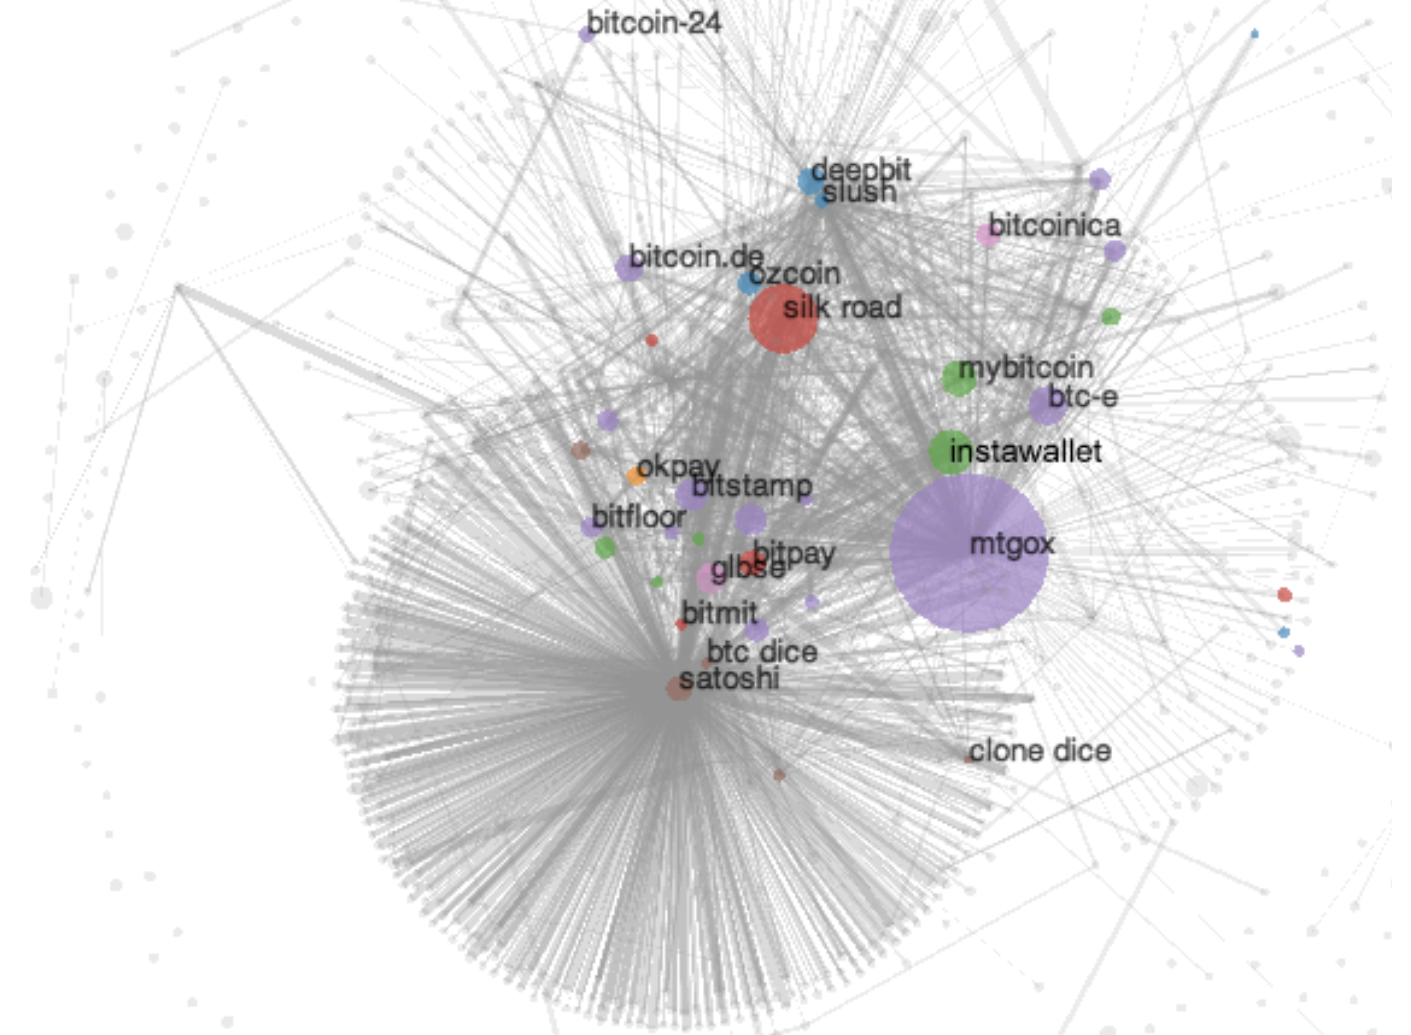
\includegraphics[width=.75\textwidth]{fistful.png}
    \caption[``Fistful of Bitcoins" Result]{The deanonymization results from ``A Fistful of Bitcoins." This clearly demonstrates that, using careful catered heuristics and large-scale graph clustering, certain portions of the network can be identified with high levels of confidence. The goal of this investigation, therefore, was to procure a graph similar in nature with an even greater number of addresses identified \cite{fistful}.}
    \label{fig:fistful}
\end{figure}

As discussed in the paper itself, there were a few limitations of this investigation, some of which we sought to rectify herein. One such limitation was that ``our new clustering heuristic is not fully robust in the face of changing behavior,\dots[i.e. in the face of] the gap [between actual and potential anonymity evolving] over time, and what users do to achieve stronger anonymity guarantee" \cite{fistful}. One key limitation, therefore, is how these two heuristics have assumptions that fail to hold under some of the new anonymity services that have emerged atop the BTC network, such as BTC mixing.

These mixing services, also referred to as BTC tumblers, effectively mix up the input addresses to a new set of output wallets. In other words, mixing services act as trusted third parties, whereby participating members can transfer their funds to this trusted service wallet. The tumbler then distributes the money amongst three new wallets, which then randomly get assigned to the participating members. Of course, the value associated with the accounts involved in the mixing must be identical, else the owner of the accounts would be traceable through the mixing service. Assuming no collusion between the owner of the mixing service and any interested third parties, identities cannot directly be traced between the input and output addresses. The heuristics catered and discussed above, therefore, are unable to link addresses that have passed through such mixing services, since no pair of such addresses would appear in any connected transaction in the ways necessitated to form a link. This follows as it was the end user's intention in using the mixing service to disassociate the output from the input address, making it highly unlikely he would use the two in tandom in the future.

While this is the case, assuming the end user has some static characteristics, such as making transactions at only certain times of day or to only particular accounts, the original and mixed addresses should still be linkable, marking a clear deficiency in the heuristics catered above. We, therefore, sought to integrate a broader scope of heuristics to produce potential links between accounts. Of course, with this expanding set of heuristics arises the issue brought up within the ``Fistful of Bitcoins" paper, namely that of procuring a series of false positives that ultimately collapse the overall graph into a small number of superclusters. We delve further in depth as to particular methods employed to avoid said issue, but the main strategy revolves around another shortcoming of the approach employed by their clustering effort.

In particular, the heuristics they catered were rigidly employed, meaning their involvement in clustering was completely binary. That is to say, if heuristic 1 was satisfied for a pair of vertices, the two were clumped together as being the same entity immediately and similarly for heuristic 2. This rigidness was the source of the collapse and resulted in the need to make refinements on the second heuristic. We wished to produce a means by which the heuristics can be procured and make the system flexible so that it can automatically determine how effective the different heuristics are at linking two real-world entities and appropriately assign corresponding weights. That is to say, rather than having a binary means of clustering addresses, we wished to expand to a continuous space. 

The second main study in the realm of deanonymization, in fact, attempted to expand along these lines. It specifically produced a probabilistic model that describes the probability two vertices in their graph correspond to the same real-world entity, where the graph contains data both from the on-chain heuristics and off-chain information. Examples of the former are exactly those from the ``Fistful of Bitcoins" investigation whereas the latter are metadata associated with accounts of a particular entity. For example, ``Satoshi Bones Casino uses 1change and 1bones prefixes and BTC-E exchange uses 1eEUR and 1eUSD prefixes" \cite{automatic}. With the addition of this additional metadata ``heuristic," however, came additional noise in the sense that there are plenty examples thereof that do not indicate the end-user is in fact the same. As discussed in their paper, ``mostly informationless suffixes  (for example, .com, .co, @gmail)" were ignored \cite{automatic}. 

Towards that end, unlike the Fistful paper, the authors sought to procure a probabilistic model that effectively weighs the different heuristics based on their levels of confidence therein. In their words, their ``proposed  model  is  not  intended  to  capture the probabilistic structure of the real world, but more to give an  approach  for  systematical  study  of  confidence  trade-offs between different sources of information" \cite{automatic}. This is similar in nature to the approach employed herein. However, their weights were manually tuned by the researchers such that the eventual graph collapse aligned with expected ground truths. Our investigation sought to perform such tuning automatically, in a manner that parallels modern machine learning algorithms, specifically neural networks. In addition, we considered several additional heuristics of the off-chain nature described in their paper.

All in all, the current degree to which deanonymization has been accomplished demonstrates it is in fact a viable route of investigation. Yet, their limitations point to a gap in the heuristics hereto employed, specifically regarding the rigidity with which they were used in clustering.

\subsection{Data Procurement}
As discussed in the previous section, it follows that two pieces of data needed to be procured for this investigation, the first being the ground truth against which perfomance of the deanonymization could be checked and the second the heuristics graph on which the clustering would be performed. For the purposes of this investigation, the gap laid by the former was filled with the ground truth gratefully provided by the authors of the Fistful of Bitcoins paper. As for the latter, however, another relevant investigation was conducted, from which a tool dubbed ``Blocksci" was produced. Blocksci was born out of a need to perform analysis on public blockchain data. Per Blocksci's paper, ``Bitcoin's blockchain alone is 140 GB as of August 2017, and growing quickly. This data holds the key to measuring the privacy of cryptocurrencies in practice...Blocksci is 15x-600x faster than existing tools [and] comes bundled with analytic modules" \cite{blocksci}. In particular, Blocksci fills the void of being able to iterate through the entire blockchain of transactions, allowing for heuristics to be catered effectively in an online setting. That is to say, unlike heuristics procured in previous investigations, a heuristic could be procured in a reasonable timeframe by employing Blocksci, allowing greater flexibility in their curation. Thus, one of the main bottlenecks in procuring more heuristics was eliminated through the development of Blocksci.

While specific details of its internal implementation are not greatly of relevance to this investigation, we present some to make clear the process by which heuristics are produced. This is more clearly elaborated upon in Figure \ref{fig:blocksci}. Specifically, ``BlockSci's design starts with the observation that blockchains are append-only databases; further, the snapshots used for research are static. Thus, the ACID properties of transactional databases are unnecessary" \cite{blocksci}. In other words, by eliminating the unnecessary portions of database API, they streamlined the interface to end users. 

\begin{figure}
    \centering
    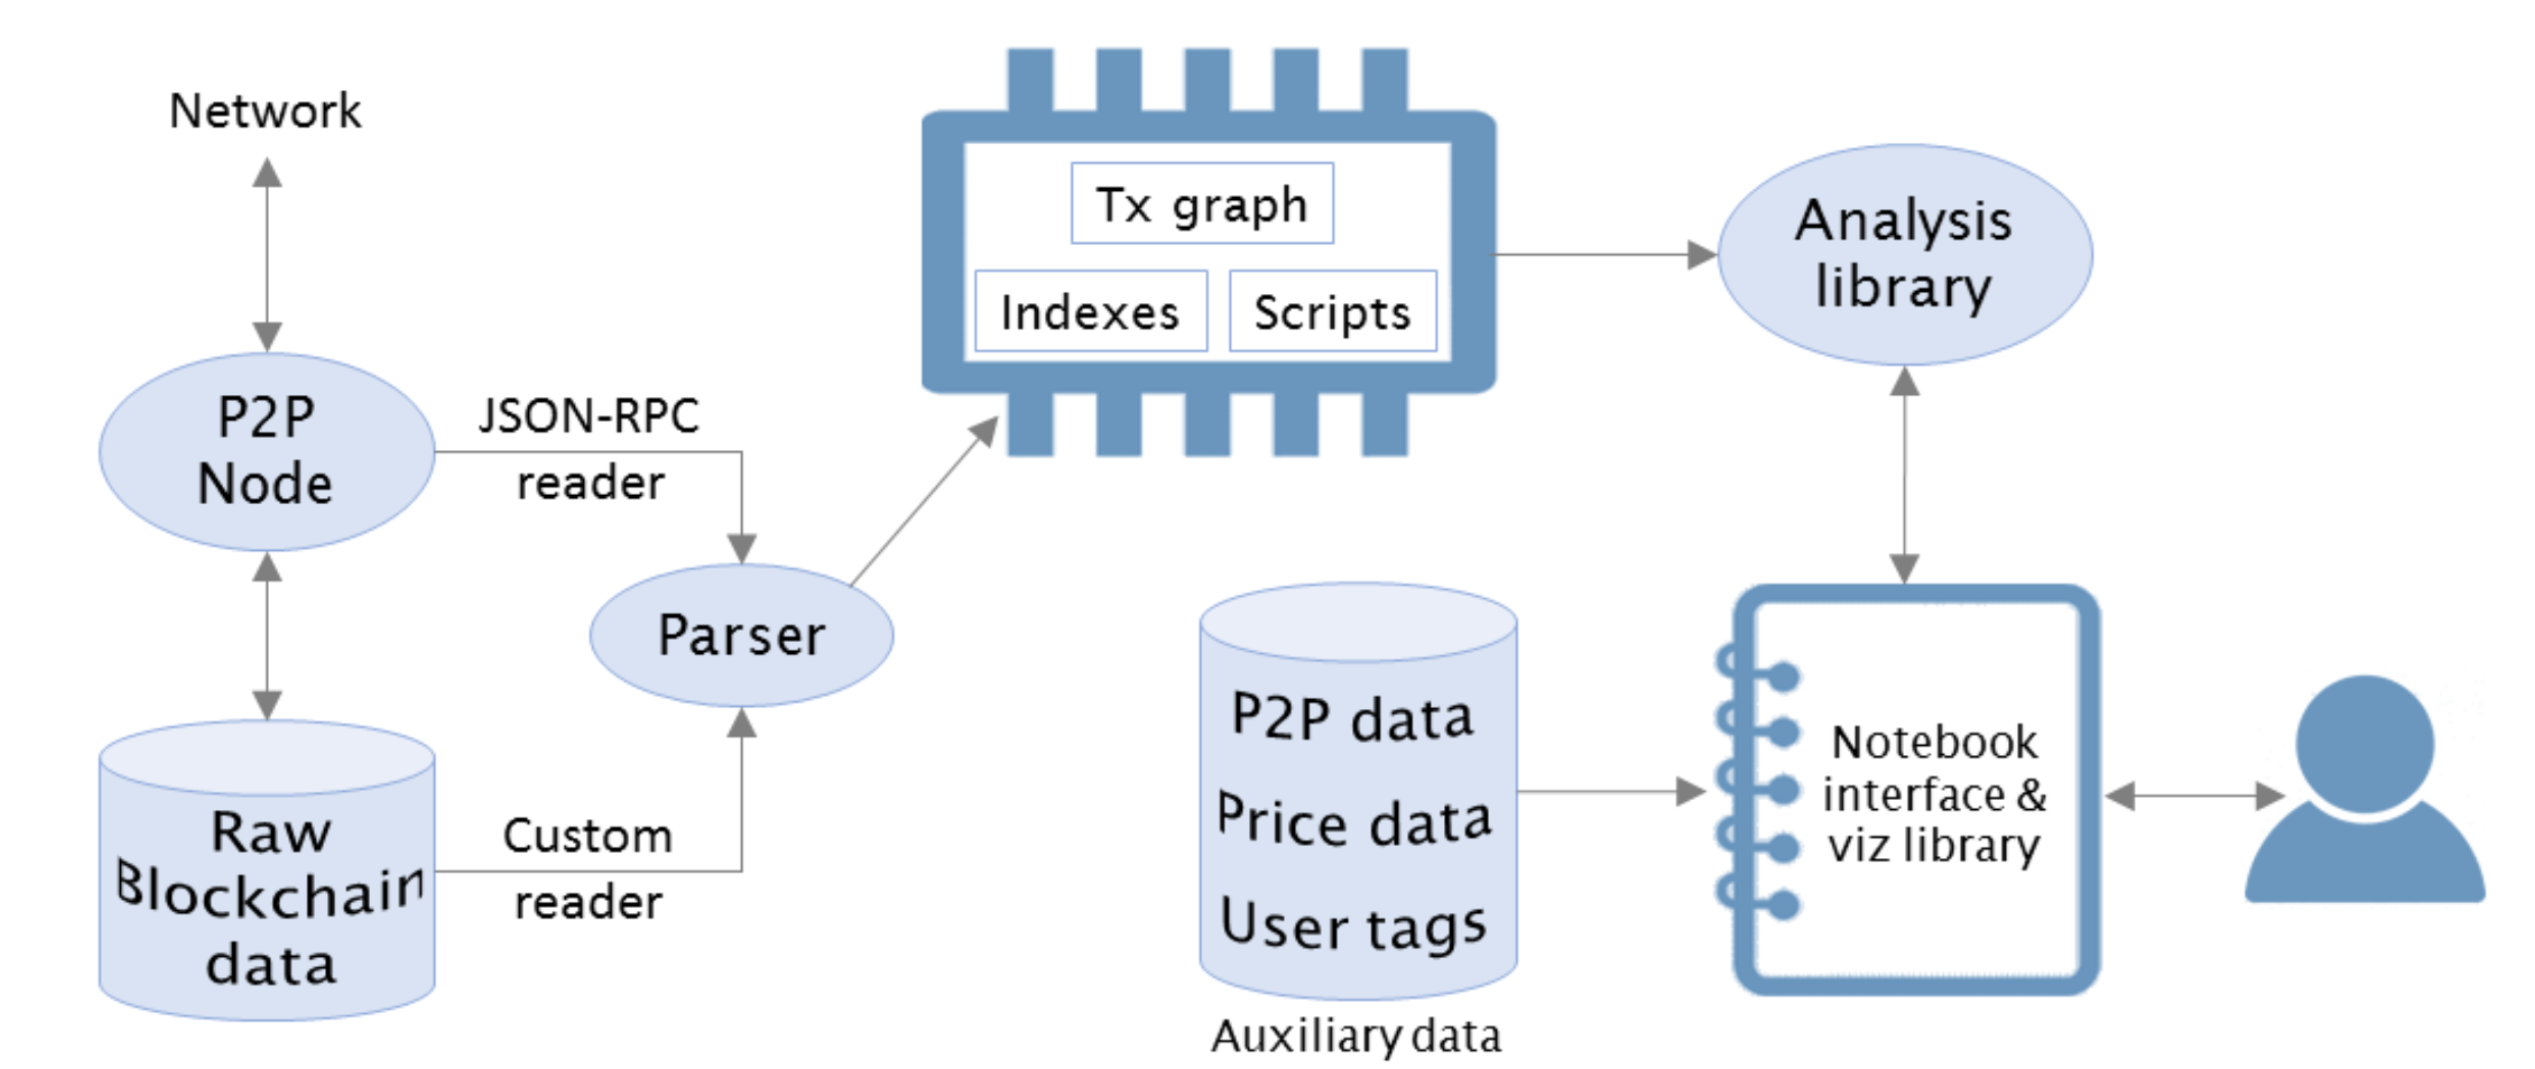
\includegraphics[width=.75\textwidth]{blocksci.png}
    \caption[Blocksci Architecture]{The main points of relevance in this figure are the parser and analysis library. As a brief summary, the P2P node refers to the BTC node running on the client, which is constantly getting updates as they are written to blockchain by miners. Thus, the raw blockchain data sitting on the client computer will be parsed and streamlined to produce the optimized iterable data structure, which gets updated as new information arrives from the P2P node. With this iterable struture, an analysis library can be layered atop, to perform work manyfold, one example of which is procuring heuristics and performing clustering \cite{blocksci}.}
    \label{fig:blocksci}
\end{figure}

In a similar vein, ``The on-disk format of blockchains is highly inefficient for our purposes. It is optimized for a different set of goals such as validating transactions and ensuring immutability...whereas we aim for a single representation of the data that can it in memory" \cite{blocksci}. In other words, the parser for Blocksci implemented many optimizations such that data structures were not as bloated as they are when stored on-disk, as validation was no longer of primary concern. Using such streamlining and properties of caching, iteration through the blockchain data was significantly optimized. Thus, the main takeway herein was that Blocksci made the procurement of additional heuristics atop the transactions graph an efficient process.

\subsection{Overview}
Having established the current state of the art in the deanonymization space, we now turn to presenting the necessary technical background. We begin with the layout of the investigation, from which all the pieces to be presented fall into place. Specifically, using the capabilities of Blocksci as elaborated upon above, we procured a set of eight heuristics, about which there are varying degrees of confidence. For sake of completeness, the heuristics are laid out here, as they are presented in \cite{heuristics}:

\begin{enumerate}
    \item Being shared inputs for a single transaction
    \item ``If input addresses appear as an output address, the client might have reused addresses for change.
    \item If all inputs are of one address type (e.g., P2PKH or P2SH), it is likely that the change output has the same type
    \item Most clients will generate a fresh address for the change. If an output is the first to send value to an address, it is potentially the change.
    \item Bitcoin Core sets the locktime to the current block height to prevent fee sniping. If all outpus have been spent, and there is only one output that has been spent in a transaction that matches this transaction’s locktime behavior, it is the change.
    \item If there exists an output that is smaller than any of the inputs it is likely the change. If a change output was larger than the smallest input, then the coin selection algorithm wouldn’t need to add the input in the first place.
    \item If tx is a peeling chain, returns the smaller output.
    \item Detects possible change outputs by checking for\dots values that are multiples of $10^{\text{digits}}$" \cite{heuristics}.
\end{enumerate}

With these heuristics, unlike previous investigations, we do not directly manipulate and collapse nodes of the original Bitcoin transaction graph. Instead, we procure a \textit{separate} graph, in which nodes correspond to wallets and edges represent the presence of a heuristic. If multiple heuristics are found to be true between two nodes, the edge connecting said nodes had the sum of the weights associated with the corresponding heuristics. In other words, denoting the weights for these heuristics as $w_1, w_2, ..., w_8$ where $w_i$ naturally takes some weight $\in[0,1]$ corresponding to heuristic $i$ and assuming these weights are normalized, such that $\sum_i w_i = 1$, if heuristics 2,3, and 4 come up as true between vertices $A,B$, the weight associated with edge $e_{AB}$ would be $w_2+w_3+w_4$.

Upon curating this heuristics graph, we sought to subsequently perform clustering. Unlike the previous investigations, however, clustering was implemented in the traditional graph theory sense rather than the union-find of previous papers. Such ``standard graph clustering" techniques entail algorithms like k-means, spectral, and DBSCAN, the specifics of which are elaborated upon subsequently in the background. This eventual clustering represents our final result, whose performance was measured by comparing against known addresses using multiple notions of clustering accuracy.

\subsection{Stochastic Block Model}
With that being said, this investigation began by modelling the heuristics graph in a simplified light, on which much of the initial experimentation and testing was performed. From here, many optimizations were tested and different clustering methods evaluated for use on the final dataset. The use case of studying a model rather than the full dataset is twofold. The first is that it allows rapid testing. That is to say, by being able to control exactly the size of the test graphs, many runs could be conducted for a given set of algorithms of interest. In line with that, the second benefit is having a defined metric by which performance could be measured. While there is a subset of known data points in the entire dataset, by having access to the full truth for a simulation, specific pain points could be evaluated. For example, if it turned out a particular algorithm worked well as measured by metric A but not so by metric B but metric A was of greater relevance to the final investigative result, we could easily make use of said algorithm in the final results run. In other words, such experiments made it such that the algorithms' strengths and weaknesses could be understood in great detail, since trials could be procured that targeted different circumstances.

In line with that, we begin our discussion with an introduction to the stochastic block model, commonly shortened to SBM. The SBM is a ``model for random graphs on $n$ nodes with two equal-sized clusters, with an between-class edge probability of $q$ and a within-class edge probability of $p$" \cite{sbm}. We, instead, focus on an expanded view of the SBM. That is to say, rather than solely being between two clusters, we define the SBM to have $n$ clusters such that for any clusters $C_i, C_j$, the probability a vertex in the first will be connected to a vertex in the second is $p$ if $i=j$ and $q$ if $i\neq j$, where $p > q$. In other words, this model produces a random graph comprised of many clusters, of respective sizes $n_1,n_2,...n_k$, with vertices more likely to be connected within a given cluster as compared to other clusters. This, therefore, roughly corresponds to our idealized form of the heuristics graph, namely where the heuristics would be more likely to be present between vertices that belong to the same cluster (i.e. same real-world entity). The main leak in this simplification arises from the fact that, in the case of the SBM, a single run will either have edges or not, with probability $p$ or $q$ depending on the vertices of interest whereas the heuristics graph \textit{always} has the weight just with a higher or lower value. However, in expectation, namely when averaged over a series of $n$ runs as $n\rightarrow\infty$, the adjacency matrix resembles that of the heuristics graph, specifically considering the case where the heuristic weights have been normalized:

\[
\sbox0{$\begin{matrix}p&p&p\\p&p&p\\p&p&p\end{matrix}$}
\sbox1{$\begin{matrix}q&q&q\\q&q&q\\q&q&q\end{matrix}$}
%
C=\left[
\begin{array}{c|c|c|c}
\usebox{0}&\makebox[\wd0]{\large $Q$}&\makebox[\wd0]{\large $\dots$}&\usebox{1}\\
\hline
\vphantom{\usebox{0}}\makebox[\wd0]{\large $Q$}&\makebox[\wd0]{\large $P$}&\makebox[\wd0]{\large $\dots$}&\makebox[\wd0]{\large $Q$}\\
\hline
\vphantom{\usebox{0}}\makebox[\wd0]{\large $\vdots$}&\makebox[\wd0]{\large $\dots$}&\makebox[\wd0]{\large $\ddots$}&\makebox[\wd0]{\large $\vdots$}\\
\hline
\vphantom{\usebox{0}}\makebox[\wd0]{\large $Q$}&\makebox[\wd0]{\large $\dots$}&\makebox[\wd0]{\large $\dots$}&\makebox[\wd0]{\large $P$}\\
\end{array}
\right]
\]

Where each of the block $P,Q$ entries are simply referring to $(p,q)\mathbbm{1}\mathbbm{1}^T$ respectively, as indicated in some of the matrix entries. The main limitation in the model arises in the fact that there is little to suggest different clusters will have similar weights in the heuristics graph. After all, it may be completely obvious that one set of vertices are in the same clustering, making their associated weight high, while another set of vertices have high uncertainty, making their weight lower, though the two should both be clustered. The natural extension to the SBM would simply involves having a different $p_i$ for each cluster $C_i$. Yet, this complicates the model to a degree that gaining the desired intuition of the clustering algorithms would not come with the same ease as it would could be otherwise. 

As a result, we sacrifice this piece of accuracy with the assumption that algorithm performance on this special case will scale appropriately to the general case. That is to say, we assume that, if algorithm A has better performance on the SBM than B, it should similarly perform better on the generalized case with varying $p_i$, though the two very likely will have degraded performance. The intuition reasoning behind said assumption is that the main detractor of performance will be when there are $p,q$ values that are comparable. Consider the edge case where $p=q$; clearly, this case can have no algorithm that performs clustering with any better accuracy than $50\%$. Thus, the bottleneck of the performance will be the lowest $p_i$ value and highest $q_{ij}$, where $q_{ij}$ denotes the natural extension of the notion of $q$ to arbitrarily many clusters, namely the probability that vertices from $C_i,C_j$ will be adjacent. However, we can consider a simulation in which $p,q$ are relatively near one another and evaluate the algorithms' performances on said case. Since this marks the worst/most difficult case, it follows that the best algorithm will similarly scale to be the best in the easier cases. This intuition, however, is confirmed through empirical testing in Section \ref{methodology}.

We finally present one noteworthy theorem of interest with relevance to SBMs, specifically the limitations with which they can be clustered. This makes more concrete the notion that if $p,q$ are ``sufficiently close," the graph clustering cannot be performed in any manner better than chance in the limit of large graphs (where $p=a/n,q=b/n$ for a graph with a total of $n$ vertices):

\begin{theorem}\label{thm:sbm}
If $a + b > 2$ and $(a-b)^2\le2(a+b)$ then, for any fixed vertices $u$ and $v$:

$$ \mathbb{P}_n(\sigma_u = + | G, \sigma_v = +) \rightarrow \frac{1}{2} \text{ a.a.s. \cite{sbm}} $$
\end{theorem}

Where $a.a.s.$ corresponds to asymptotically almost surely convergence. The specifics of this notion of convergence are not necessarily of relevance, though we put it here for sake of completeness. Namely, this corresponds to when ``An event $E$...holds with probability $1-o(1)$, thus the probability of success goes to $1$ in the limit $n\rightarrow\infty$" \cite{terry}. In other words, we cannot even determine whether two random vertices in the SBM are the same label or not better than random chance if $a,b$ are not sufficiently different. As demonstrate in Figure \ref{fig:region}, this corresponds to where $p,q$ are quite close to one another. Note that this region is symmetric about the line $x=y$, since the notions of $p,q$ can be flipped at any point and the complexity of clustering the model would remain the same. Since we are dealing with a generalized form of the SBM, we provide a straightforward extension of this theorem as follows:

\begin{figure}
    \centering
    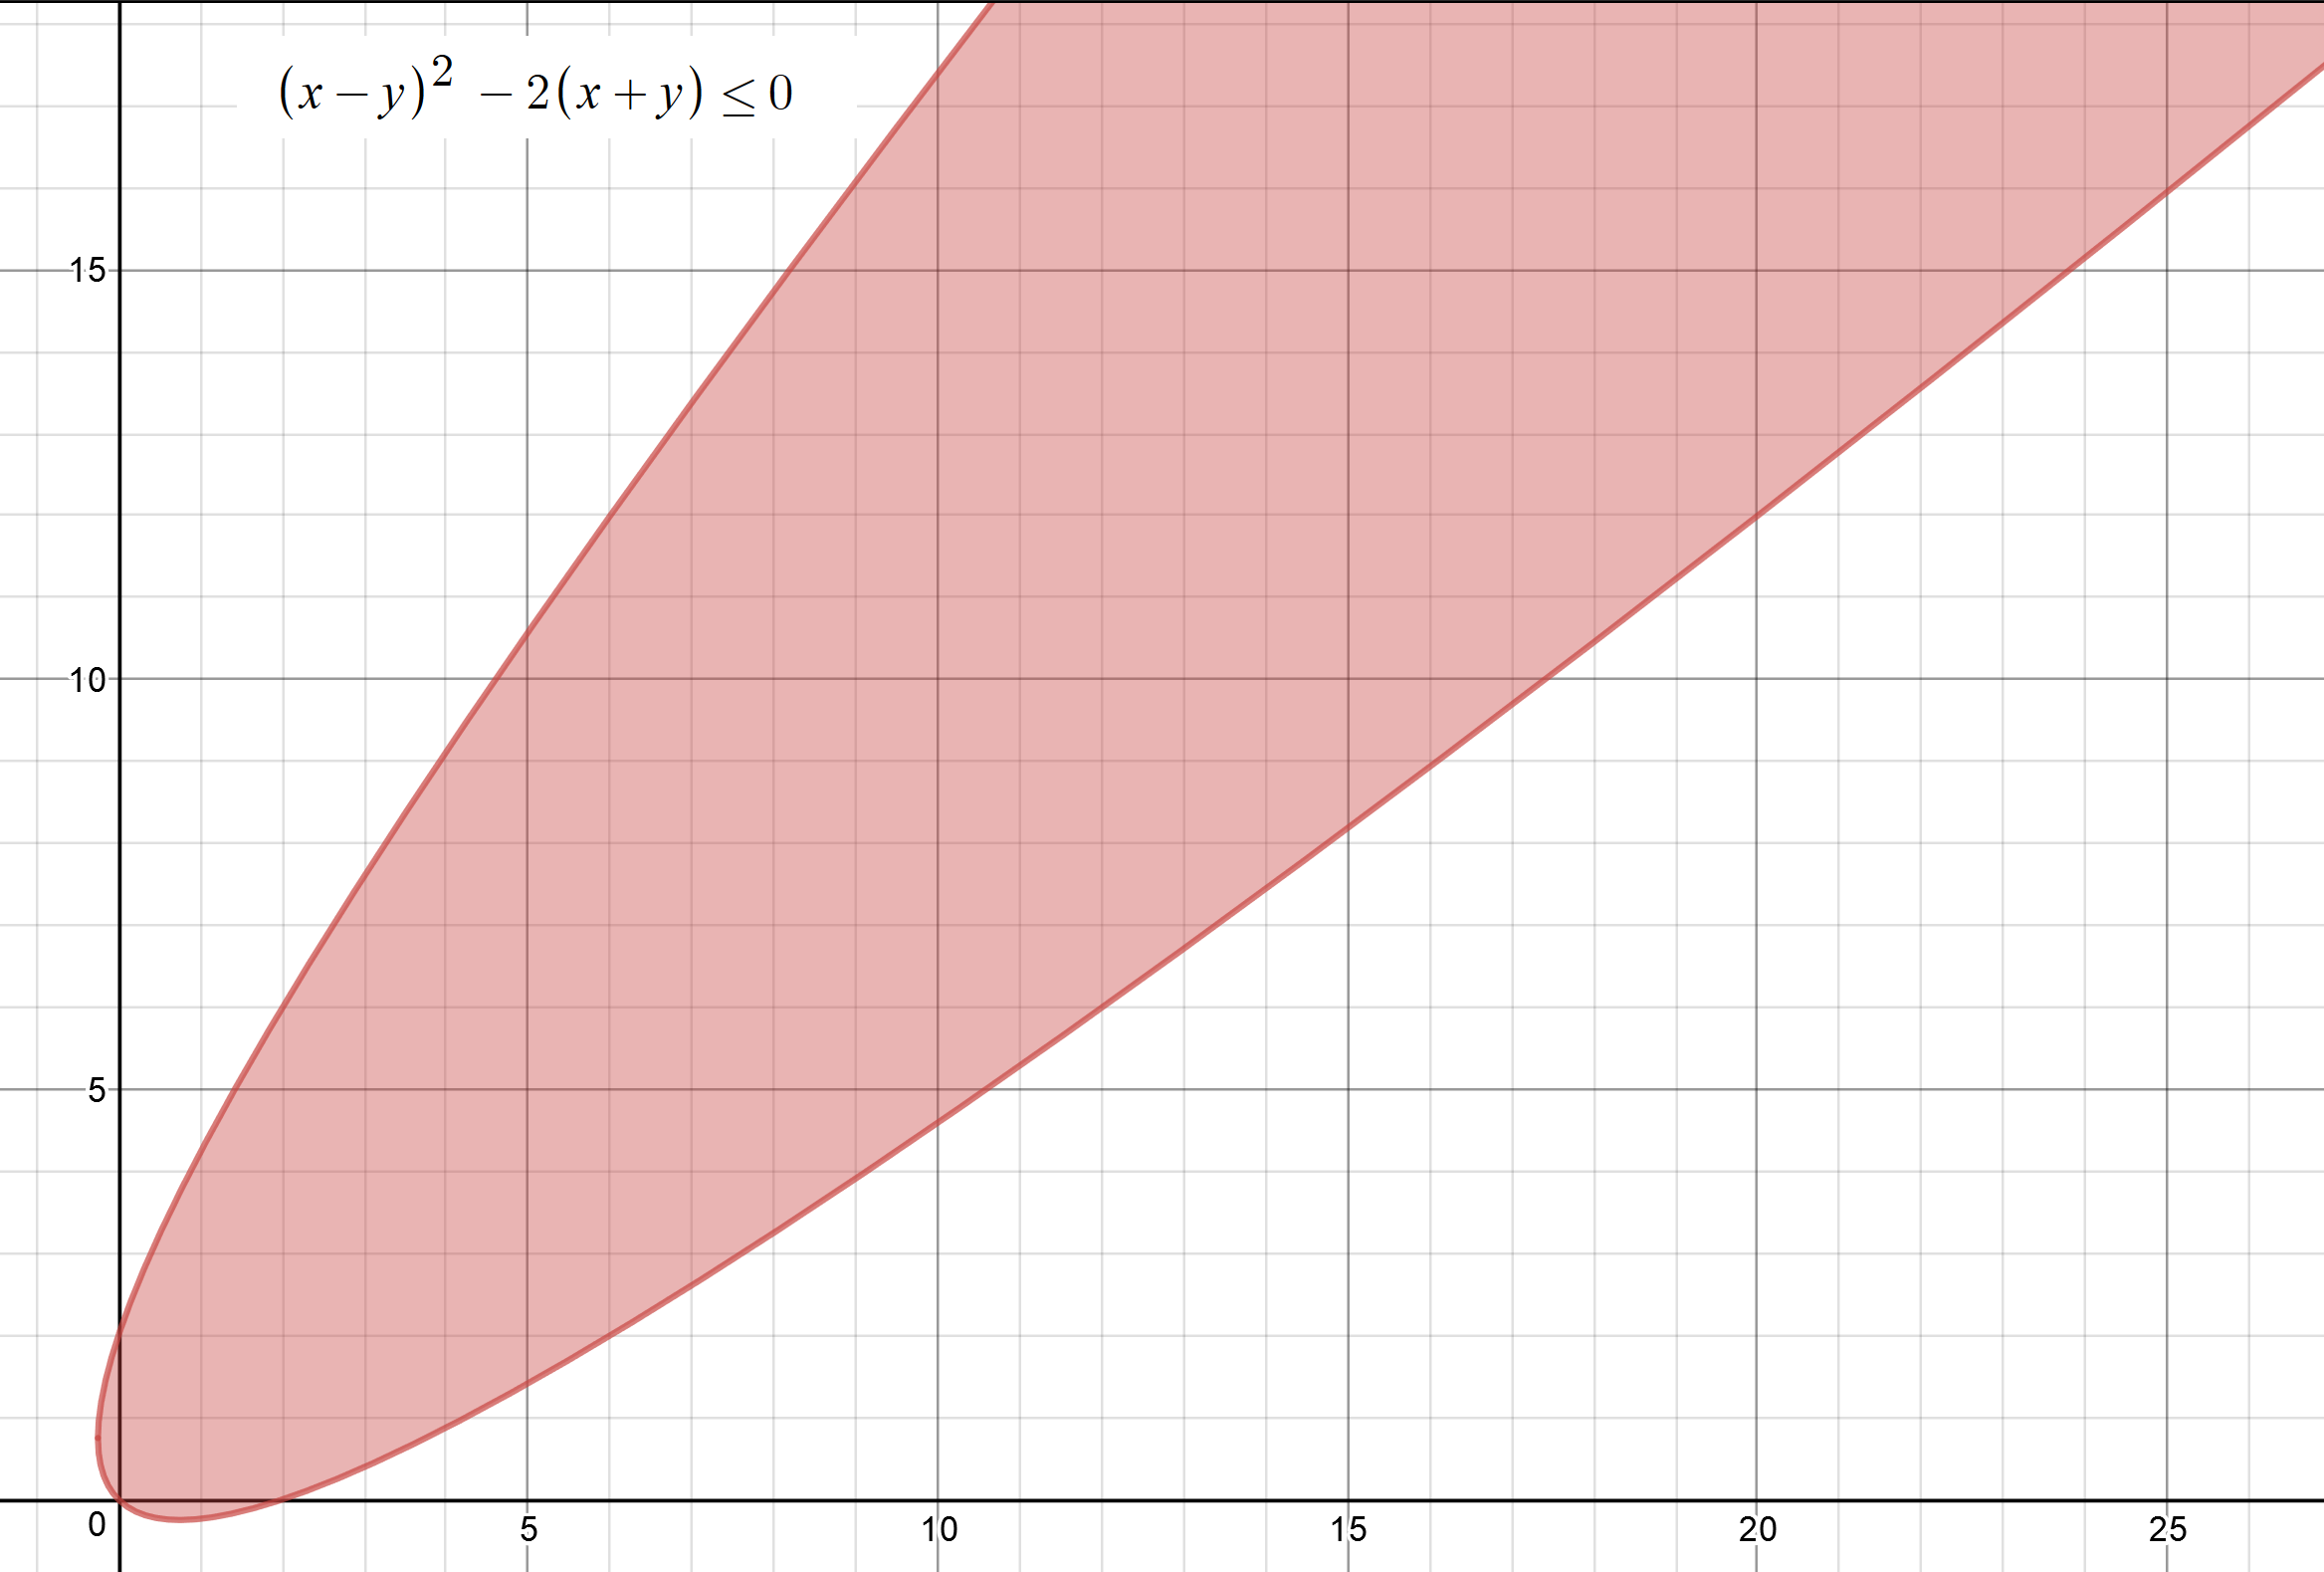
\includegraphics[width=.60\textwidth]{region.png}
    \caption[Region of No Deanonymization]{This marks the region in which no algorithm can perform clustering better than by chance. If the graph procured fell within this region, seeing as the $n$ considered for the heuristics graph was massive, it seems entirely infeasible that any algorithm would have reasonable performance.}
    \label{fig:region}
\end{figure}

\begin{corollary}
Assuming $G=\cup_{i}G_i=\bigcup_{i}(n_i,\frac{a_i}{n_i},\frac{b_i}{n_i})$, if for some choice $i$, $a_i + b_i > 2$ and $(a_i-b_i)^2\le2(a_i+b_i)$ then the problem of clustering is not solvable as $n\rightarrow\infty$.
\end{corollary}

\begin{proof}
The proof follows as a trivial consequence of the previously relayed theorem. A clustering problem is considered solvable when ``one can $a.a.s.$ find a [cluster] which is positively correlated with the" true cluster \cite{sbm}. As any clustering algorithm must inherently cluster all subgraphs of $G$, simply consider its clustering on $G_i$, there is no positive correlation in the limit of $n\rightarrow\infty$ by Theorem \ref{thm:sbm}. The overall correlation, therefore, must similarly be non-positive, meaning this overall clustering task is unsolvable.
\end{proof}

Hence the main takeaway from this section is that the SBM serves as a very pertinent simplification of the heuristics graph on which many of the properties of the clustering algorithms could be understood through relevant experiments.

\subsection{Clustering Algorithms}
Moving on from the SBM, we look to discussing the second topic at hand, specifically graph clustering. We present the relevant algorithms, followed by specific extensions that we employed due to the massive scale of the data considered herein. This discussion of clustering is summarized in a table presented following all the sections, namely Table \ref{tab:algs}. We further assume that when referring to graph clustering, we wish to separate the set $V$ corresponding to $G$ into sets $\{C_1, C_2, ..., C_n\}$, such that $\bigcap_{i} C_{i} = \emptyset$, where the objective is to minimize the ``distance" between vertices in a single $C_i$ and maximize that between any $C_i,C_j$ for $i\neq j$, where ``distance" often has a natural interpretation as related to edge weights in the graph. 

\subsubsection{k-means}
k-means is the canonical example of a clustering algorithm. Given its age and the continual improvements in efficiency, k-means can be run efficiently on massive datasets. Specifically, k-means works ``given an integer $k$ and a set of $n$ data points in $\mathbb{R}^d$ , the goal is to choose $k$ centers so as to minimize $\phi$, the total squared distance between each point and its closest center" \cite{k-means}. The clustering of points, therefore, is simply according to which mean they are located nearest to. The determination of such $k$ clusters, however, is an NP-hard problem, for which a heuristic has been developed and repeatedly confirmed in practice. This employed heuristic works as follows: it ``begins with k arbitrary `centers,' typically chosen uniformly at random from the data points. Each point is then assigned to the nearest center, and each center is recomputed as the center of mass of all points assigned to it. These last two steps are repeated until the process stabilizes" \cite{k-means}. 

Thus, as with many of the other algorithms considered below in this paper, k-means requires prior knowledge of the number of clusters. We take an aside to address this point. While it may seem wholly arbitrary that the number of clusters be known ahead of time, as there is little way to ascertain ahead of time how many \textit{unique} users of Bitcoin there are on the network, this serves as a means by which the granularity of results can be controlled. That is to say, given two identical networks, we could potentially extract more fine clusterings with higher levels of $k$. For example, in the edge case of $k=2$, the clustering would likely resemble something along the lines of ``Coinbase accounts" and ``non-Coinbase accounts," namely a separation of a supercluster from the remainder of the graph. We can, therefore, imagine that as $k\rightarrow\infty$, clusters associated with individual people or small organizations would form out of the massive agglomerated ``Non-Coinbase" cluster. In the limit, however, we would simply end up with singleton clusters, which would serve little purpose for identifying real-world entities. The selection of $k$, therefore, is a balancing act between getting fine grain separation of individual entities and uninformative results.

Thus, the main use case of k-means herein will be as a baseline for getting results. That is to say, we expect \textit{all} other algorithms employed to have superior performance than k-means, though they may suffer greatly in time complexity.

\subsubsection{Spectral}\label{spectral-bg}
Spectral clustering, as implied by its name, deals with clustering on the basis of eigenvalues and eigenvectors. Which eigenvectors to be used for such clustering is not immediately obvious. However, it turns out to be those of a matrix that has fundamental importance to its corresponding graph: the Laplacian. While the Laplacian has differing definitions by context, in the realm of graph theory, it simply refers to:

$$ L = D-W $$

Where hereafter we denote the Laplacian matrix as $L$; the degree matrix as $D$, which contains the degree of vertex $i$ in position $D_{ii}$ and 0s elsewhere; and the weight matrix as $W$, which contains the weight of edge $e_{ij}$ in position $D_{ij}$. Since $D,W$ are both symmetric matrices in the case of an undirected graph, $L$ too is symmetric. Having presented the definition, we follow up with some relevant theorems regarding this Laplacian matrix \cite{spectral}:

\begin{theorem}
\begin{itemize}
    \item[] \mbox{}
    \item The smallest eigenvalue of $L$ is $0$. The corresponding eigenvector is the constant one vector $\mathbbm{1}$.
    \item $L$ has $n$ non-negative, real-valued eigenvalues $0=\lambda_1\le\lambda_1\le\dots\le\lambda_n$.
\end{itemize}
\end{theorem}

From this theorem spawn several other results which have direct consequences in the use of eigenvectors for the purposes of graph clustering. The first theorem is as follows:

\begin{theorem}
Let $G$ be an undirected graph with non-negative weights. Then the multiplicity $k$ of the eigenvalue 0 of $L$ equals the number of connected components $A_1,\dots,A_k$ in the graph. The eigenspace of eigenvalue $0$ is spanned by the indicator vectors $\mathbbm{1}_{A_1},\dots,\mathbbm{1}_{A_k}$ of those components.
\end{theorem}

While we refer to \cite{spectral} for the whole proof of this result, we present a sketch of the primary portion of this proof from which an intuitive understanding arises. Specifically, consider the idealized case of a graph $G$ containing clusters such that vertices within the clusters are fully connected and those in different clusters are not adjacent. The corresponding graph Laplacian for such a $G$ would be:

\[
\begin{bmatrix}
    L_{1} &  & &  \\
    & L_{2} & &  \\
    & & \ddots &  \\
    & & & L_{n}
\end{bmatrix}
\]

Where each $L_i$ is the Laplacian of the subgraph that only contains cluster $i$. From here, we notice that the eigenvectors of $L$ are simply those that correspond to those of each of the $L_i$ with 0s filling up the entries that do not correspond to the $L_i$ matrix entries. By the preceding thereom, we know that each of these sub-Laplacians has an eigenvector of $\mathbbm{1}$ corresponding to the eigenvalue 0, meaning that the multiplicity of the eigenvalue 0 relates to how many block entries there are in this Laplacian matrix, which precisely corresponds to the number of clusters there are. 

We now wish to understand how to go about using such eigenvectors to accomplish clusterings. Specifically, to do so, consider once again the idealized case. In creating a matrix of these $k$ eigenvectors as columns, we are left with a matrix of the form (where we are depicting the matrix as if the clusters are all of size 2):

$$ M = [\mathbbm{1}_{A_1}^T,\mathbbm{1}_{A_2}^T,\dots,\mathbbm{1}_{A_k}^T] = 
\overbrace{\begin{bmatrix}
    1 & 0 & \dots & 0 \\
    1 & 0 & \dots & 0 \\
    0 & 1 & \dots & 0 \\
    0 & 1 & \dots & 0 \\
    \vdots & \vdots & \ddots & \vdots \\
    0 & 0 & \dots & 1
\end{bmatrix}}^{k}
$$

From here, we simply notice that there are precisely as many rows as there were originally vertices in the graph, since each column corresponds to an eigenvector. Noticing that, it becomes clear that if we associate each vertex with its corresponding row, these vertices can now be trivially clustered using k-means with perfect accuracy. Thus, the main takeaway from this example is understanding that the eigenvectors corresponding to eigenvalues of lowest magnitude essentially help transform the vertices into a new space that much more closely correspond to their associated cluster, from which the k-means algorithm can trivially be employed to complete clustering. The eigenvectors with lowest eigenvalues are employed as they are the ones closest to the idealized $\mathbbm{1}_{A_i}$ vectors. 

An interesting addition supplied by spepctral clustering arises in its eigenvalue roughly serving to indicate how separable certain subsets of the vertices are. In turn, eigenvalues of low and high magnitude are easily separated. As a result, we can estimate the number of clear clusters, namely by determining how many eigenvalues are near 0 prior to there being a jump in magnitude, as portrayed in Figure \ref{fig:spectral_example}.

\begin{figure}
    \centering
    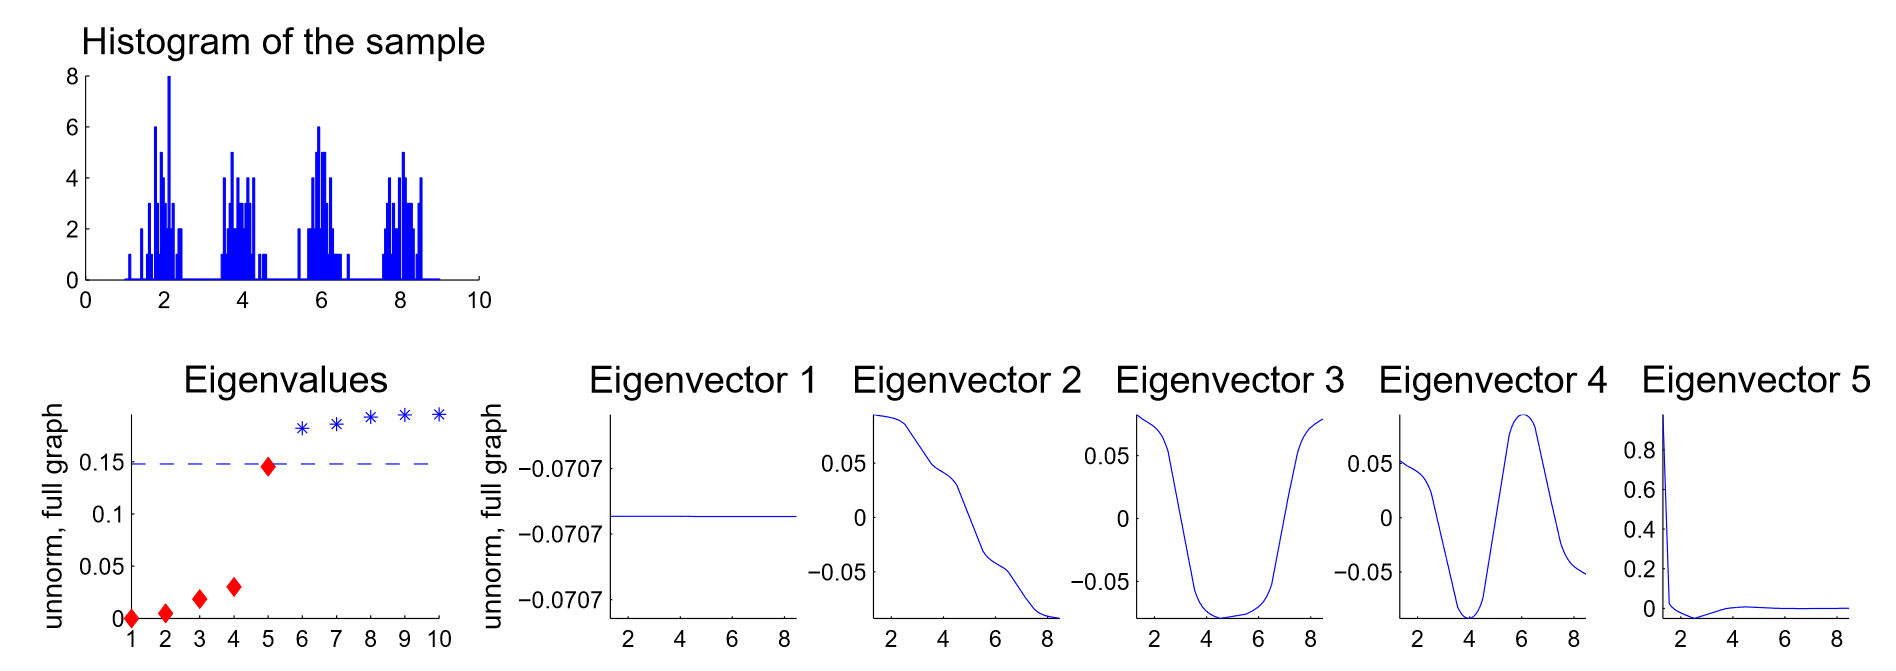
\includegraphics[width=.95\textwidth]{spectral_example.png}
    \caption[Spectral Eigenvector]{The top left is a histogram of the data spread, and the remainder of the picture corresponds to the eigenvalues and eigenvectors of the Laplacian, as discussed in the exposition. From this, it is clear that a well-separated dataset has a marked jump between eigenvalues that correspond to the the clusters and those that do not \cite{spectral}.}
    \label{fig:spectral_example}
\end{figure}

This procedure is summarized in the presentation of Algorithm \ref{alg:spectral-kmeans}. Note that their conception of spectral clustering involves beginning with a similarity matrix, namely a symmetric matrix where entry $S_{ij}$ corresponds to some notion of ``similarity" between vertices $i,j$. It is from this matrix that a similarity graph is \textit{constructed} and its Laplacian determined. There exist many ways by which such a similarity graph can be constructed. As enumerated in \cite{spectral}, three such ways are as follow:

\begin{itemize}
    \item \textbf{$\epsilon$-neighborhood graph}: Connect vertices together if the similarity metric defined between the two of them exceeds some threshold parameter value of $\epsilon$. That is to say, the adjacency matrix will have edges according to $I_{e_{ij}>\epsilon}$.
    \item \textbf{$k$-nearest neighbors}: Connect a given vertex to its $k$ nearest neighbors in sense defined by the similarity metric, i.e. create an edge for the vertices corresponding to the $k$ highest similarity measures. While this is normally asymmetric, simply avoid this problem by creating an undirected edge between the two vertices. That is to say, an edge between $v_i,v_j$ will be present if \textit{either} $v_j$ is one of the $k$-nearest neighbors for $v_i$ or vice versa (or both).
    \item \textbf{Fully-connected graph}: Connect all edges, weighting the edges with some similiarity function, i.e. a Gaussian $G(v_i,v_j) = \text{exp}\left(-\frac{|| v_i - v_j ||^2}{2\sigma^2}\right)$
\end{itemize}

For our particular case, we elected to use the third method of catering a similarity graph, although future elaborations on this work may expand this assumption and attempt other methods to determine their relative success. 

\begin{algorithm}
    
\caption{Constructs Laplacian from the similarity matrix \cite{spectral}}\label{alg:laplacian}
\begin{algorithmic}[1]
\Procedure{ConstructLaplacian(S,k)}{} \\
\textbf{Input:} Similarity matrix $S\in\mathbb{R}^{n\times n}$ \\
\textbf{Input:} Cluster count $k$

\State $G \gets \text{Similarity graph for } S$
\State $W\in\mathbb{R}^{n\times n} \gets \text{Weighted adjacency matrix for } G$
\State $L \gets D - W$ \\

\textbf{Output:} Laplacian matrix $L$
\EndProcedure
\end{algorithmic}
\end{algorithm}

\begin{algorithm}
\caption{k-means based spectral clustering \cite{spectral}}\label{alg:spectral-kmeans}
\begin{algorithmic}[1]
\Procedure{SpectralClustering-Kmeans(S,k)}{} \\
\textbf{Input:} Similarity matrix $S\in\mathbb{R}^{n\times n}$ \\
\textbf{Input:} Cluster count $k$

\State $L \gets ConstructLaplacian(S,k)$
\State $v_1,v_2,...,v_k \gets \text{first } k \text{ (sorted by } \lambda_i \text{) eigenvectors of } L$
\State $V\in\mathbb{R}^{n\times k} \gets [v_1^T, v_2^T,\dots,v_k^T]$
\State $(y_i)_{i=[1:k]} \gets V^T_{i,:} \text{ (i.e. row } i \text{ of } V\text{)}$
\State $(C_i)_{i=[1:k]} \gets kmeans((y_i)_{i=[1:k]})$ \\
\textbf{Output:} $(C_i)_{i=[1:k]}$
\EndProcedure
\end{algorithmic}
\end{algorithm}

In addition to this method of implementing spectral clustering, however, there is another which relies on a different principle, albeit still related to the spectrum of the Laplacian matrix. In this alternate approach, the ``eigenvector $u_2$ corresponding to $\lambda_2$ (the second-smallest eigenvalue) is computed, and the vertices of the graph are partitioned according to the values of their corresponding entries in $u_2$" \cite{bisection}. In other words, the second eigenvector is computed and used to partition the graph into two (or three) sections, specifically corresponding to the signs of the components of the eigenvector. This process can be subsequently repeated a number of times to achieve the desired number of $k$ clusters. Subsequent iterations bisect the cluster with the lowest second eigenvalue, since this effectively corresponds to how well separable the cluster is, meaning after $k$ iterations $k+1$ clusters would exist.

Returning to the previous example at hand, namely the idealized case, intuition for this algorithm becomes clear. Specifically, we have that the eigenvector of the first eigenvalue (which \textit{always} corresponds to an eigenvalue of 0) will simply be $\mathbbm{1}$, meaning there is no information to be gleaned from its entries. Instead using the second eigenvector, we have something of the form $[\textbf{0}_{A_1},\dots\textbf{0}_{A_{k-1}},\mathbbm{1}_{A_k},\dots\textbf{0}_{A_n}]$. In this case, we see that partitioning by sign would effectively separate a cluster ($A_k$ in this particular instance) from the remainder of the graph. Presumably, in the following iteration, the second eigenvalue corresponding to the subgraph of $G\backslash A_k$ will be less than that of $A_k$, meaning it will be partitioned in the following iteration. Once again, the second lowest eigenvalue is chosen as it roughly demonstrates that the corresponding cluster is the closest to the idealized separable case of all those present in the clustering. We refer to this version of spectral clustering as ``hierarchical," as it involves repeated bisection and employs a top-down separation method as contrasted with the k-means spectral implementation, which clusters all vertices at once. It seems natural, therefore, to expect hierarchical to be more accurate but significantly slower, due to its more careful handling of separation, than its k-means counterpart, a trend we investigated more fully empirically. This procedure is fully summarized in Algorithm \ref{alg:spectral-hierarchical}. 

\begin{algorithm}
\caption{Hierarchical based spectral clustering \cite{spectral}}\label{alg:spectral-hierarchical}
\begin{algorithmic}[1]
\Procedure{SpectralClustering-Hierarchical(S,k)}{} \\
\textbf{Input:} Similarity matrix $S\in\mathbb{R}^{n\times n}$ \\
\textbf{Input:} Cluster count $k$

\State $C \gets [G]$
\For {$i=1:k-1$}
    \State $\lambda_{min} \gets None$, $v_{min} \gets None$, $j_{min} \gets None$
    
    \For {$j=1:len(C)$}
        \State $W\in\mathbb{R}^{n\times n} \gets \text{Adjacency matrix for } C[j]$
        \State $L_j \gets D_j - W_j$
        \State $\lambda_2,v_2\gets\text{2nd eigenvalue, eigenvector of } L_j$
        \If {$\lambda_2 < \lambda_{min}$}
            \State $\lambda_{min} = \lambda_2$
            \State $v_{min} = v_2$
            \State $j_{min} = j$
        \EndIf
    \EndFor
    
    \State $C_{new} = [Set(),Set()]$
        \For {$k=1:len(v_{min})$}
            \If {$v_{min}[k] > 0$}
                $C_{new}[0].add(v_{min}[k])$
            \Else 
                $C_{new}[1].add(v_{min}[k])$
            \EndIf
        \EndFor
        
    \State $C[j_{min}] \gets C_{new}$
\EndFor \\

\textbf{Output:} $C$
\EndProcedure
\end{algorithmic}
\end{algorithm}

Thus, having discussed spectral clustering, we briefly discuss its role in this investigation. Spectral clustering represents one of the major departures from previous studies that we wished to bring forward to this investigation, since it markedly involves attempting to perform clustering in a higher dimensional space, to capturing non-planar clusters. This contrasts previous studies, whose clustering, by virtue of directly working with the transaction graphs, cannot obtain any results that are non-planar. Hence, we wished to observe whether any clusters are more easily discernable under the mapping produced in spectral clustering as compared to their planar counterparts.

\subsubsection{DBSCAN}
DBSCAN is markedly different from the previous two algorithms in that it expressly seeks to be an algorithm that does not need a number of clusters to be supplied. Much in the way spectral clustering can be used to estimate the number of clusters using a ``separation gap," DBSCAN similarly relies on two user-supplied parameters to effectively serve as the thresholds to be considered as part of the same cluster, though the manner in which these parameters serve as a threshold is slightly more involved. Prior to diving more in depth about its inner workings, it is noteworthy that DBSCAN additionally does not necessarily cluster all vertices. That is to say, many of the vertices may end in a state of being in an ``undefined" category with respect to how it clusters. This is quite natural, in that there are often circumstances where vertices are simply shoehorned into a particular premade cluster simply because it is the best of the available options when in reality it is clear said vertex does not fit well in \textit{any} of these clusters.

Returning to the algorithm at hand, the user-supplied parameters are typically denoted as $\epsilon$ and $minPts$. From these, a set of ``core points" $\{p_i\}$ are defined, where a core point is any point $p\in G$ such that there are $\ge minPts$ other points $q$ such that the distance $d_{pq} < \epsilon$. That is to say, a core point essentially captures the intuitive notion of certain vertices being ``central" in the graph, i.e. being well-connected to a significant number of other vertices in the graph. From there, we define one vertex $v_B$ as being \textit{directly} reachable from another $v_A$ if the other vertex is a distance $d_{AB} < \epsilon$. We now define an arbitrary vertex $v_B$ as being reachable from another $v_A$ if there is a path of pairwise directly reachable core points that terminate in $v_B$. This is more clearly illustrated in Figure \ref{fig:dbscan}.

To finally construct the clusters, we simply go through the set of core points and find all other vertices that are reachable from these seeds. If a vertex is not reachable from any core points, it is simply remains unclustered in the final result \cite{dbscan}.

\begin{figure}
    \centering
    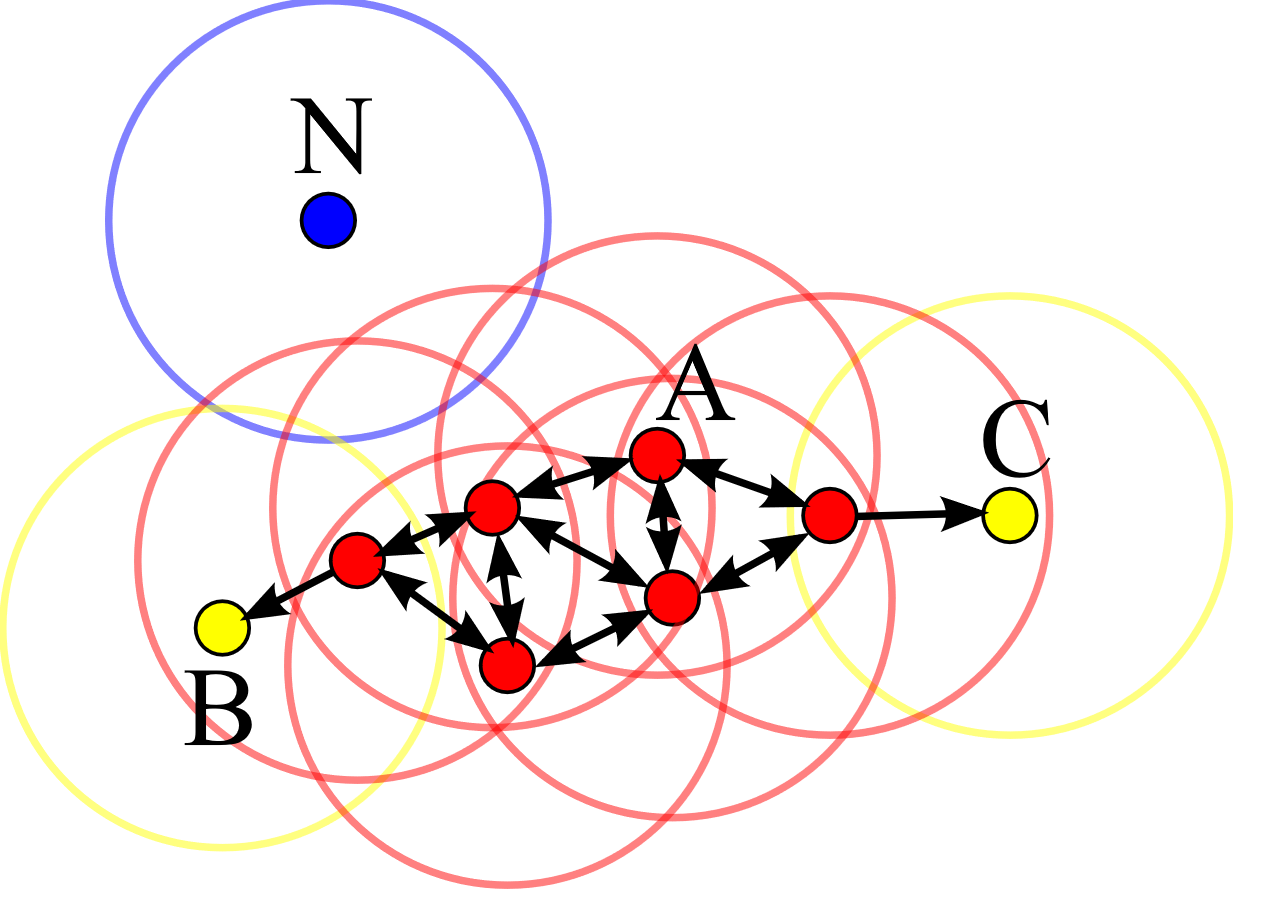
\includegraphics[width=.50\textwidth]{dbscan.png}
    \caption[DBSCAN Clustering]{Here the $minPts=4$. Red points correspond to the core points, yellow those that are reachable from core points, and blue that not reachable from any. Thus, in this case, all the vertices would be clustered together with the exception of the blue vertex \cite{wiki-dbscan}.}
    \label{fig:dbscan}
\end{figure}

The main advantage of DBSCAN is that it is extremely well suited for large-scale clustering. DBSCAN additionally is capable of capturing non-flat cluster geometry, similar to spectral clustering, due to its ability to capture long-link separated clusters. Thus, it provides a means of clustering that effectively takes the superior speed of k-means and clustering flexibility of spectral into a single algorithm. Unfortunately, DBSCAN is extremely sensitive to parameter selection, and the choices are oftentimes non-obvious, as they hold little semantic meaning outside of the context of the algorithm itself.

To summarize, we present these strengths and necessary parameters are presented in Table \ref{tab:algs}. Note that this summary table was procured by \texttt{scikit-learn}, meaning there could be variations in implementation details of these algorithms that see parameter use differently.

\begin{table}[]
\centering
\caption[Clustering Algorithm Summary]{Summary of clustering algorithms \cite{scikit}.}
\label{tab:algs}
\begin{tabular}{llll}
\textbf{Method name} & \textbf{Parameters} & \textbf{Scalability}                                                                                     & \textbf{Use Case}                                                                                                   \\ \hline
K-Means              & number of clusters  & \begin{tabular}[c]{@{}l@{}}Very large n\_samples, medium \\ n\_clusters with Minibatch code\end{tabular} & \begin{tabular}[c]{@{}l@{}}General purpose, even cluster size, \\ flat geometry, not too many clusters\end{tabular} \\ \hline
Spectral clustering  & number of clusters  & \begin{tabular}[c]{@{}l@{}}Medium n\_samples, \\ small n\_clusters\end{tabular}                          & \begin{tabular}[c]{@{}l@{}}Few clusters, even cluster size, \\ non-flat geometry\end{tabular}                       \\ \hline
DBSCAN               & neighborhood size   & \begin{tabular}[c]{@{}l@{}}Very large n\_samples, \\ medium n\_clusters\end{tabular}                     & \begin{tabular}[c]{@{}l@{}}Non-flat geometry, uneven \\ cluster sizes\end{tabular} \\ \hline
\end{tabular}
\end{table}

\subsection{Clustering Evaluation}\label{evaluation}
Having discussed these clustering methods, it seems natural that there be a metric by which they can be compared. This seemingly trivial property, however, is not completely obvious in its definition as it may seem upon first glance. Specifically, we assume for the sake of this discussion that there is some known ground truth clustering of the vertices. Unlike the DBSCAN assumption, we further assume that \textit{all} vertices are associated with one (and exactly one) cluster of the ground truth. 

Having said that, there emerge four natural metrics of evaluating clustering, per \cite{evaluation}. The notation employed by this resource, and that which we extend for the remainder of this section, is `` $\Omega = \{ \omega_1, \omega_2, \ldots, \omega_K \}$is the set of clusters and $\mathbb{C} = \{ c_1,c_2,\ldots,c_J \}$  is the set of classes" \cite{evaluation}. In other words, $\Omega$ corresponds to the guessed clusters while $C$ is the set of ground truth clusters, which are referred to as ``classes." 

The first metric is referred to as \textit{purity} and is defined as:

$$ \text{purity}( \Omega,\mathbb{C} ) = \frac{1}{N} \sum_k \max_j \vert\omega_k \cap c_j\vert $$

Roughly, the intuition behind purity is that a clustering with high purity has clusters such that the elements that are clustered together in truth originate from the same class. Thus, a perfect clustering would have a purity of 1.0. However, it also follows that as $k\rightarrow\infty$, the purity will tend towards 1.0 and will be exactly so once $k=n$. In other words, once there are sufficiently many clusters that each vertex gets associated to its own cluster, the purity there and for any higher values of $k$ will be 1.0. Thus, this metric, while useful in ascertaining the overlap with the true classification, suffers from generally rewarding high granularity. 

Another metric is the ``normalized mutual information or NMI:

$$ \text{NMI}(\Omega , \mathbb{C}) = \frac{ I(\Omega ; \mathbb{C}) } { [H(\Omega)+ H(\mathbb{C} )]/2 } $$

[where] $I$ is mutual information

\begin{align}
I( \Omega ; \mathbb{C} ) &= \sum_k \sum_j P(\omega_k \cap c_j) \log \frac{P(\omega_k \cap c_j)}{P(\omega_k)P(c_j)} \\
&= \sum_k \sum_j \frac{\vert\omega_k \cap c_j\vert}{N} \log \frac{N\vert\omega_k \cap c_j\vert}{\vert\omega_k\vert\vert c_j\vert}
\end{align}

where $P(\omega_k)$, $P(c_j)$, and $P(\omega_k \cap c_j)$ are the probabilities of a document being in cluster $\omega_k$, class $c_j$, and in the intersection of $\omega_k$ and $c_j$, respectively...$H$ is entropy...:

\begin{align}
H(\Omega) &= -\sum_k P(\omega_k) \log P(\omega_k) \\
&= -\sum_k \frac{\vert\omega_k\vert}{N} \log \frac{\vert\omega_k\vert}{N}
\end{align}

where...the second equation is based on maximum likelihood estimates of the probabilities" \cite{evaluation}. Having presented this metric, it serves well to parse the definition. The intuition behind this metric becomes more evident in understanding the notions of mutual information and entropy separately. In fact, the latter is simply a special case of the former, where $H(\Omega) = I(\Omega,\Omega)$. Returning to mutual information, this measures the gain in information from being presented a new piece of information. Intuitively, it is the reduction in uncertainty of the state of some random variable $B$ by learning that for some r.v. $A$. In this particular case, it is measuring the extent to which knowing our guessed clusters helps in knowing the class. Clearly, in the case of a perfect reconstruction of the true clustering, knowing our guess will give complete knowledge of the associated class, whereas an ill-formed guess will give no bearing as to what the true class is.

It, once again, follows that the mutual information increases to its max value as $k\rightarrow\infty$, namely once there are sufficiently many clusters to assign one per vertex. Taking an aside, as previously discussed, if we are able to recreate the ground truth clusters perfectly, the maximum value of MI is achieved. However, by looking at the definition, it becomes clear that if these clusters are further subdivided, the resulting MI remains the same. That is to say, if we have one additional cluster than the number present in the ground truth but the clusters $C_1,\dots,C_{n-1}$ correspond exactly to those in the truth and $C_n,C_{n+1}$ split the underlying $n$th true cluster, the MI will still be maximized. In particular, this means in the case of each vertex being assigned to its own cluster, as this is a refined clustering of the ground truth, the max MI will \textit{also} be attained in this case. Thus, to combat this issue, we normalize by the entropy, which ``tends to increase with the number of clusters" \cite{evaluation}. Thus, by combining these two into a single NMI metric, we are able to effectively measure that the correct number of clusters were extracted in addition to the contents of the clusters being correctly formed.

The final two metrics are directly related to one another, with thie third simply being a special case of the fourth. This metric, known as the Rand index, is, in fact, the simplest to present and interpret. We simply consider all $n(n-1)/2$ pairs of vertices and calculate:

$$ RI = \frac{TP + TN}{TP + TN + FP + FN} $$

Where TN, TP, FP, and FN are respectively the true negative, true positive, false positive, and false negative classifications that were made. Thus, if a pair of vertices were clustered togethered when they were in the same class in reality, this would be a TP, whereas, if they were not in reality, this would be an FP. The TN and FN are similarly defined if a pair of vertices are clustered separately. Thus, this metric is simply the ``total correct" of the total pairwise predictions being made. Clearly, the main limitation in this formulation of a metric is that it weighs FN and FP errors equally. While this may occasionally be the case, it is not so for us, as discussed by the previous works in deanonymization, wherein even a small number of false positives cause the collapse of the entire graph into a single supercluster. It would, therefore, seem quite natural to assume FN should be penalized less harshly as contrasted to FP in our case.

Extending to include this simply adjustment is quite straightforward, using the well-known F measure from statistics:

\begin{align}
P &= \frac{TP}{TP+FP} \\
R &= \frac{TP}{TP+FN} \\
F_{\beta} &= \frac{(\beta^2+1)PR}{\beta^2 P+R}
\end{align}

Where false positives would be weighted more heavily for small values of $\beta$, namely $\beta<1$ \cite{evaluation}. Having discussed these metrics by which clustering can be evaluated, we turn to specific techniques employed for the study herein due to the massive scale of the data at hand.

\subsection{Matrix Estimation}
As mentioned previously, the scale of the BTC transaction graph is massive, which made the application of vanilla clustering algorithms practically impossible for achieving any sensible predictions. Note that, while the heuristics graph contained information of a different nature than the transaction graph, it was roughly the same order of magnitude of scale. While each heuristic only applied to a subset of the entire transactions graph, the introduction of all the heuristics, each less rigid than those originally conceived, made it such that a comparable number of edges existed in the heuristics graph. To get a sense of scale, the graph to be clustered had roughly 200 million vertices and 10 billion edges, roughly corresponding to 180 GB of disk space. Thus, in addition to requiring far too much time to execute, handling the data all at once would have required all this be stored simultaneously in memory. Thus, approaches that either handled execution of clustering in some online setting or an approximated form were necessary to explore. We discuss the former in this and the following section and the latter in the final two sections of the background.

We now briefly discuss the basic concepts behind matrix estimation. Though the main concepts presented in this section do not directly come up in the investigation herein, they form the basis for some of the online clustering algorithms presented in the following section, making this information still relevant to understand. Clearly, ``the optimal low rank approximation for any matrix is obtained by its truncated Singular Value Decompositions (SVD)," as this is precisely the result obtained in solving the corresponding Rayleigh Quotient problem \cite{sketch}. It, therefore, may seem unnecessary for any other estimation methods to be developed, seeing as the \textit{optimal} estimation for any arbitrary lower dimension is already known. However, the need becomes apparent in observing ``Data matrices...[that are] extremely large and distributed across many machines...render standard SVD algorithms infeasible" \cite{sketch}.

Towards this end, our particular application has the former property, wherein the data is too massive to perform an SVD. Matrix sketching is an alternate approximation method where time is prioritized over accuracy. ``There are three main matrix sketching approaches...The first generates a sparser version of the matrix...The second approach is to randomly combine matrix rows...The third sketching approach is to find a small subset of matrix rows (or columns) that approximate the entire matrix" \cite{sketch}. In other words, all methods of matrix sketching seek to construct some smaller matrix by directly manipulating the original matrix rows. Unlike the procedure of extracting vectors from SVD, there are no additional computations required herein with the exception of manipulations performed on the initial original matrix rows. The paper additionally ``proposes a fourth approach. It draws on the similarity between the matrix sketching problem and the item frequency estimation problem" \cite{sketch}.

They specifically provide two methods that fall into this classification of matrix sketching. The idea revolves around extending a clever approximation algorithm that solves the seemingly unrelated problem of estimating the count of $m$ distinct items as they appear in a data stream while using less memory than that required to have a counter per item. Specifically, their matrix sketching technique views the rows of a matrix as ``items." To gain an intuitive understanding, consider the simplified case where the matrix \textit{only} contains $e_i$ vectors, i.e. the standard $\mathbb{R}^n$ basis vectors. In this case, by applying this ``frequency counter" idea, we can construct a matrix of the basis vectors that appeared with greatest frequency, which effectively captures an approximation of the original matrix.

The main issue in this arises in considering a matrix with rows of differing magnitudes and multiple non-zero entries. For example, the frequency counter when applied to a matrix whose first row is $\mathbbm{1}_n$ and second is $2\cdot\mathbbm{1}_n$ would view the two as completely distinct, when they point in the same direction in reality and, therefore, should add to some common counter. Towards that end, the authors therein considered a refinement of the frequency counter they dubbed ``frequent-directions," which seeks to solve this very issue. We defer to their paper for full presentation of detail, as this understanding suffices for our purposes.

\subsection{Online Clustering}
Having presented this brief background on matrix approximation, we turn to the first method considered in performing clustering on the massive heuristic graph, namely that of performing online graph clustering. Of course, we use the term ``online" in the traditional statistical sense, wherein the analysis is to be performed as data arrives rather than all at once, in a single process after the data has been fully collected. This has a natural correspondence to our setting, assuming Blocksci is used to procure the data incrementally. In viewing our problem as an online clustering problem, we would have data that either (1) arrives that adds new data points, when we encounter a node who is exchanging BTC for the first time, or (2) changes of weights of previously present nodes, when a heuristic is marked true for a node that was previously marked false or vice versa. Thus, the online scheme employed had to be capable of handling both the addition and changing of previously seen data points, though handling of deletion is unnecessary, as a vertex would permanently remain in the graph after first being encountered.

We additionally discuss why some of the algorithms presented and discussed here could not be applied in their originally presented form to the case at hand. All the algorithms presented are online versions of spectral clustering. We discuss two variations thereof, namely the streaming and evolutionary settings. Much work has been done in the realm of streaming clustering, as fully discussed in \cite{streaming} and \cite{eigen-update}. Having said that, the reason these algorithms fail to meet the demands of the task at hand is because none of them support the change of weights required for our purposes. That is to say, while they perform clustering on data streams, they assume such streams are simply the addition of new data points rather than updating those that already exist.

Towards that end, an alternate dubbed ``evolutionary clustering" has arisen that seeks to fill this gap where weights can be newly created or changed from preexisting values. The main work in this space is \cite{incremental}, which states ``our approach is the first work accomplishing the task of incremental spectral clustering that can handle not only insertion/removal of data points but also similarity changes...Evolutionary clustering simultaneously optimizes two potentially conflicting criteria, i.e., the clustering should fit the current data as much as possible, while should not deviate dramatically from the historic context." This, therefore, fits our setting quite well, with one exception, namely that of temporally smoothness. While it is generally the case that temporal smoothness is a desirable property, especially where the data itself is modelling a process that itself is evolving in nature, this context does not fit that description. Specifically, the act of two vertices corresponding to the same person is not a continuous process; it is simply a binary fact about which we have information arriving incrementally. In other words, it is very possible, and almost certainly the case, that up until some transaction $t$, vertices $v_A,v_B$ will be thought to correspond to two different clusters/people but transaction $t$ may reveal $v_A,v_B$ both as being concurrent inputs, meaning (by Heuristic 1 previously discussed) we would want to \textit{always} consider these two as being in the same cluster thereafter. In other words, there would be a discontinuous jump from \textbf{not} being in the same cluster to being clustered together at time \textit{t}. To avoid this issue, however, the evolutionary clustering techniques employed have a tunable weight parameter that determines the extent to which temporal smoothness is desired, for which we simply set an extremely low value.

The algorithm, therefore, relies on incremental updating to both the eigenvalues and eigenvectors of the Laplacian as would naturally be the case for incremental spectral clustering. We specifically refer to the results and algorithms catered in \cite{incremental}, which found:

\begin{equation}
    \Delta v_{ij} = (K^T_{\mathcal{N}_{ij}} K_{\mathcal{N}_{ij}})^{-1} K_{\mathcal{N}_{ij}} \textbf{h}\label{eq:delta-v}
\end{equation}

Where (for an eigenvector $\textbf{v}$ and some fixed threshold $\tau$):

\begin{align}
    K = L - \lambda D \\
    \textbf{h} = (\Delta\lambda D + \lambda \Delta D - \Delta L)\textbf{v} \\
    \mathcal{N}_{ij} = \{k|w_{ik} > \tau \text{ or } w_{jk} > \tau\} \\
    \Delta\lambda = \Delta w_{ij}\frac{a + b}{1 + c + d}\label{eq:delta-lambda}
\end{align}

Where ($v_i$ denoting the $i$th component of $v$ and $d_k$ is degree of vertex $k$):

\begin{align}
    a = (v_i - v_j)^2 - \lambda(v_i^2 + v_j^2) \\
    b = (v_i - v_j)(\Delta v_i - \Delta v_j) - \lambda(v_i\Delta v_i + v_j\Delta v_j) \\
    c = \Delta w_{ij}(v_i^2 + v_j^2) \\
    d = \sum_{k\in\mathcal{N}_{ij}} q_k d_k\Delta q_k
\end{align}

\begin{algorithm}
\caption{Refinement of $\Delta\lambda$ and $\Delta v$ \cite{incremental}}\label{alg:refinement}
\begin{algorithmic}[1]
\Procedure{Refine($\lambda, v, D, \Delta D, L, \Delta L, \Delta W$)}{} \\
\textbf{Input:} Current eigenvalue $\lambda$ \\
\textbf{Input:} Current associated eigenvector $v$ \\
\textbf{Input:} Previous time-step degree matrix $D$ \\
\textbf{Input:} Time-step degree matrix update $\Delta D$ \\
\textbf{Input:} Previous time-step Laplacian matrix $L$ \\
\textbf{Input:} Time-step Laplacian matrix update $\Delta L$ \\
\textbf{Input:} Time-step weight matrix update $\Delta W$

\State $\Delta v \gets 0$
\While $\Delta v, \Delta\lambda \text{ not stabilized}$
    \State $\Delta\lambda \gets$ Eqn. (\ref{eq:delta-lambda}) using current $\Delta v$ 
    \State $\Delta v \gets$ Eqn. (\ref{eq:delta-v}) using current $\Delta \lambda$ 
\EndWhile

\textbf{Output:} $\Delta v, \Delta\lambda$
\EndProcedure
\end{algorithmic}
\end{algorithm}

\begin{algorithm}
\caption{Iterative (online) spectral clustering \cite{incremental}}\label{alg:spectral-iterative}
\begin{algorithmic}[1]
\Procedure{SpectralClustering-Iterative($S_D$,k)}{} \\
\textbf{Input:} Data stream (individual vertices with heuristics) $S_D$ \\
\textbf{Input:} Cluster count $k$

\State $t \gets\text{ time enough data points to define } W, L, D$
\State $G \gets \emptyset$
\For {$i=1:t$}
    \State $G \gets S_D[i] \text{update vertices/edges}$
\EndFor

\State $W\gets W(G), L\gets L(G), D\gets D(G)$
\State $[v_i], [\lambda_i] \gets eigendecomp(L)$
\While {$S_D[j] \text{not null}$}
    \State $i \gets \{v_i|S_D[j]_i > 0\}$
    \State $\Delta W\gets W - S_D[j] e_j$
    \State $\Delta D\gets D - S_D[j] e_j$
    \State $\Delta L\gets \Delta W + \Delta D$
    \State $\Delta v_i, \Delta \lambda_i \gets Refine(\lambda_i, v_i, D, \Delta D, L, \Delta L, \Delta W)$
    \State $Update(W,D,L,v_i,\lambda_i)$
\EndWhile

\State $V\in\mathbb{R}^{n\times k} \gets [v_1^T, v_2^T,\dots,v_k^T]$
\State $(y_i)_{i=[1:k]} \gets V^T_{i,:} \text{ (i.e. row } i \text{ of } V\text{)}$
\State $(C_i)_{i=[1:k]} \gets kmeans((y_i)_{i=[1:k]})$ \\

\textbf{Output:} $C$
\EndProcedure
\end{algorithmic}
\end{algorithm}

Thus, in this way, an online implementation of spectral clustering was developed and applied to the context of BTC wallet deanonymization.

\subsection{Graph Sparsification}\label{sparsification-bg}
The second set of methods of interest sought to directly approximate the overall graph. Namely, rather than performing the clustering on the original heuristic graph $G$, we could procure some related graph $G'$, such that, after clustering is performed on this related graph, the clustering could naturally be extended to the original $G$. Towards that end, we look to both graph sparsification and coarsening; both seek to produce a $G'$ that is both simpler than and similar to the original $G$, in some sense defined by the particular method employed. Sparsification seeks to produce a simpler graph by removing edges of the original graph, whereas coarsening seeks to do so by removing vertices.

As we discussed in the previous sections, namely in that regarding spectral clustering, information of the separation of clusters is inherently present in the spectrum of the corresponding Laplacian matrix. It, therefore, seems reasonable to perform graph approximation with the express goal of retaining a graph whose Laplacian matrix as close to that of the original as possible. What is meant by ``close" is once again ambiguous by the various matrix metrics that are typically employed. Towards that end, we use what has become the standard, namely the notion two matrices being $\sigma-$spectrally similar. Prior to defining this notion, we introduce some associated notation, namely:

$$ A \preceq B \implies x^T Ax \le x^T Bx \text{ } \forall x $$

Having introduced that, ``We say $A$ and $B$ are $\sigma-$spectrally similar if:

$$ B / \sigma \preceq A \preceq \sigma\cdot B\text{" \cite{spectral-sparse}} $$.

This notion of matrices being $\sigma$-spectrally similar, while well-defined, is not immediately applicable to graphs. We, therefore, discuss an equivalent formulation thereof that directly resolves this disconnect. Specifically, the ``Courant-Fisher Theorem tells us that:

$$ \lambda_i(A) = \max_{S:\text{dim}(S)=i} \min_{x\in S} \frac{x^T Ax}{x^T x} $$

Thus, if $\lambda_1,\dots,\lambda_n$ are the eigenvalues of $A$ and $\widetilde{\lambda_1},\dots,\widetilde{\lambda_n}$ are the eigenvalues of $B$, then for all $i$, $\lambda_i / \sigma \le \widetilde{\lambda_i} \le \sigma\cdot\lambda_i$. Using this notation, we can now write inequality as:

$$ L_{\widetilde{G}} / \sigma \preceq L_{G} \preceq \sigma \cdot L_{\widetilde{G}}$$

That is, two graphs are $\sigma$-spectrally similar if their Laplacian matrices are" \cite{spectral-sparse}. Thus, any sparsification that retains $\sigma-$spectral similarity is greatly of interest for the purposes of obtaining a clustering that can directly applied to the original graph. Towards that end, a method dubbed spectral sparsification was procured that seeks to sparsify edges and produce a $\sigma-$spectrally similar graph, with a $\sigma$ tightly bounded from above. This process ``involves assigning a probability $p_{u,v}$ to each edge $(u, v)\in G$ and then selecting edge $(u, v)$ to be in the graph $\widetilde{G}$ with probability $p_{u,v}$. When edge $(u, v)$ is chosen to be in the graph, we multiply its weight by $1/p_{u,v}$. This procedure guarantees that:

$$ \mathbb{E}[L_{\widetilde{G}}] = L_{G}" \cite{spectral-sparse} $$

In fact, the only step of this process that needs further detailing is the assignment of such probabilities $p_{u,v}$. Of course, assigning a lower probability will result in an overall sparser graph, yet doing so also loses information. Thus, the choice of $p_{u,v}$ represents balancing the desire to produce a simpler graph against that of producing one that contains most of the information that was present in the original graph. For this fact, however, a theorem was demonstrated in this same paper:

\begin{theorem}
Suppose $\epsilon\in(0,1/2)$ and $G = (V, E)$ is an unweighted graph with smallest non-zero normalized Laplacian eigenvalue at least $\lambda$. Let $\widetilde{G} = (V, \widetilde{E}, \widetilde{w})$ be a graph obtained by sampling the edges of $G$ with probabilities:

$$ p_e = \min (1,C/\min(d_u, d_v)) $$

for each edge $e = (u,v )$, where: 

$$ C = \Theta ((\log(n))^2 (\epsilon\lambda)^{-2} ) $$

and setting weights $\widetilde{w}_{(e)} = 1/p_e$  for $e\in\widetilde{E}$. Then, with probability at least $1/2$, $\widetilde{G}$ is a $(1 + \epsilon)$-spectral approximation of $G$, and the average degree of $\widetilde{G}$ is $O((\log(n))^2 (\epsilon\lambda)^{-2} )$ \cite{spectral-sparse}
\end{theorem}

Thus, using this theorem, we could employ spectral sparsification on the graphs at hand to obtain a graph that is simpler to deal with for clustering. The sparsification of this matrix substantially reduces the memory consumption of the model, since there are much more efficient methods by which sparse matrices can be represented in most programming paradigms than the naive 2D array representations, making it feasible to deal with the entirety of the dataset when sparsified.

\subsection{Graph Coarsening}\label{coarsening-bg}
In addition to dealing with space issues, developing a time-efficient means to cluster this data was of great importance. By directly reducing the count of vertices, graph coarsening produces a smaller graph, potentially making certain procedures feasible to run, such as eigendecomposition. Graph coarsening, unlike graph sparsification, seeks to condense information into a single representation rather than removing unnecessary data outright. In other words, rather than simply removing vertices from a graph $G$ outright to produce $\widetilde{G}$, the process, alternatively referred to as edge contraction, coalesces two vertices $u,v$ such that the edges that independently had endpoints at either one now has an endpoint at this single combined vertex. In practice, this procedure is performed on weighted graphs, for which the collection of two edges into a single edge involves adding the weights for the initial two edges to find the resultant weight. Despite being a straightforward procedure, there exist two main variations on this process, referred to as SAG and WAG, respectively depicted in Figures \ref{fig:sag} and  \ref{fig:wag}. Roughly, the former correspond to aggregataing vertices by a strictly enforced threshold value, i.e. coalescing vertices $i,j$ if ``$w_{ij}$ is comparable to $\min\{\max_k(w_{ik}, \max_k(w_{kj})\}$" \cite{coarsening}. The latter corresponds to ``express[ing]  the likelihood of nodes belong[ing] together; these likelihoods then accumulate at the coarser levels of the process" \cite{coarsening}. 

\begin{figure}
    \centering
    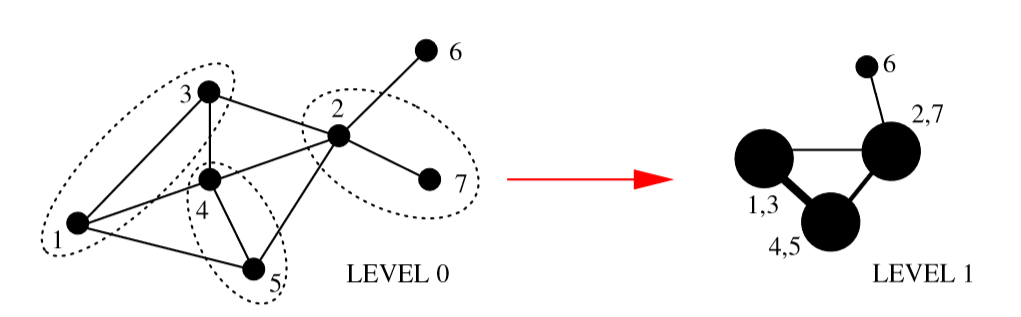
\includegraphics[width=.60\textwidth]{sag.png}
    \caption[SAG Coarsening]{SAG (strict aggregation) assumes a strict threshold per which it is determined whether two vertices should be coalesced or not \cite{coarsening}.}
    \label{fig:sag}
\end{figure}

\begin{figure}
    \centering
    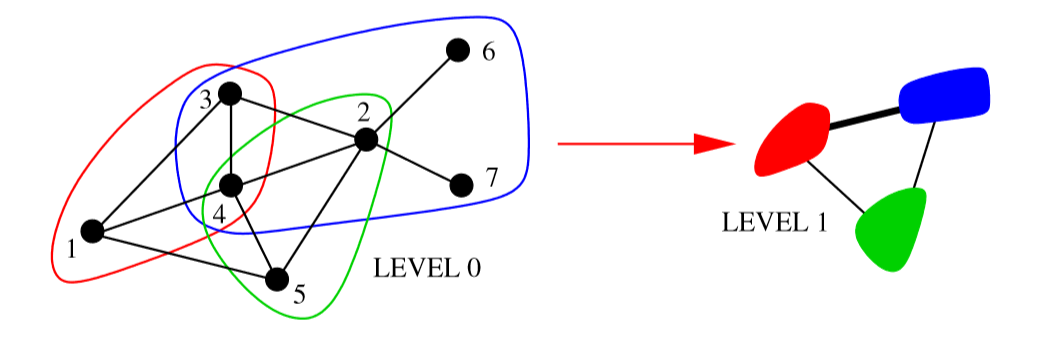
\includegraphics[width=.60\textwidth]{wag.png}
    \caption[WAG Coarsening]{WAG (weighted aggregation), in contrast to SAG, determines the \textit{likelihood} for different vertices to be clustered together, whereby vertices can be iteratively aggregated with further levels of coarsening \cite{coarsening}.}
    \label{fig:wag}
\end{figure}

Having discussed the specifics of the coarsening itself, we consider algorithms that specifically employ this technique. The main one that falls into this category is dubbed METIS, whose overall structure is as follows: ``The graph G is first coarsened down to a few hundred vertices, a bisection of this much smaller graph is computed, and then this partition is projected back towards the original graph (finer graph), by periodically refining the partition" \cite{metis}. In line with that, there are three main facets of this algorithm that necessitate discussion, specifically the coarsening, eventual clustering, and refinement of partitions during uncoarsening.

\begin{figure}
    \centering
    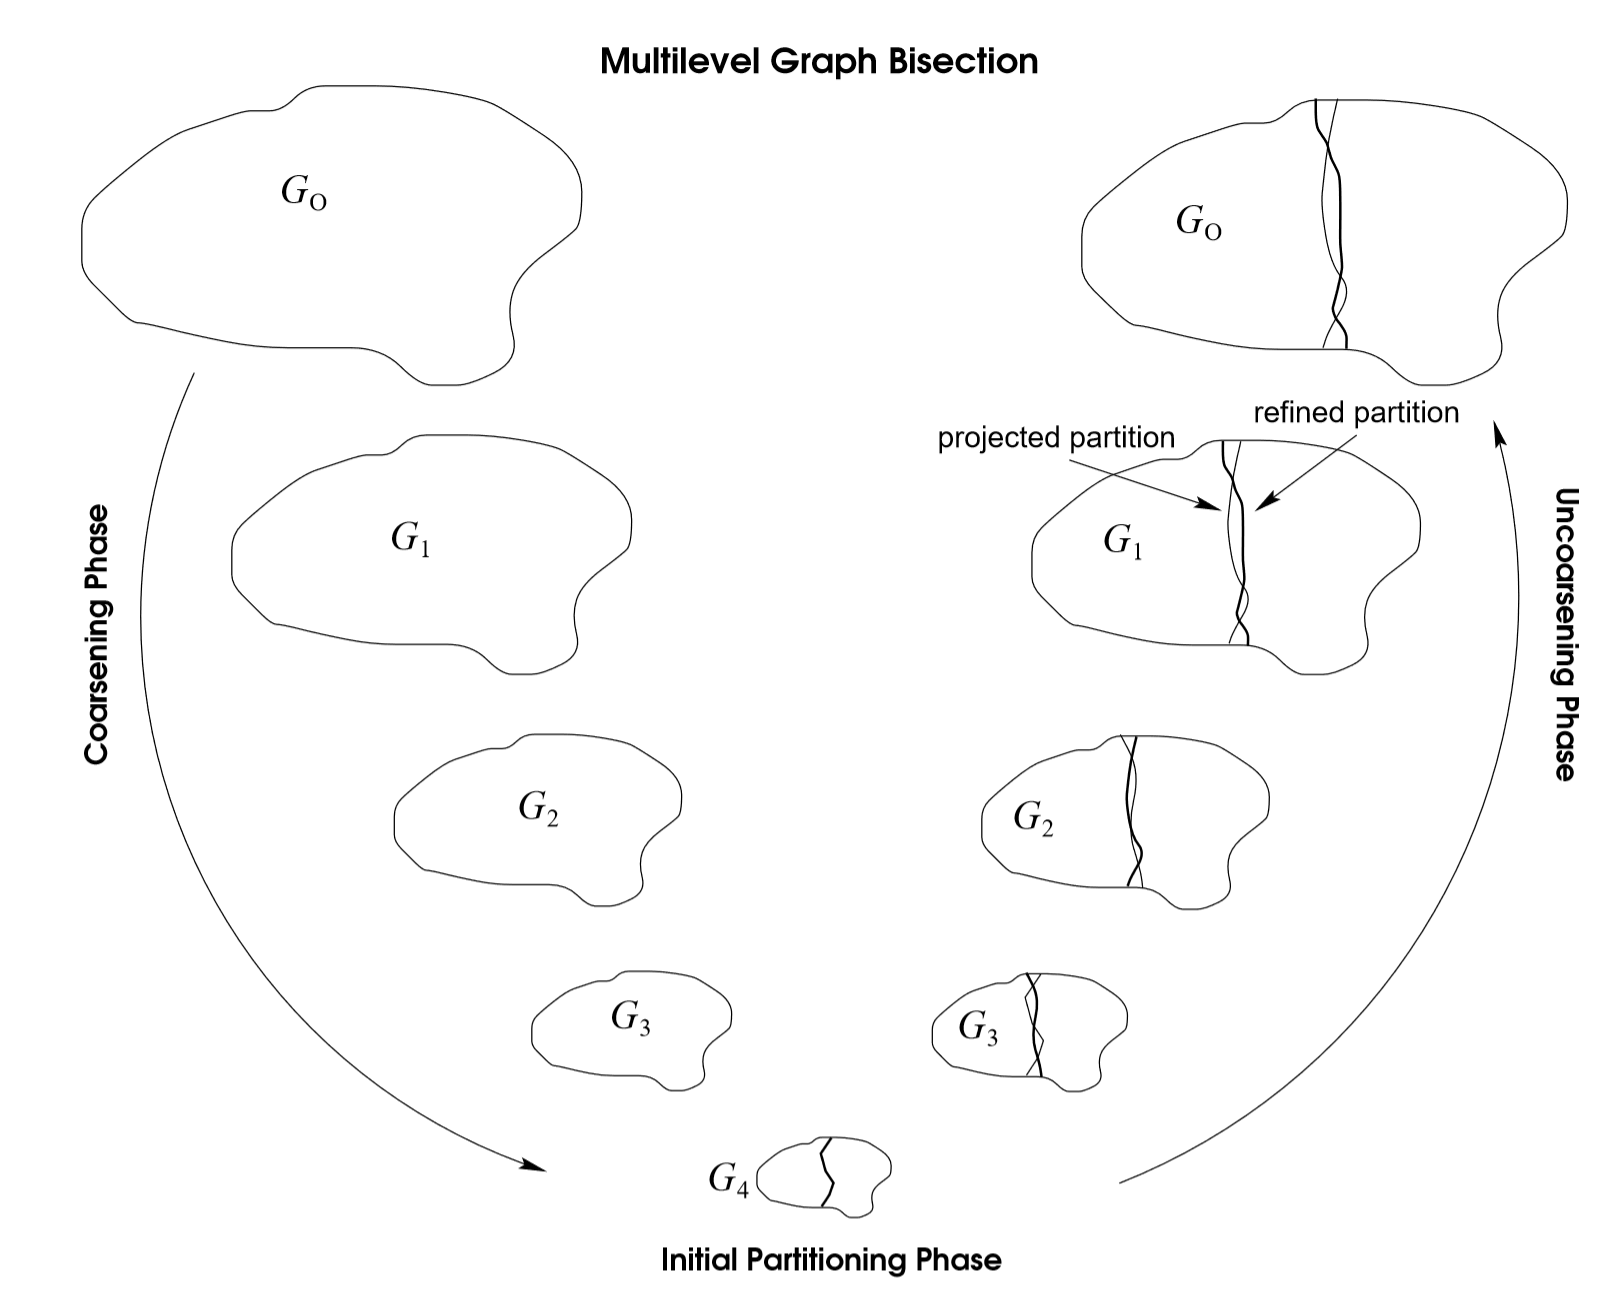
\includegraphics[width=.75\textwidth]{metis.png}
    \caption[METIS Architecture]{METIS relies on continual coarsening of the graph to a point where bisection or clustering is a relatively trivial problem and subsequently refining this partition as the graph is expanded back to its original size \cite{metis}.}
    \label{fig:metis}
\end{figure}

To be precise, the objective of the coarsening phase is to construct a sequence of graphs $\{G_{l}\}$ such that $|V_{l}| > |V_{l+1}|$, where we denote the original graph $G_{0}=(V_0,E_0)$ \cite{metis}. In line with this, ``$G_{l+1}$ is constructed from $G_l$ by finding a maximal matching $M_l\subset E_l$ of $G_l$ and collapsing together the vertices that are incident on each edge of the matching. In this process no more than two vertices are collapsed together because a matching of a graph is a set of edges, no two of which are incident on the same vertex" \cite{metis}. In line with the difference between SAG and WAG, there were multiple procedures discussed by which the maximal matching could be constructed, though it was found that the HEM ``heavy-edge matching..., [which] computes a matching $M_l$, such that the weight of the edges in $M_l$ is high...produces consistently better results than RM [random matching], and the amount of time spent in refinement is less than that of RM" \cite{metis}.

Having said that, we turn to the clustering section of the algorithm, referred to in Figure \ref{fig:metis} as the ``initial partitioning phase." Specifically, the algorithm supports ``four different schemes for partitioning the coarsest graph...Three of these algorithms are based on graph growing heuristics, and the other one is based on spectral bisection" \cite{metis}. For the purposes of this investigation, we decided to make use of spectral bisection, as this allowed for applying the results of experiments we conducted on the SBM initially. 

From here arises the main spectacle of the METIS algorithm: the uncoarsening phase. Formally, this involves taking the partitioning sets $\{C^k_i\}$ obtained in the coarsest level that satisfy $\bigcup_i C_i^l = V_k$ and projecting them up through $G_{k-1},G_{k-2},...,G_1,G_0$, such that each $\{C^l_i\}$ satisfies $\bigcup_i C^l_i = V_l$. In other words, taking the partitioning of the coarsest graph and attempting to efficiently construct a partitioning that eventually contains all the vertices of the original graph.

Towards that end, we can simply discuss how such a projection happens in a single step of the uncoarsening, from which the full process is fully defined. Specifically, a single step in this process begins with the natural projection up one level. That is to say, if two vertices $u,v$ were coalesced into a supernode $uv$ and said vertex $uv$ was clustered into class $A$, the natural projection simply assigns $u,v$ to $A$. However, ``even if the partition of $G_l$ is at a local minima, the projected partition of $G_{l-1}$ may not be at a local minima. Since $G_{l-1}$ is finer, it has more degrees of freedom that can be used to further improve the partition and thus decrease the edge-cut. Hence, it may still be possible to improve the projected partition of $G_{l-1}$ by local refinement heuristics" \cite{metis}. In other words, while it is the case that the clustering in the coarser level minimizes the crossing edges, this property is not necessarily retained in projecting up a level, due to the increased degrees of freedom. A ``refinement heuristic" here refers to one that takes ``two parts of the bisection [$A, B$ and]...selects $A'\subset A$ and $B'\subset B$ such that $A\backslash A' \cup B'$ and $B\backslash B' \cup A'$ is a bisection with a smaller edge-cut" \cite{metis}. The specific algorithm employed for this purpose was the Kernighan-Lin (KL) partition algorithm, though its details are not necessary to understand for our purposes.

In this way, METIS is capable of performing partitioning on enormous graphs, namely by creating a mapping from a large graph to a significantly reduced graph and one from this reduced graph's clustering to that of the original graph. 

\subsection{Notation}
Prior to delving into the experiments themselves, we present a comprehensive table of the notation introduced in the background sections for the purpose of serving as reference for the remainder of the paper. Note that the concepts presented in Table \ref{tab:notation} are clarified and more greatly discussed in their corresponding background section. 

\begin{table}[]
\centering
\caption[Mathematical Notation]{Notation/abbreviations as used in this paper unless otherwise noted}
\label{tab:notation}
\begin{tabular}{|l|l|}
\hline 
\textbf{Symbol} & \textbf{Interpretation} \\ \hline 
$G = (V,E)$ & Graph with vertices $V$ and edges $E$ \\\hline
$D$ & Graph degree matrix, i.e. degree of vertex $i$ in position $D_{ii}$ and 0 elsewhere \\\hline
$W$ & Graph weighted edge matrix \\\hline
$L$ & Graph Laplacian, defined as $L = D - W$ \\\hline
$\lambda_i$ & $i$th eigenvalue, when sorted in \textit{increasing} order, i.e. the $i$th smallest eigenvalue \\\hline
$v_i$ & $i$th eigenvector, i.e. the eigenvector associated with $\lambda_i$ \\\hline
$n$ & Number of nodes in the graph, i.e. $n=|V|$ \\\hline
$\{C_i\}$ & Graph clusters, such that $\bigcup_i C_i = V$, $\bigcap_i C_i = \emptyset$, $C_i \subset V$ \\\hline
$e_i$ & Standard $i$th basis vector of $\mathbb{R}^n$, i.e. $[0,0,\dots,1,0,\dots,0]$ (in position $i$) \\\hline
$SBM$ & Stochastic block model (planted partition model) \\\hline
$p,q$ & In- and out-cluster connection probabilities in SBM \\\hline
$NMI$ & Normalized mutual information \\\hline
$H$ & Entropy (probability/information theory) \\\hline
$F$ & Standard statistical F-score \\\hline
\end{tabular}
\end{table}

\clearpage
\section{Methodology}\label{methodology}
Having finished discussing the main relevant background, we turn to discussing the novel experiments/results conducted for this particular investigation. As was previously described, many of the results catered herein were performed on the SBM, from which relevant trends became apparent and their applicability to the full dataset more evident. Towards that end, the experiments are described here along with their intended purpose, and the associated results are presented in the corresponding subsection of Section \ref{results}.

\subsection{SBM Clustering Trial}
Given that the objective of this investigation is to perform a clustering on the full-scale heuristics graph, the main goal of these lead-up experiments was to ascertain which of the clustering techniques discussed in the background would be best suited for our purposes. Thus, this first experiment, as with all that follow, involved taking three metrics and assigning a cumulative score to each technique. Specifically, the three metrics were those defined in the Section \ref{evaluation}, namely the purity, normalized mutual information, and F-score (weighted rand index). Of course, the cumulative score was proportional to each of the three accuracy metrics, though weights were assigned on the basis of what was of greatest importance for our purposes. Thus, the final ``evaluation score" is:

\begin{align}
    score = \frac{w_{purity}purity + w_{NMI}NMI + w_{F}F}{w_{purity} + w_{NMI} + w_{F}}\label{eq:overall}
\end{align}

The specific algorithms that were tested against one another in this section will be all the offline and out-of-box (i.e. previously implemented) algorithms discussed, namely: hierarchicial spectral, k-means spectral, spectral (\texttt{scikit-learn}), k-means (\texttt{scikit-learn}), DBSCAN (\texttt{scikit-learn}), and METIS. Thus, the outputs of this section include the following:

\begin{enumerate}
    \item \textbf{Metric plots:} For each of the three metrics in addition to the cumulative score, plots of performance by the different clustering algorithms for given fixed values of $p$ (as defined in the SBM) over varying levels of $q$. 
    \item \textbf{Time plot:} Each of the clustering algorithms were run on fixed choices of $p,q$ while varying the size of the graphs, for which the time for completion of the clustering are plotted.
    \item \textbf{Sample clustering:} The graphs themselves, after clustering was performed, are provided for sake of understanding the nature, in terms of strengths and weaknesses, of the different clustering algorithms.
\end{enumerate}

Thus, it was the intention of this section to have a clear choice for an algorithm to be used for clustering on the final heuristics graph.

\subsection{SBM Sparsification Trial}
In addition to the offline algorithms, there were the variations discussed in the background section to see if approximation techniques could be employed for the purposes of rendering time expended while retaining reasonable accuracy. Amongst these was sparsification, which we wished to empirically analyze in the same fashion as described in the above section, namely testing out its performance against various metrics on the SBM. Thus, we tested the performance of spectral sparsification of the two manually implemented spectral clustering algorithms. It was expected that sparsification would result in a slight degradation of accuracy, though ideally non-significant, and a decrease in computation time.

\subsection{SBM Coarsening Trial}
In addition to the sparsification, coarsening was tested against the vanilla clustering algorithms. This coarsening trial, however, was somewhat redundant from the previous experiment, as METIS is itself a coarsening algorithm at heart. We, therefore, anticipated that performance, although potentially superior to other vanilla algorithms, would be of lower quality than METIS, though certain trends or observations would be more parseable through this trial than can be scrutinized from the black-box algorithm that is METIS.

\subsection{SBM Online Trial}
The final portion of this optimization was ascertaining the effectiveness of online clustering techniques. In particular, we sought to implement and test the relative performance of evolutionary spectral algorithms when given little weight to temporal smoothness. Of course, in line with that, we anticipated the main advantage of such online trials would come in the lower need for memory consumption, meaning the score defined hereto would seemingly not account for this benefit. While this is the case, this was fully intentional, as the cost of memory is significantly outweighed by that of time. If, however, memory is of concern for future researchers, it may be of interest to factor this aspect into the score, potentially measuring such aspects by \texttt{top} or \texttt{/proc/meminfo} with respective to the appropriate pid. All in all, however, these four aforementioned experiments were ideally intended to result in there being one algorithm, whether it be offline, online, using sparsification, or coarsening, that performs best across all metrics to be used in the final dataset trial. 

\subsection{Full Dataset Trial}
With the final determined algorithm, trials were conducted on both partial datasets in addition to the full dataset, with emphasis being placed on its performance agaisnt the known ground truth. Thus, accuracy was measured by the same metrics as defined above except only on a subset of the full dataset. Presented as a result from this were the clustered results (similar to Figure \ref{fig:fistful}) and the accuracy metrics as a table.

\clearpage
\section{Results}\label{results}
We present the figures and tables as elaborated in the previous section in the following subsections. This section was the result of running the code available at \url{https://github.com/yashpatel5400/anonychain}, as described more fully in that repo (written in Python 3). The relevant discussion, i.e. interpretation of the figures, are given in the following section, namely Section \ref{discussion}.

For specifics on how the trials were run, we provide the summary below:
\begin{itemize}
    \item \textbf{SBM Clustering:} For multiple values of $p$, i.e. holding $p$ fixed, we chose a corresponding set of values of $q$ to run trials on. For each pair $(p,q)$, five identical trials were run. Each trial produced an SBM using these values of $p,q$. From here, each of clustering algorithms were run and their accuracies, across all metrics, and times were measured. After the five trials were run, an average score was computed, thus leaving a single data point per metric corresponding to the pair $(p,q)$ across the various algorithms. After being computed over all relevant values of $p,q$, the values were plotted. Note that, across all the trials, the following were the cluster sizes used: \texttt{[63,53,32,25,20,18,14,12,8,7,7,5,4,3,3,2]}. These somewhat arbitrary sizes were chosen, as they roughly correspond to the heuristics graph nature, where a small subset of the graph has a large portion of the wallets (i.e. Coinbase and Mt. Gox) and the remainder have a reasonable number. In addition, the overall score was computed with $w_{purity}=1.0,w_{NMI}=3.0,w_{F}=2.0$. These particular values of weights were chosen as NMI most closely captures the notion of determining the ``overlap" with the underlying clusters while also penalizing separating vertices into their own compartments. 
    \item For clarity, the labels as associated with the various clustering algorithms are laid out below:
    \begin{itemize}
        \item \textbf{KMeans}: Standard k-means algorithm, as implemented in \texttt{scikit-learn}
        \item \textbf{ManualHierarchical}: A manually implemented hierarchical spectral clustering algorithm, i.e. based on the principle of spectral bisection
        \item \textbf{ManualKMeans}: A manually implemented k-means spectral clustering algorithm, i.e. one which performs the final clustering on graph in a single iteration
        \item \textbf{METIS}: METIS algorithm as described in Section \ref{coarsening-bg}
        \item \textbf{MiniBatchKMeans}: Mini-batch k-means algorithm, a modified implementation of the k-means algorithm, which seeks ``to reduce the computation time, while still attempting to optimise the same objective function. Mini-batches are subsets of the input data, randomly sampled in each training iteration. These mini-batches drastically reduce the amount of computation required to converge to a local solution. In contrast to other algorithms that reduce the convergence time of k-means, mini-batch k-means produces results that are generally only slightly worse than the standard algorithm" \cite{scikit}
        \item \textbf{SpectralClustering}: Spectral clustering algorithm, as implemented in \texttt{scikit-learn}
    \end{itemize}
    \item Coarsening was implemented much in the way it is in METIS. That is to say, rather than arbitrarily selecting edges, a matching of maximal weight was determined and used for the purposes of edge contraction. From there, the clustering was performed, and clustering results expanded to the original graph. As the purpose of this particular subset of experimentation was to tease out information regarding the loss in accuracy relayed by clumping nodes, no additional ``refinement algorithm" was implemented, as is done in METIS. Instead, we simply expand the projected partition to the original graph as our final result. In addition, performing multiple levels of matching simply involved repeated edge contraction, clustering, and a direct expansion to the original graph, rather than the stepwise uncoarsening process employed by METIS.
    \item Any visualization of the graphs/network structure was completed using the standard Fruchterman-Reingold force-directed algorithm, as implemented by the Python NetworkX package. Briefly, the algorithm revolves around associating between each pair of vertices a ``spring" which pulls them in accordance to their connection (edge) weight together against a repulsive force experienced mutually between all vertices \cite{graph-viz}.
    \item Unlike the previously described trial averaging method, the structure for the sparsification trials was simply varying the $\varepsilon$ parameter while fixing a value of $p,q$ and conducting a single trial per chosen parameter value. This was specifically done as, unlike accuracy metrics, which vary significantly on the basis of random variations in the formation of the SBM graph, the time necessary to execute an algorithm remains relatively constant on the basis of the graph size. While there are variations associated with random initializations of some algorithms, such as k-means, these were not in the sparsification section, rendering this a non-issue.
\end{itemize}

\subsection{SBM Clustering Results}
\begin{figure}[H]
    \centering
    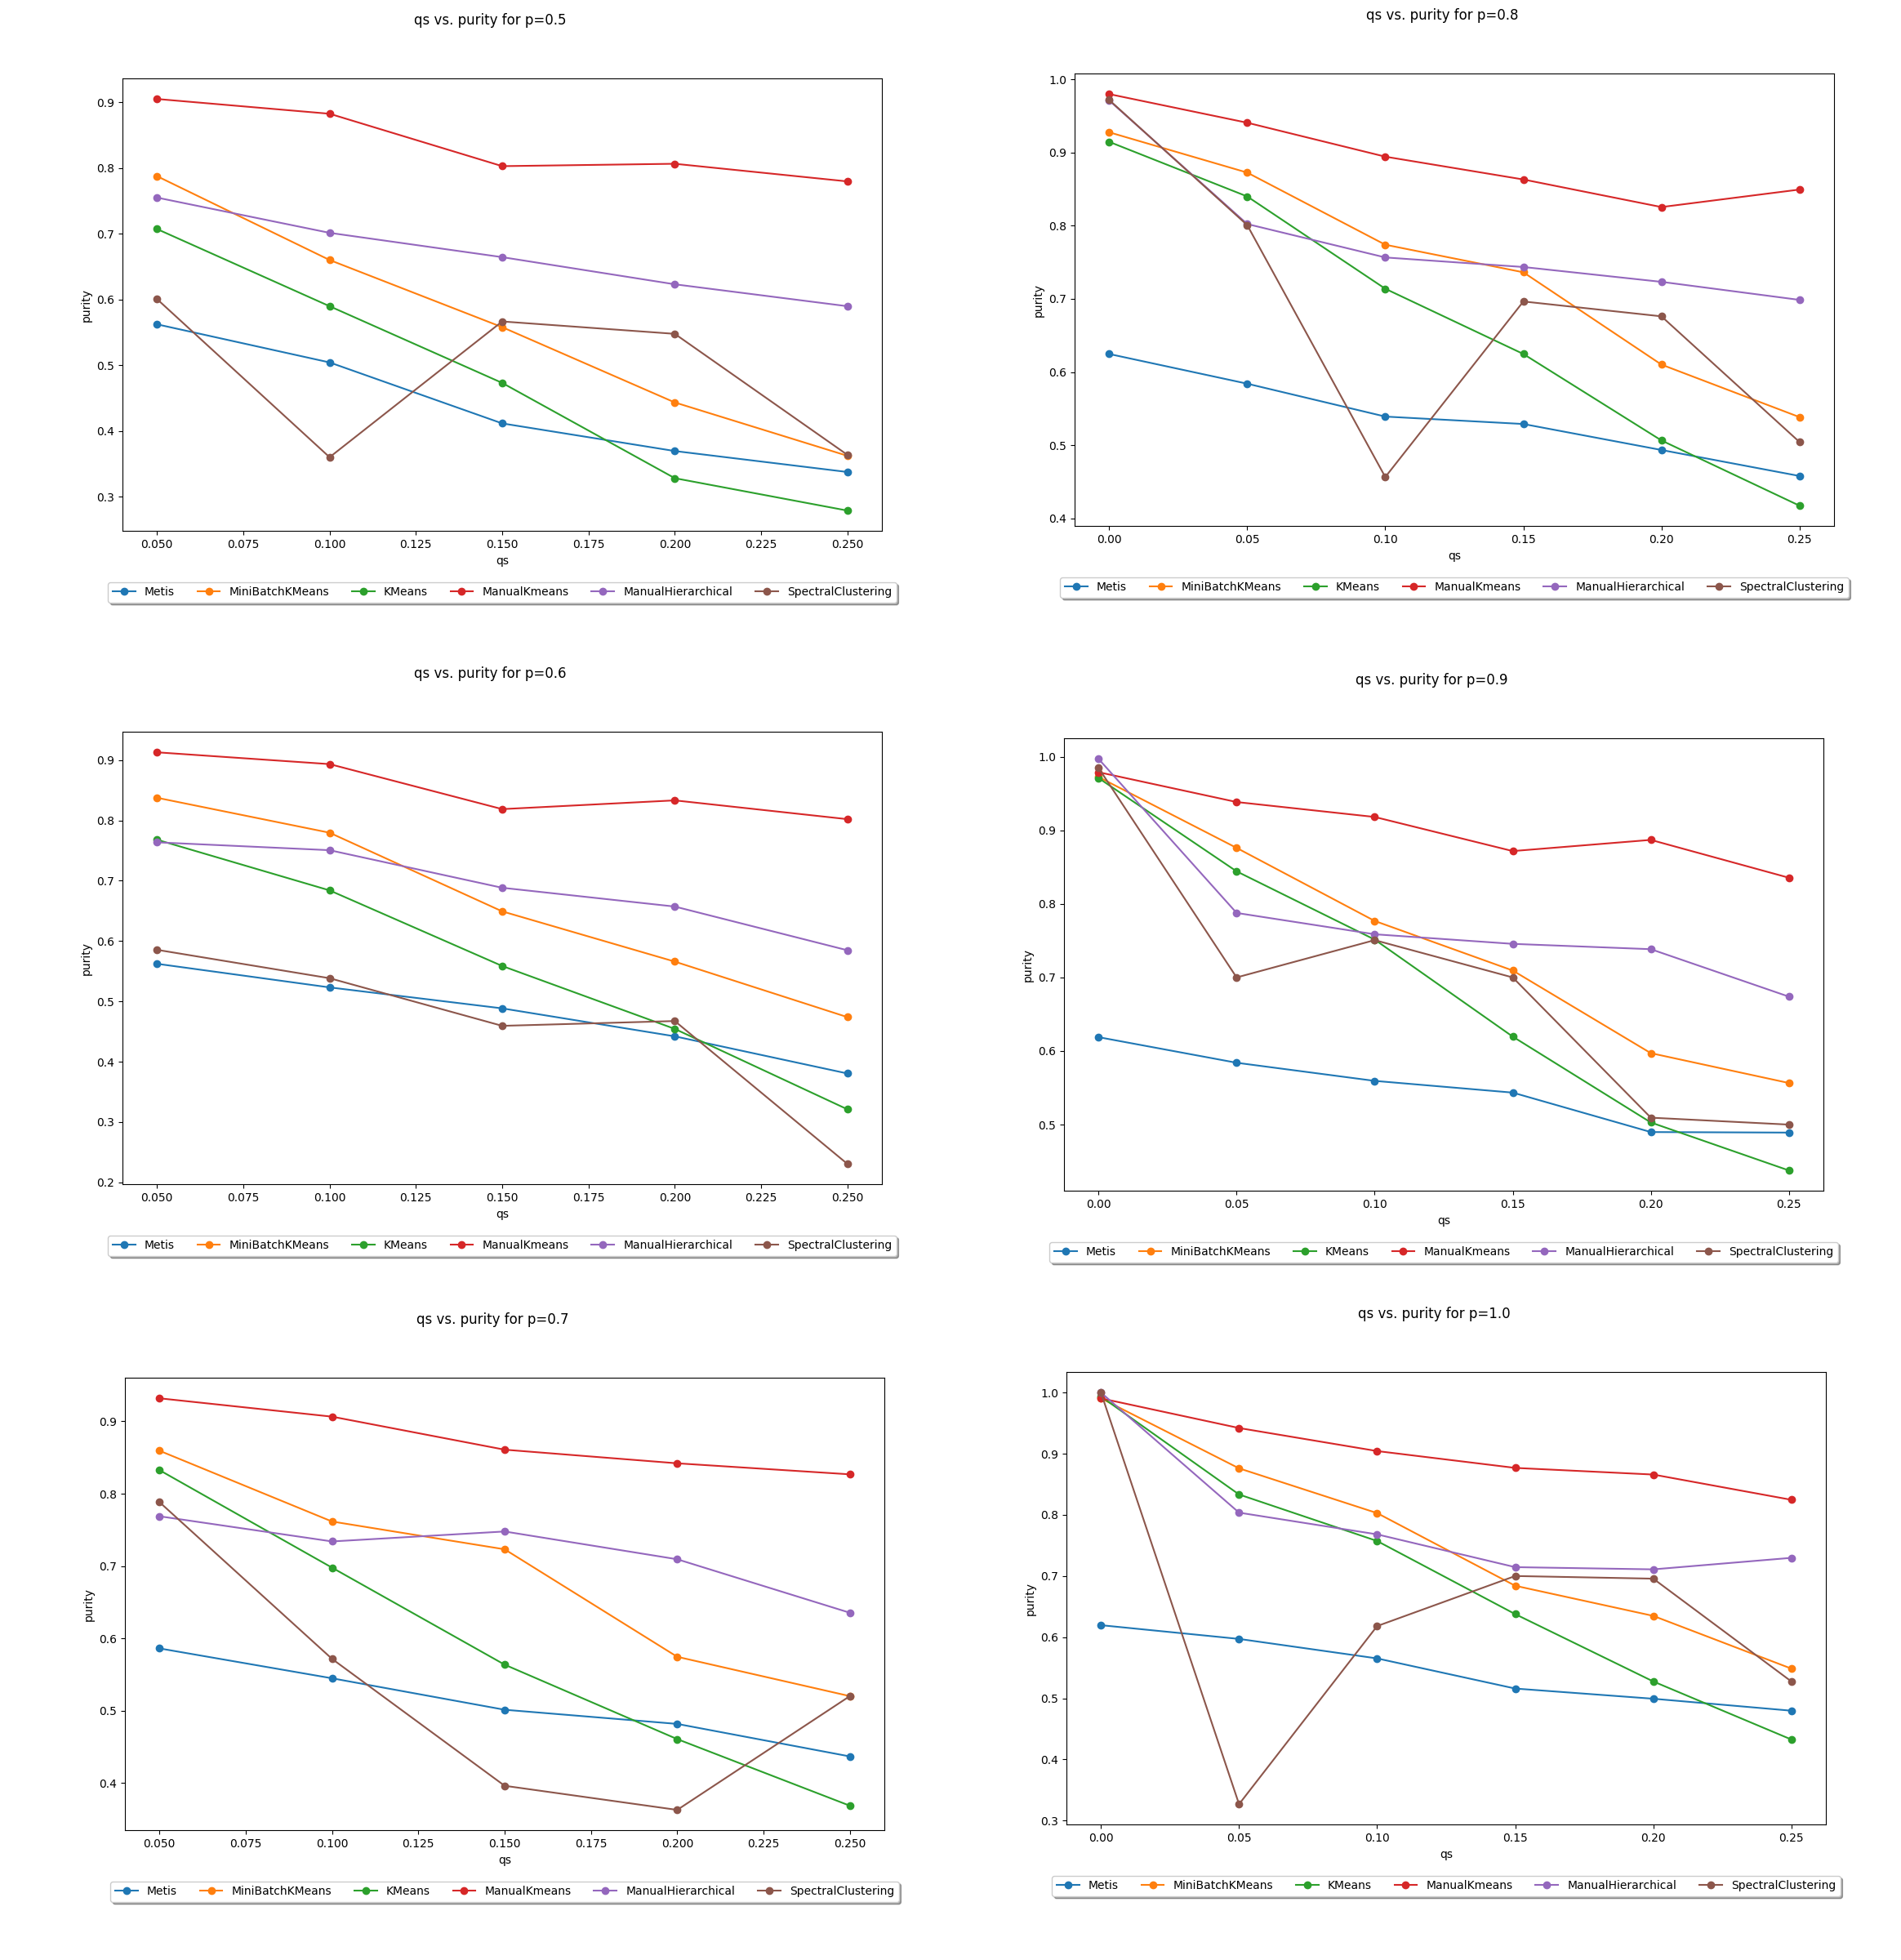
\includegraphics[width=1.15\textwidth]{results/results_purity.png}
    \caption[Clustering purity results]{Results of running the clustering algorithms for the purity metric. The $p$ values go from $p=0.5$ to $p=1.0$ in increments of $0.1$, increasing down the columns.}
    \label{fig:results_purity}
\end{figure}

\begin{figure}[H]
    \centering
    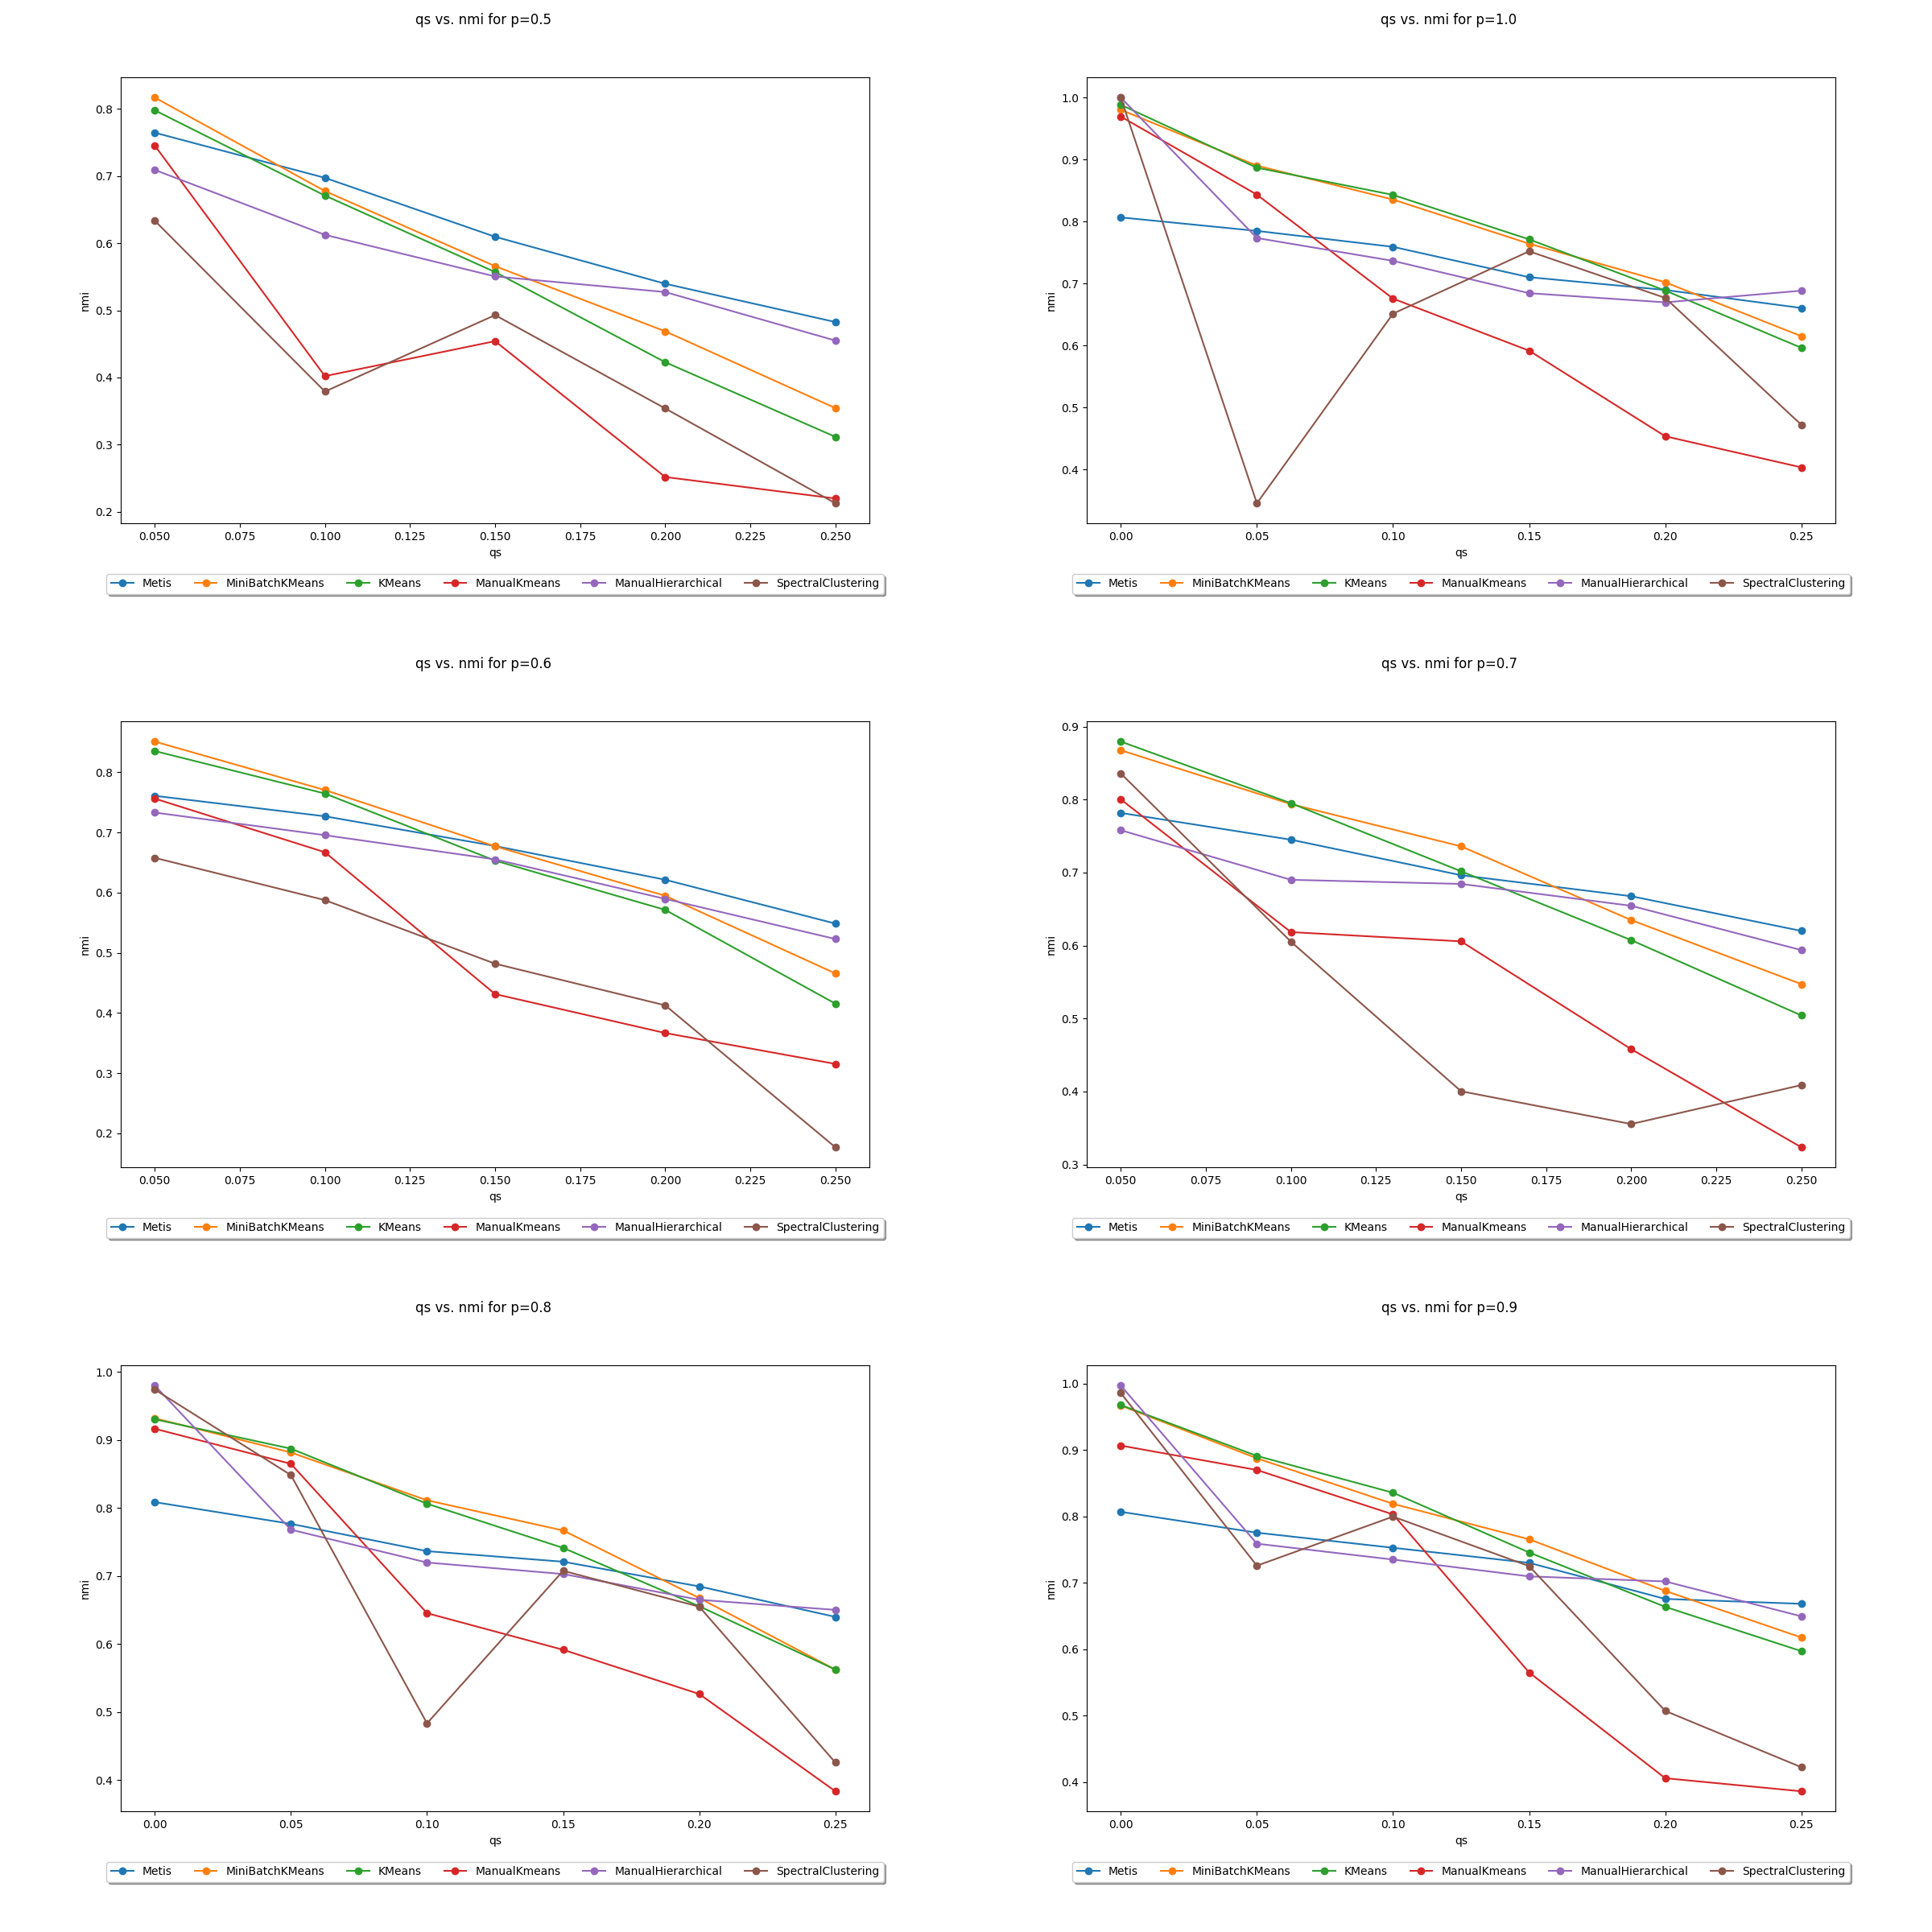
\includegraphics[width=1.15\textwidth]{results/results_nmi.png}
    \caption[Clustering NMI results]{Results of running the clustering algorithms for the NMI metric. The $p$ values go from $p=0.5$ to $p=1.0$ in increments of $0.1$, increasing down the columns.}
    \label{fig:results_nmi}
\end{figure}

\begin{figure}[H]
    \centering
    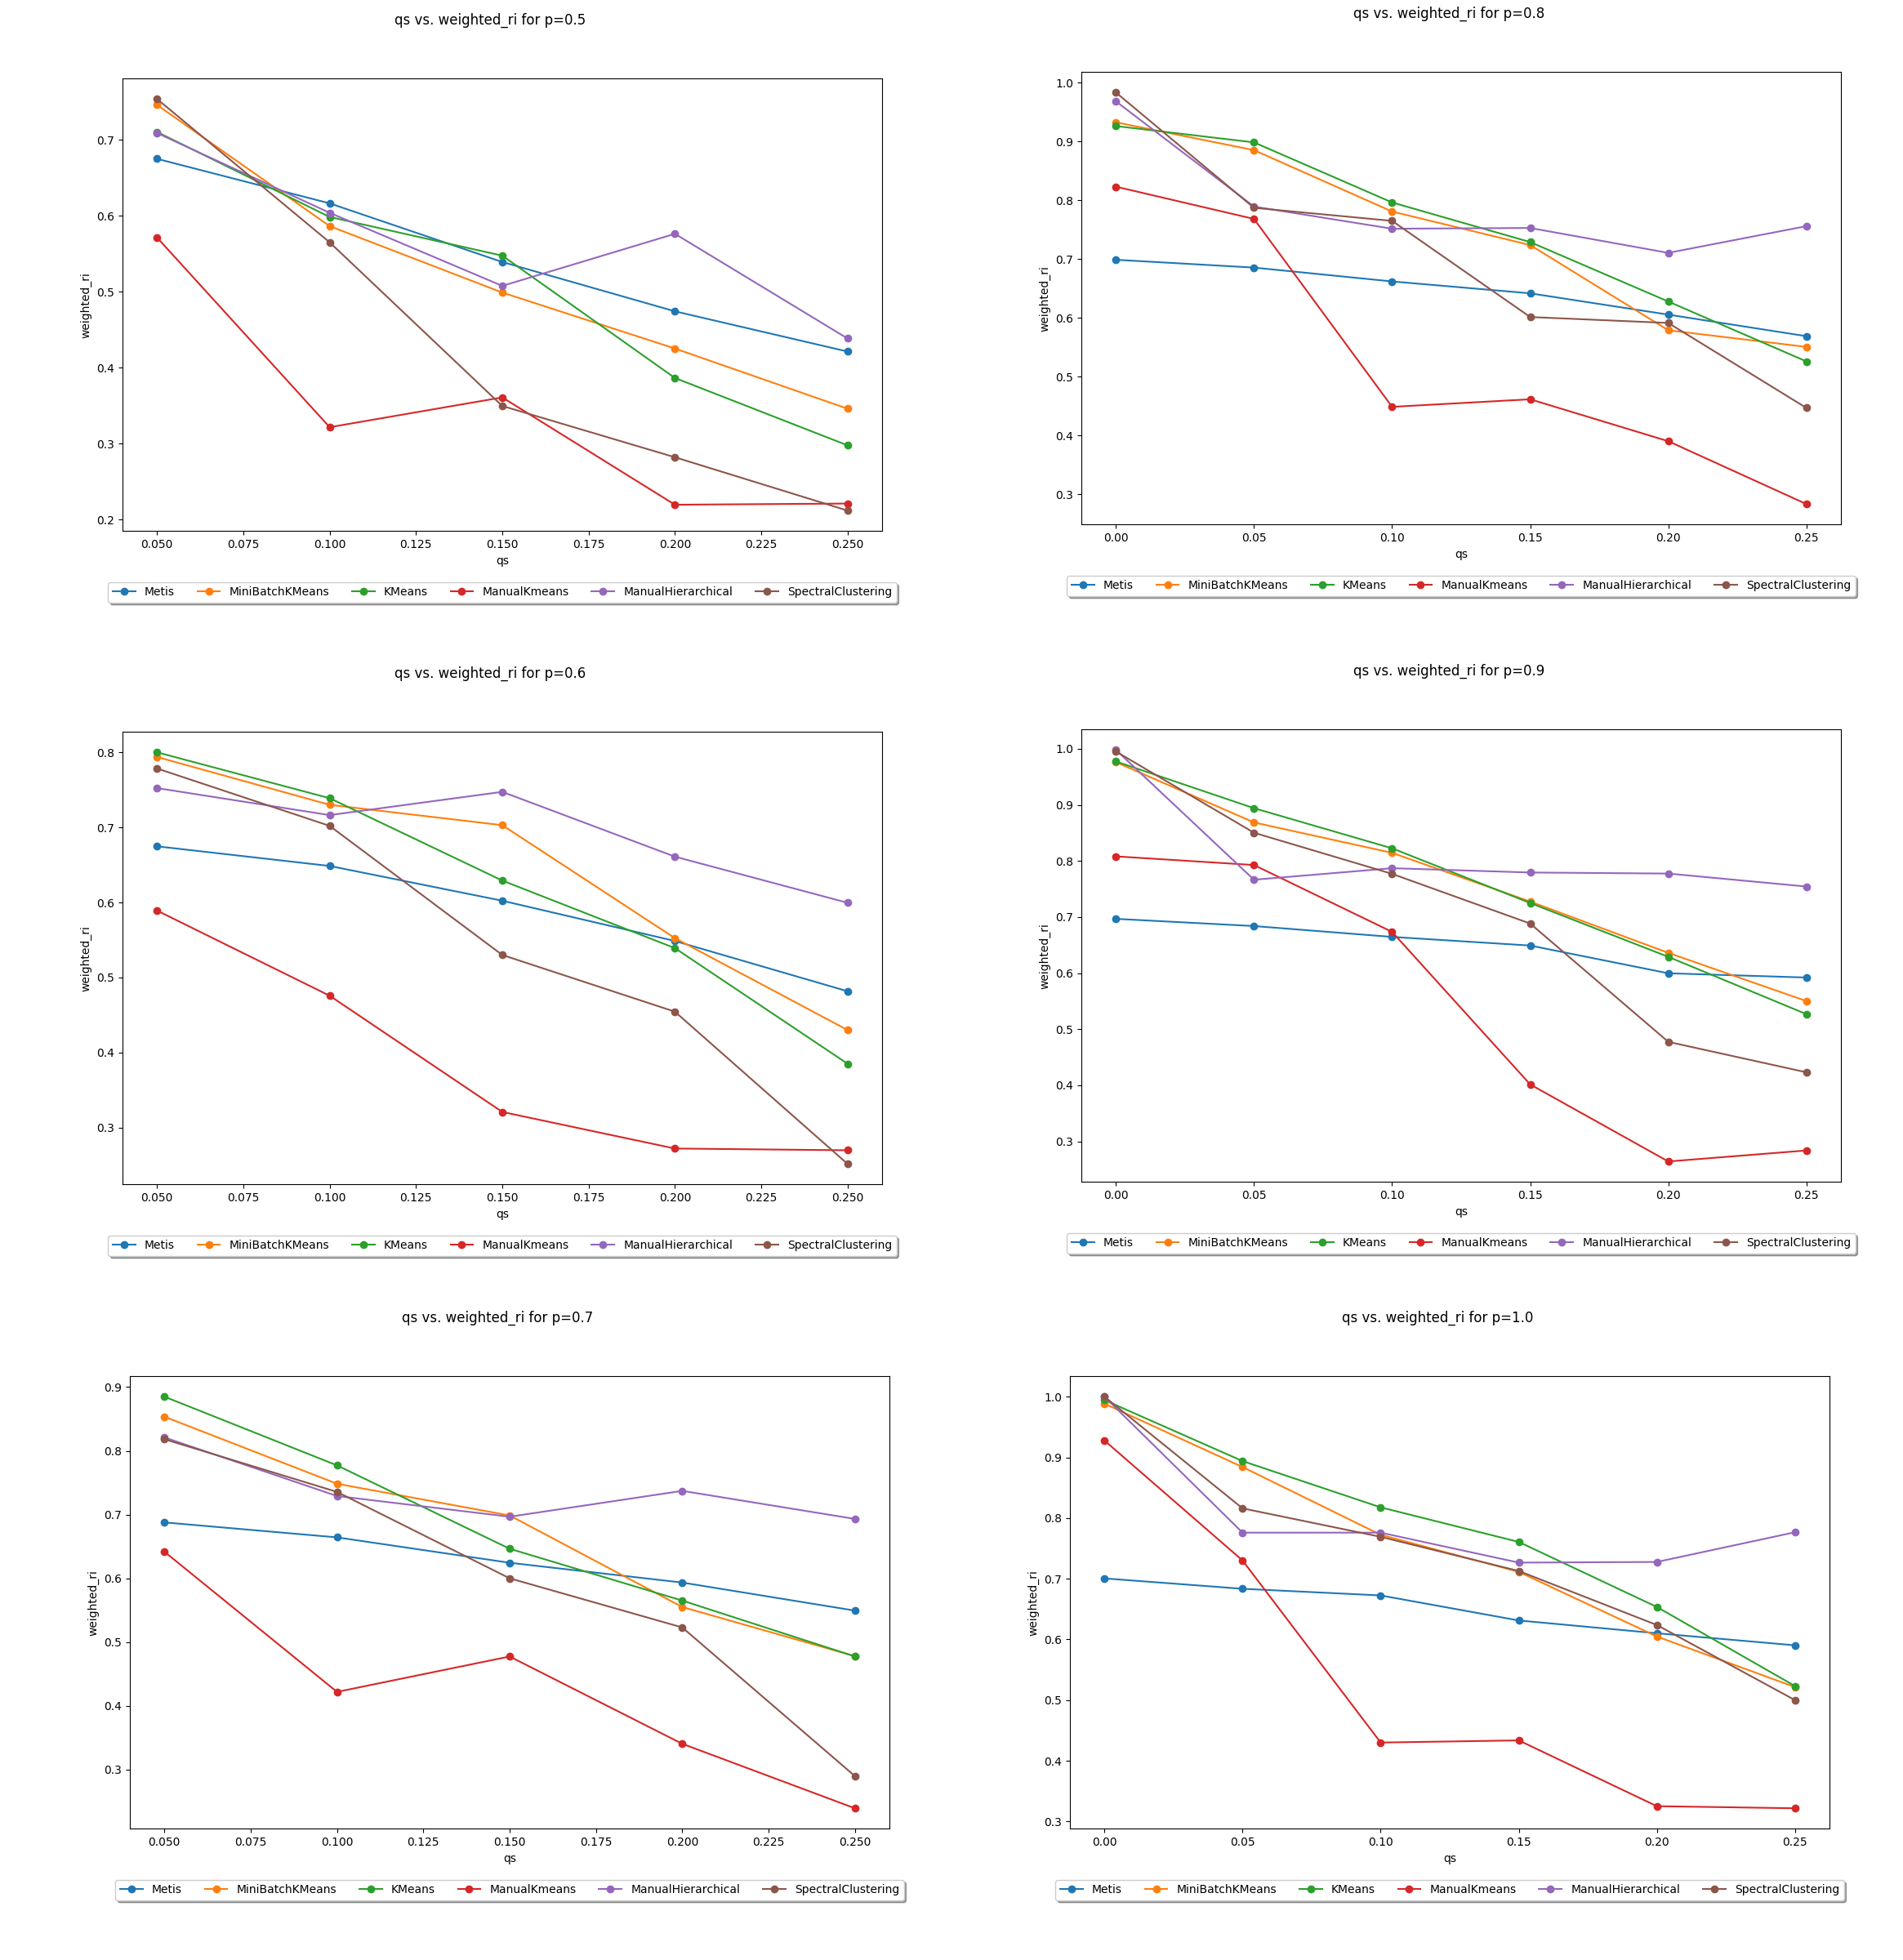
\includegraphics[width=1.15\textwidth]{results/results_weighted_ri.png}
    \caption[Clustering weighted RI (F-score) results]{Results of running the clustering algorithms for the F-score metric. The $p$ values go from $p=0.5$ to $p=1.0$ in increments of $0.1$, increasing down the columns.}
    \label{fig:results_weighted_ri}
\end{figure}

\begin{figure}[H]
    \centering
    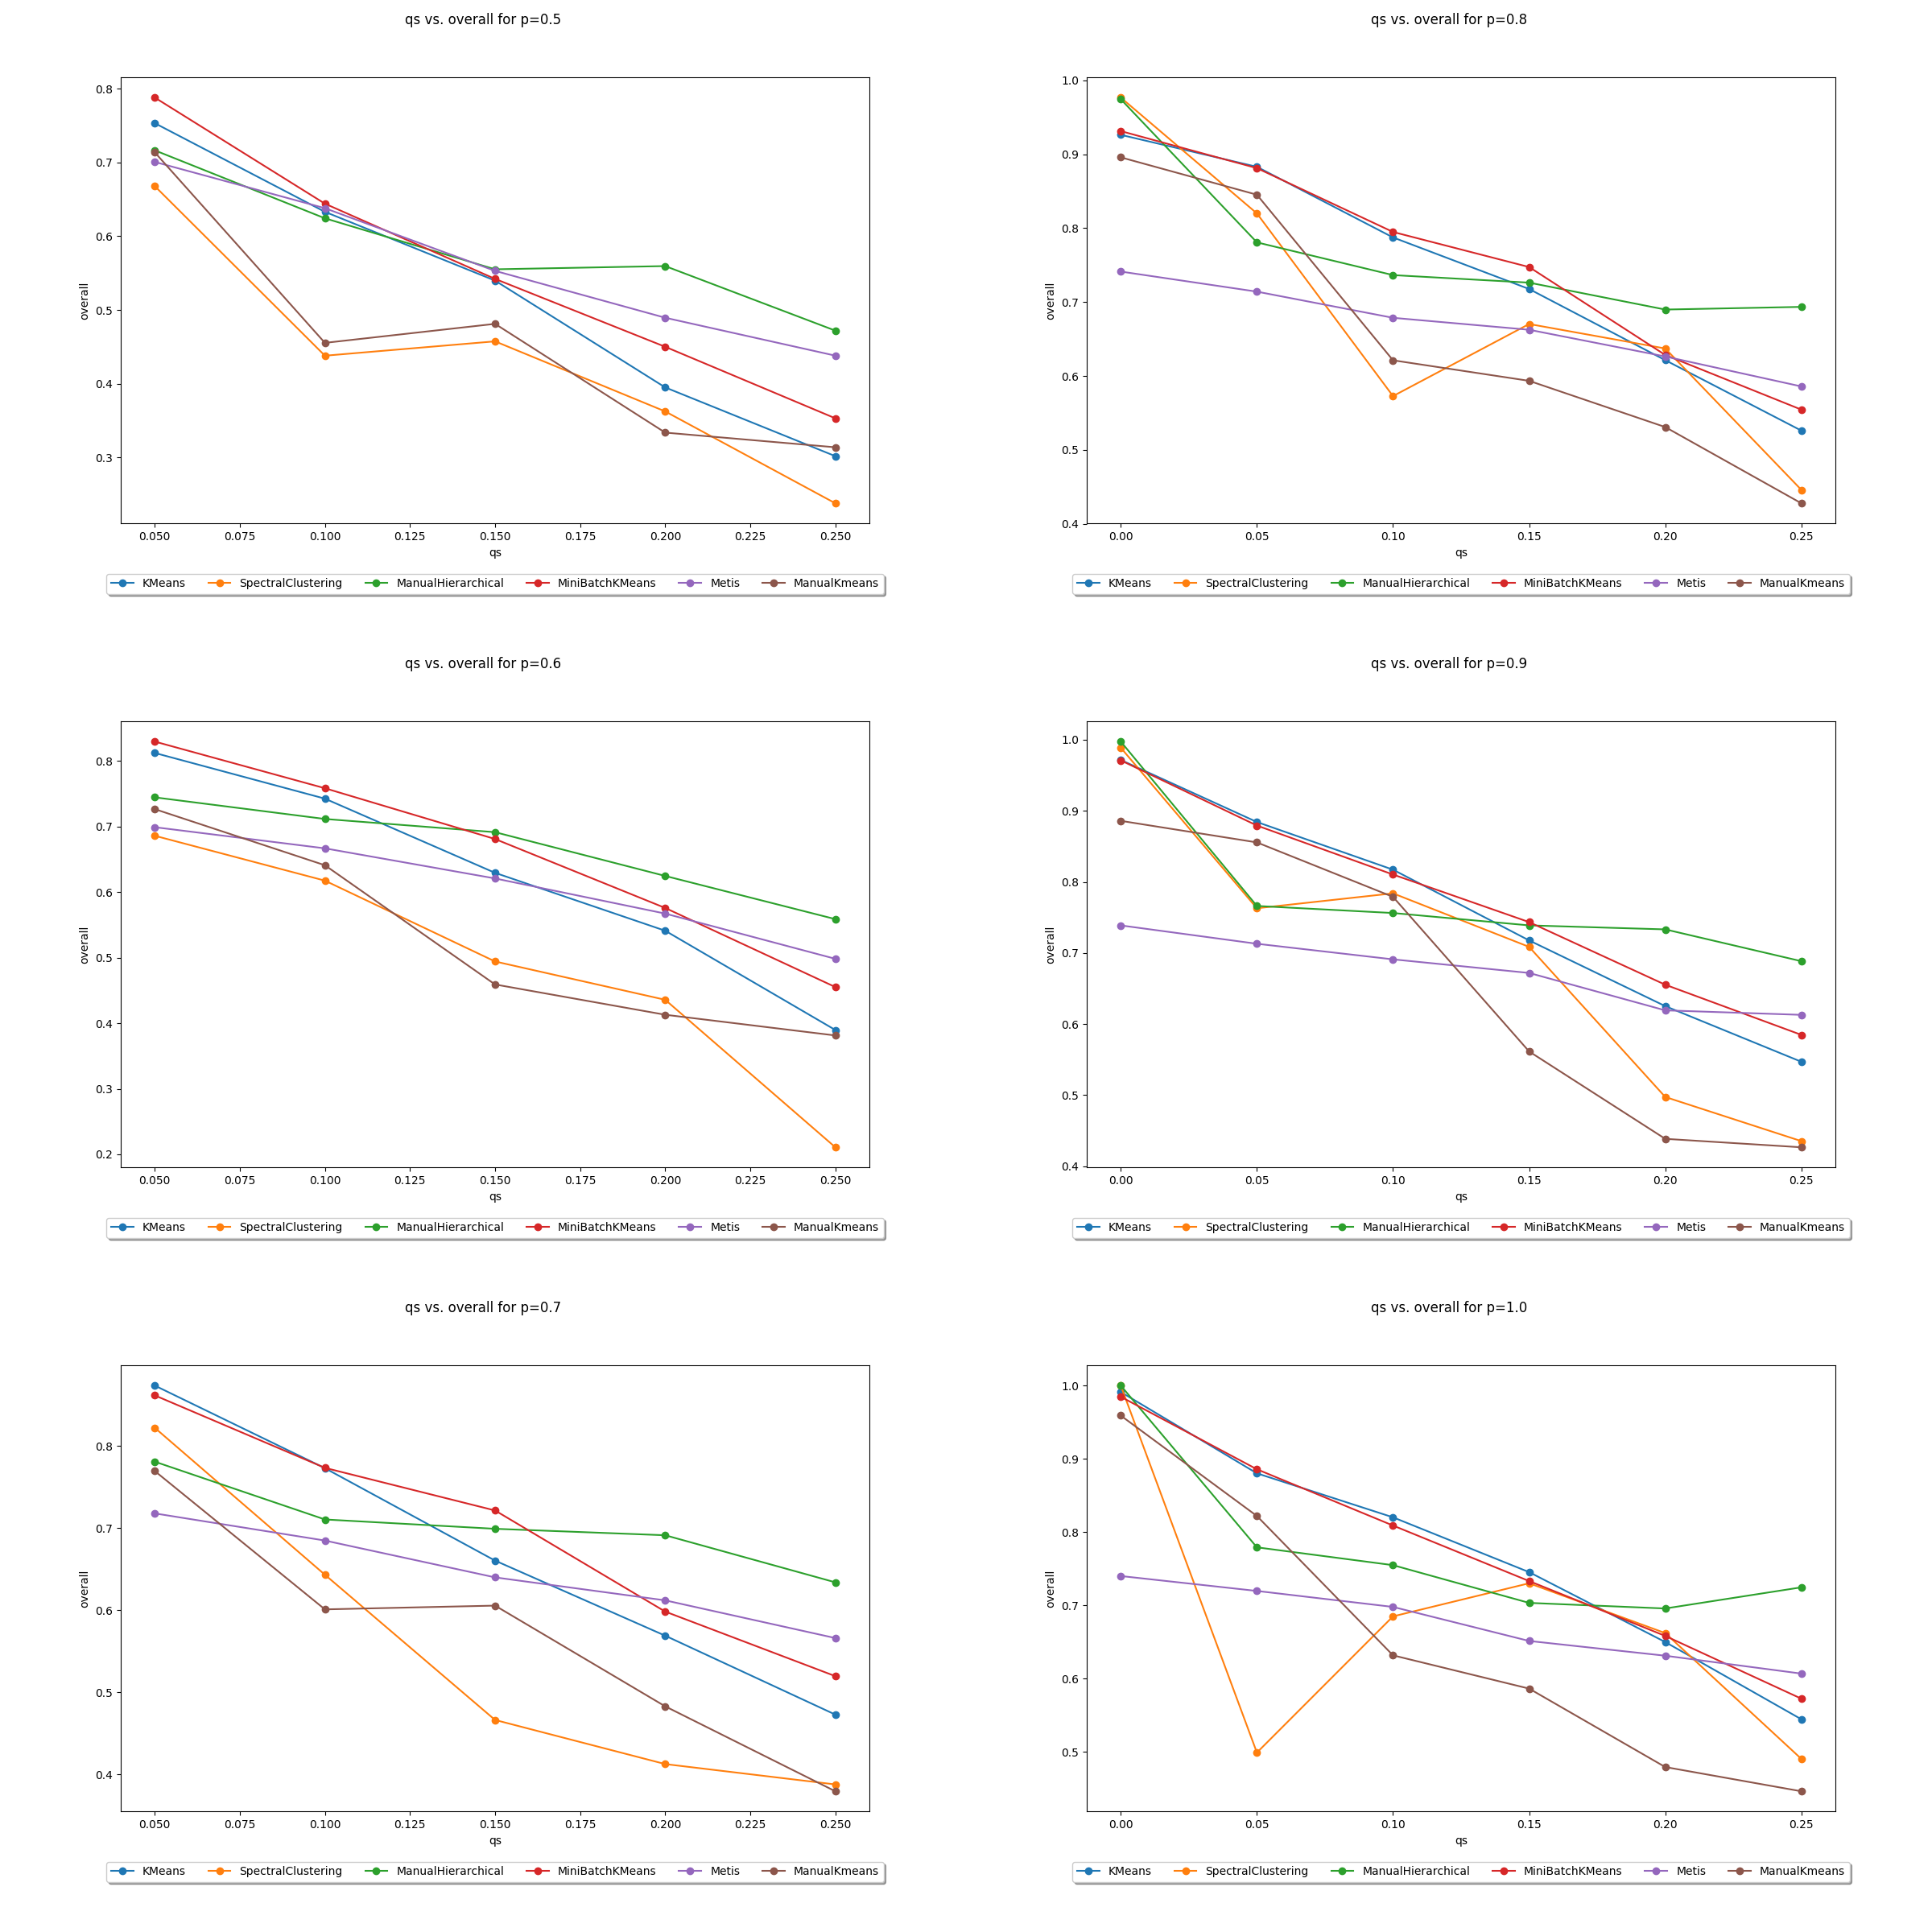
\includegraphics[width=1.15\textwidth]{results/results_overall.png}
    \caption[Clustering overall score results]{Results of running the clustering algorithms for the overall score metric, as defined by Eqn. (\ref{eq:overall}), where we specifically elected to use $w_{purity}=1.0, w_{NMI}=3.0,w_{F}=2.0$. The $p$ values go from $p=0.5$ to $p=1.0$ in increments of $0.1$, increasing down the columns.}
    \label{fig:results_overall}
\end{figure}

\begin{figure}[H]
    \centering
    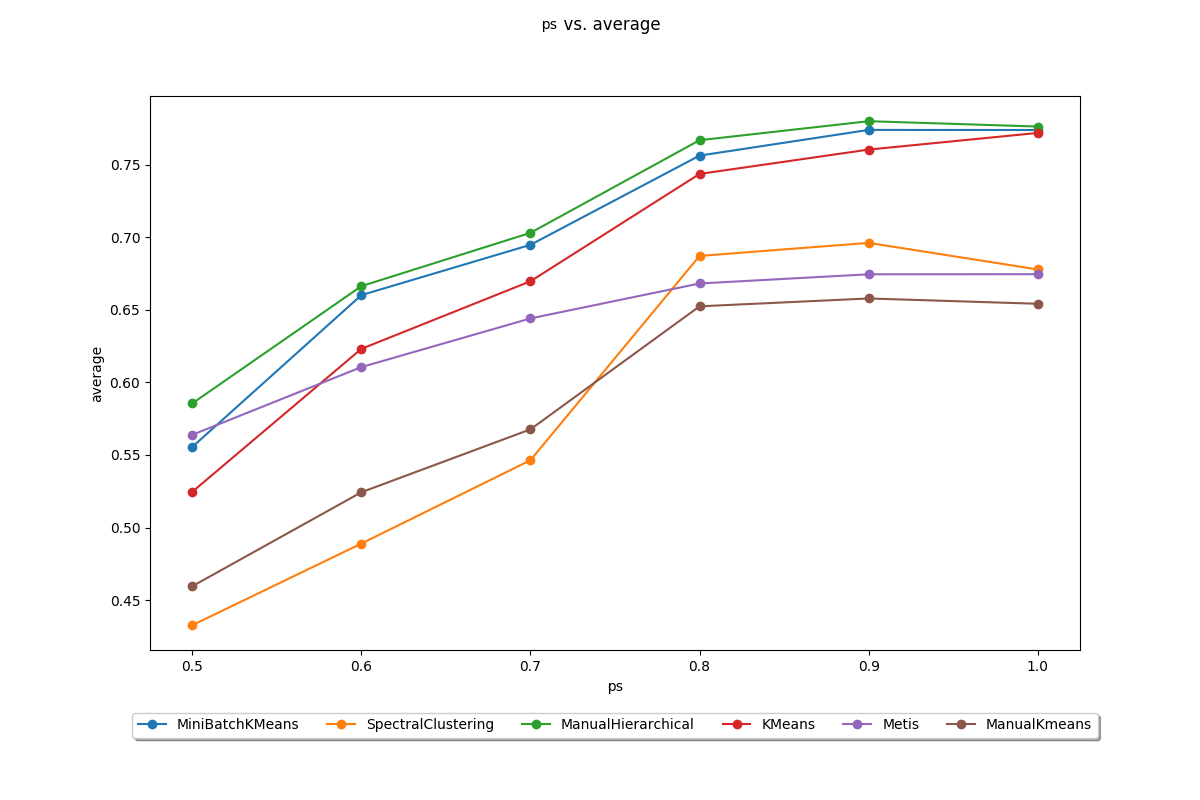
\includegraphics[width=1.0\textwidth]{results/results_average.png}
    \caption[Clustering average overall score across $p$]{For each of the $p$ trials in Figure \ref{fig:results_overall}, we averaged the overall scores across the different values of $q$, plotted here.}
    \label{fig:results_average}
\end{figure}

\begin{figure}[H]
    \centering
    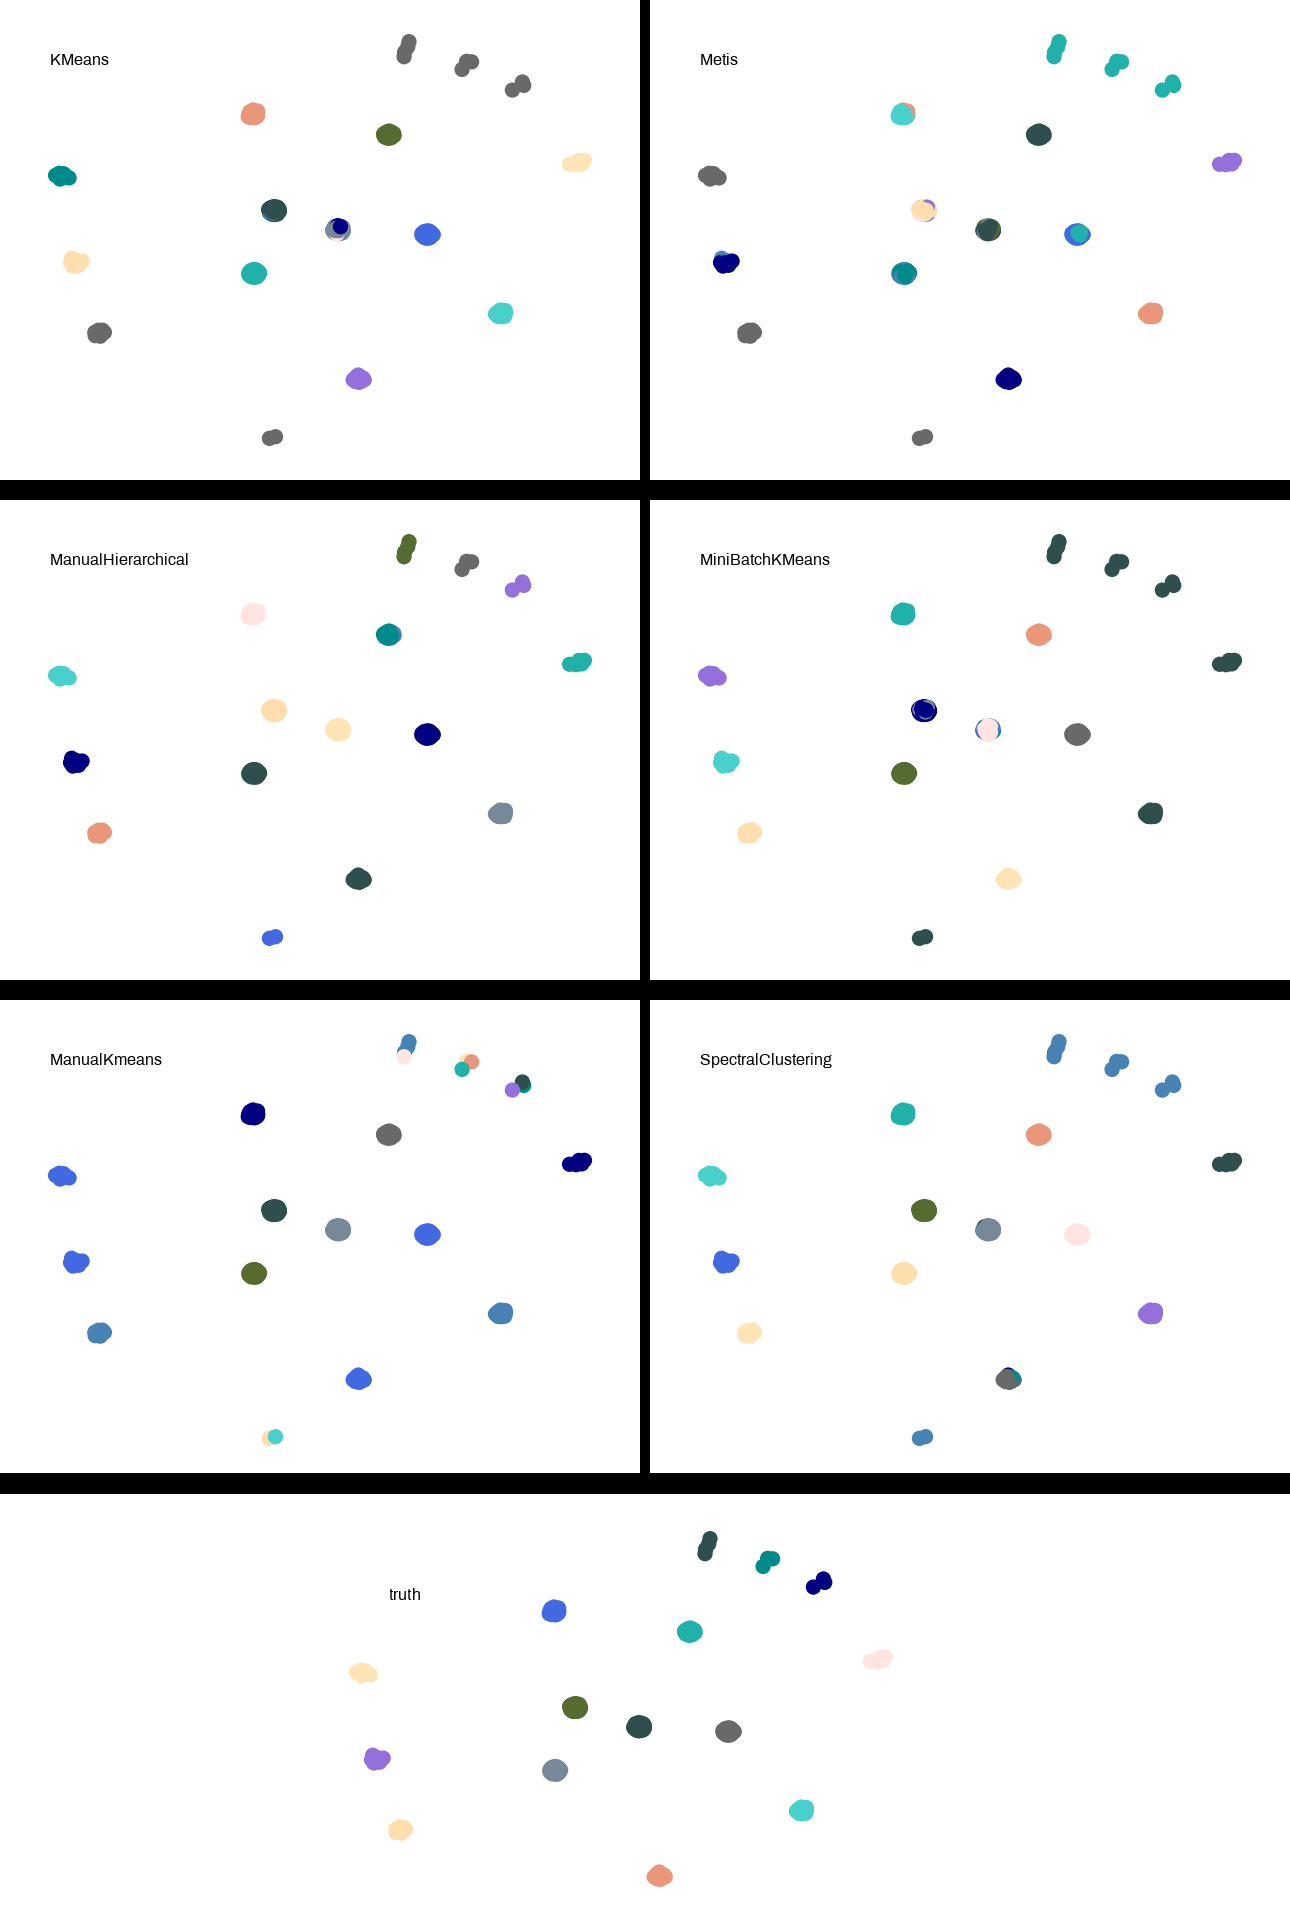
\includegraphics[width=.85\textwidth]{results/results_p-80_q-00.png}
    \caption[Clustering for $p=0.80,q=0.0$]{Clustering results for $p=0.80,q=0.0$, where the performed clustering is annotated in the top-left corner and the ground truth provided at the bottom. Clearly, while the colors within a particular clustering are consistent, it means nothing to compare these colors across clusterings as labelling one group $A$ and another $B$ is wholly arbitrary and just as valid vice versa. Of note is that all algorithms performed quite well here, namely in the circumstance where the clusters are well-separated (i.e. $q=0$).}
    \label{fig:results_p-80_q-00}
\end{figure}

\begin{figure}[H]
    \centering
    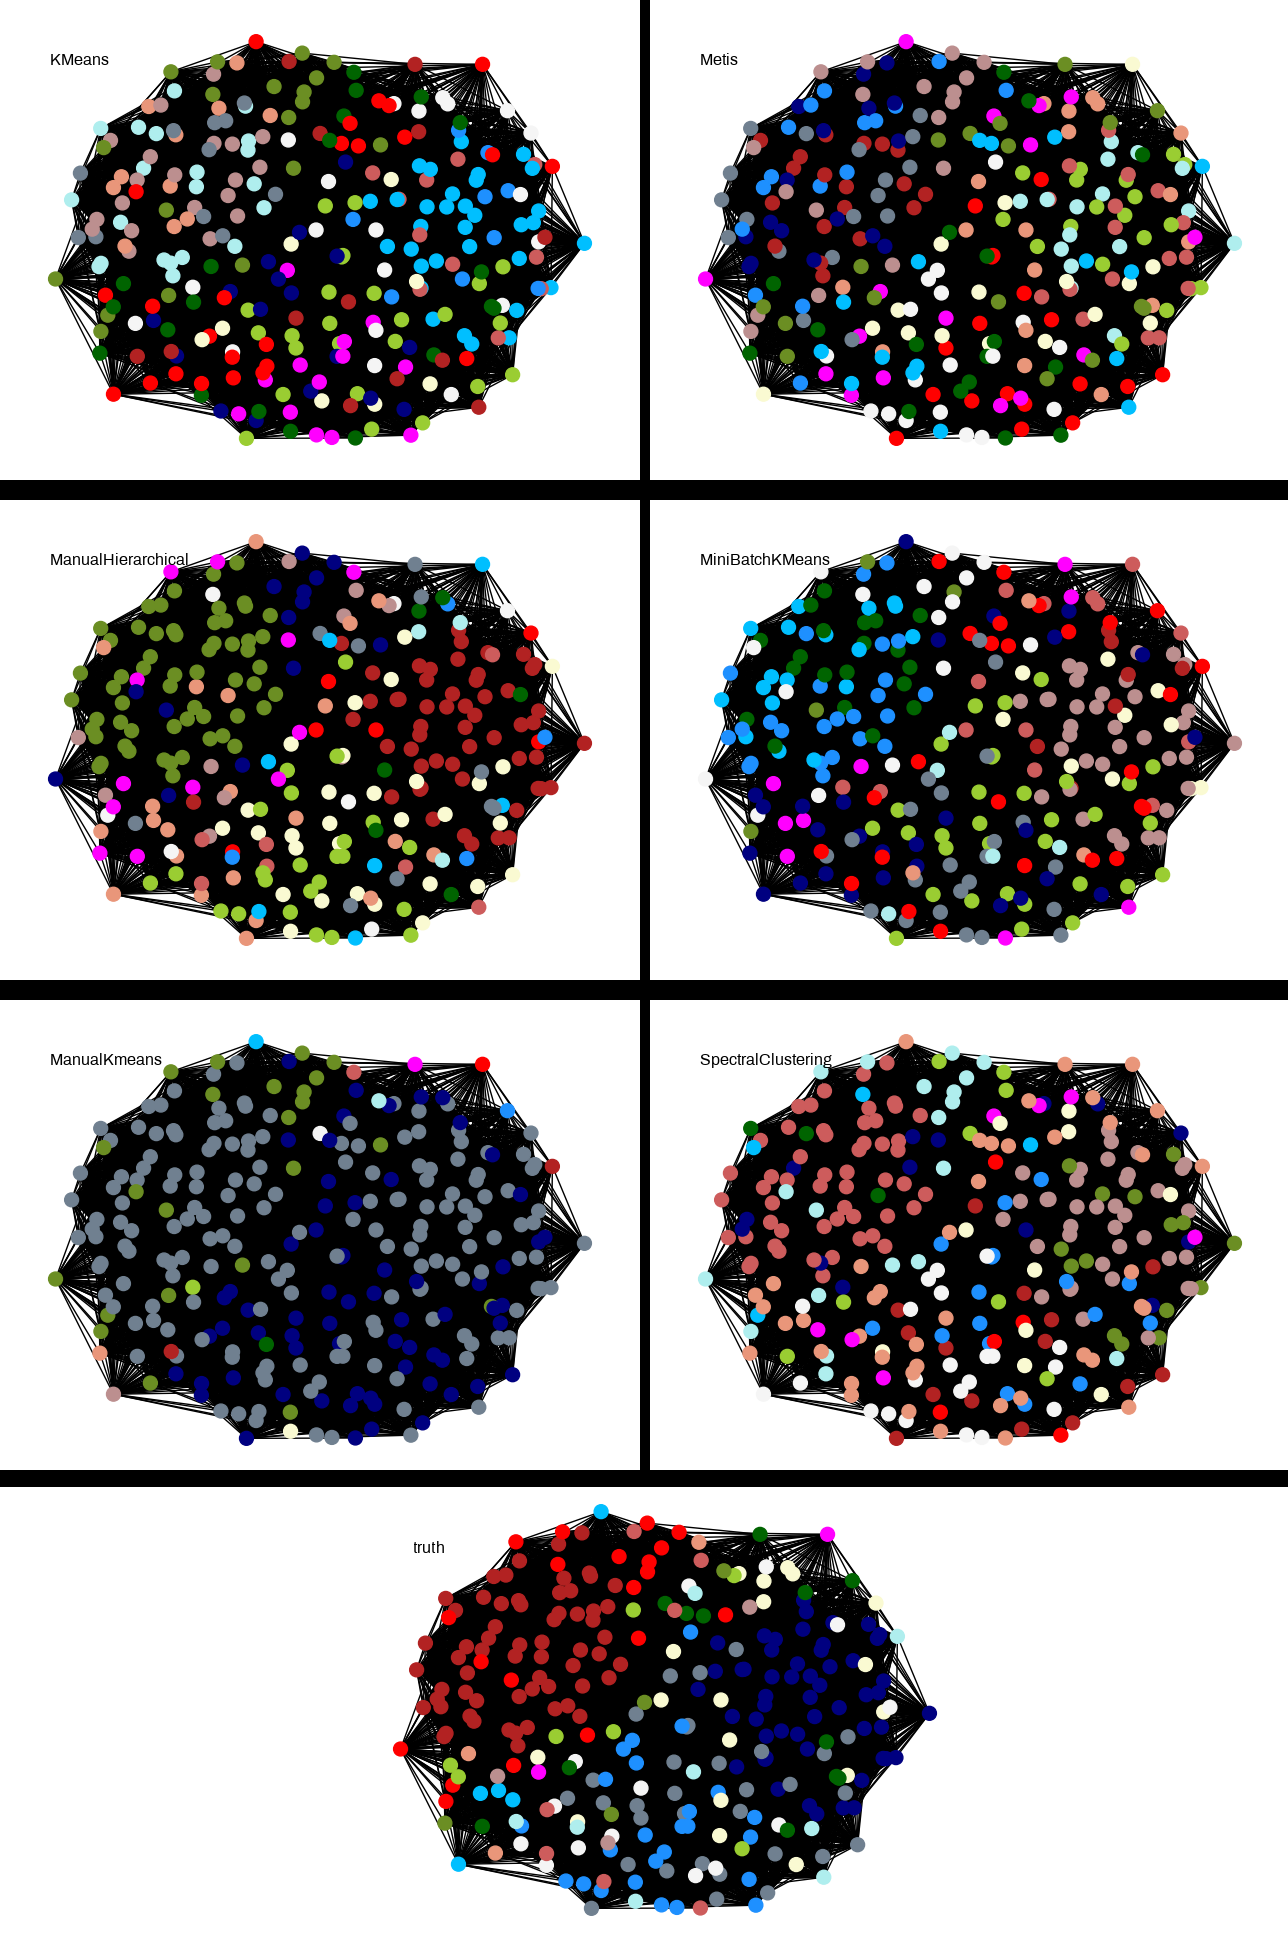
\includegraphics[width=.85\textwidth]{results/results_p-90_q-15.png}
    \caption[Clustering for $p=0.90,q=0.15$]{Results for $p=0.90,q=0.15$. Unfortunately, interpreting these results is more difficult than the previous due to the excess of edges present and lack of a natural method of laying out the vertices on a 2D plane.}
    \label{fig:results_p-90_q-15}
\end{figure}

\begin{figure}[H]
    \centering
    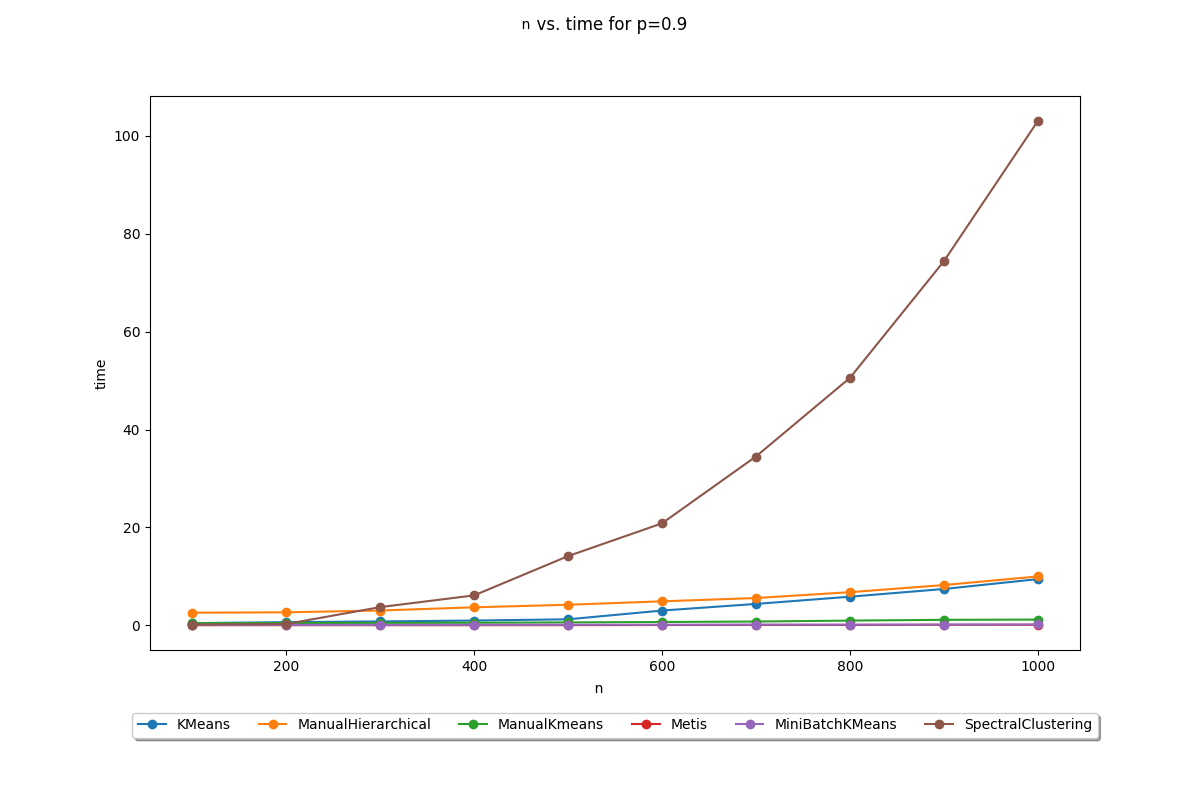
\includegraphics[width=.85\textwidth]{results/cluster_times.png}
    \caption[Clustering times across algorithms $p=0.90,q=0.20$]{Results for $p=0.90,q=0.15$ for various values of $n$. Specific trends are more fully discussed later, but there is a clear trend of more time consumed the larger the graph, though the computational complexity clearly differs across the algorithms.}
    \label{fig:cluster_times}
\end{figure}

\subsection{SBM Sparsification Results}

\begin{figure}[H]
    \centering
    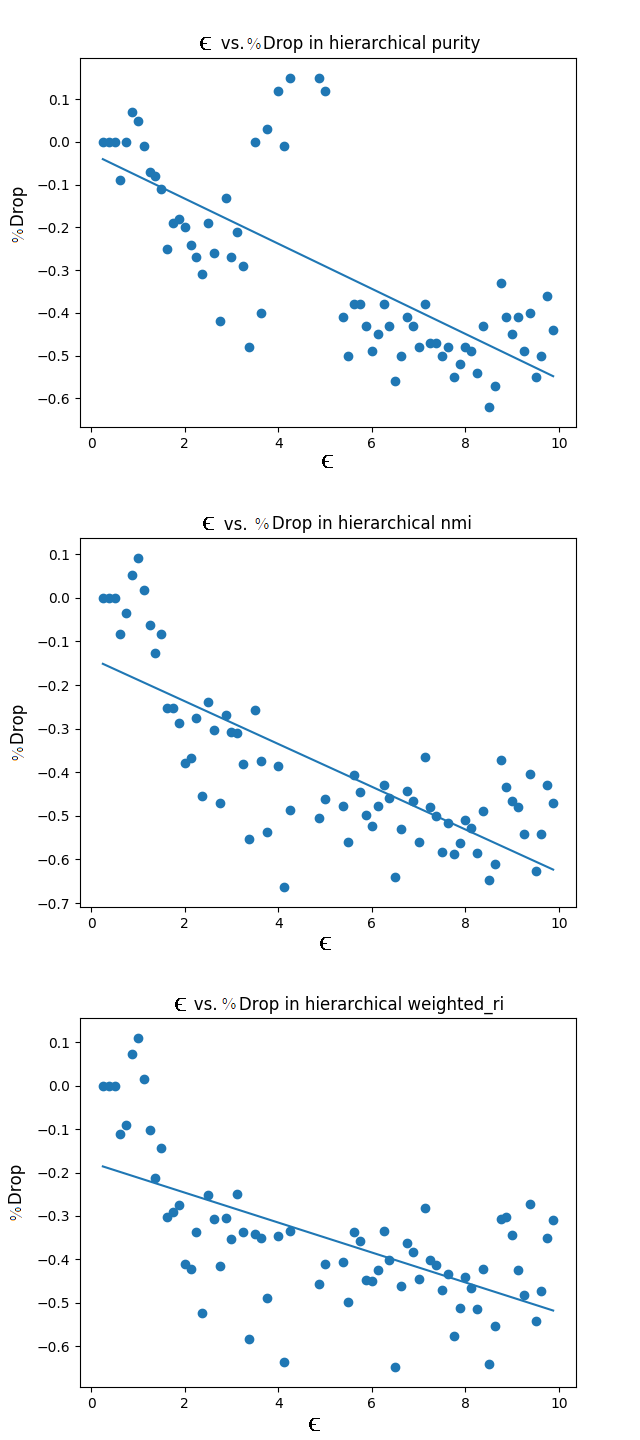
\includegraphics[width=.55\textwidth]{results/results_hierarchical_sparsify.png}
    \caption[Sparsified hierarchical spectral clustering for $p=0.75,q=0.10$]{For the fixed values of $p=0.75,q=0.10$, we performed sparsified hierarchical spectral clustering experiments, varying the $\epsilon$ parameter, as previously explained in Section \ref{sparsification-bg}. Note that the notation ``$\%_{drop}$" refers to the drop in the corresponding attribute as compared to a trial that was run without sparsification, meaning a value $<0$ refers to a drop in the corresponding metric.}
    \label{fig:results_hierarchical_sparsify}
\end{figure}

\begin{figure}[H]
    \centering
    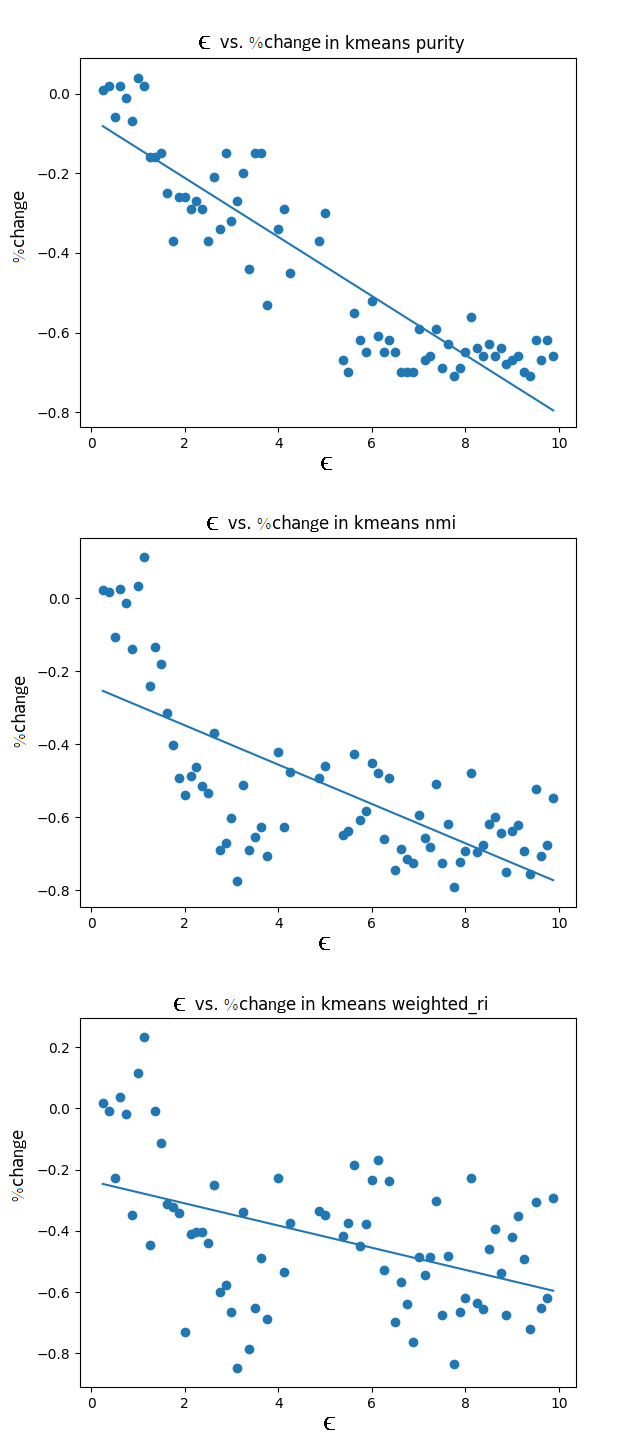
\includegraphics[width=.60\textwidth]{results/results_kmeans_sparsify.png}
    \caption[Sparsified k-means spectral clustering for $p=0.75,q=0.10$]{For the fixed values of $p=0.75,q=0.10$, we performed sparsified k-means hierarchical spectral clustering experiments, varying the $\epsilon$ parameter. A full explanation of the experiment can be found in the description of Figure \ref{fig:results_hierarchical_sparsify}.}
    \label{fig:results_kmeans_sparsify}
\end{figure}

\begin{figure}[H]
    \centering
    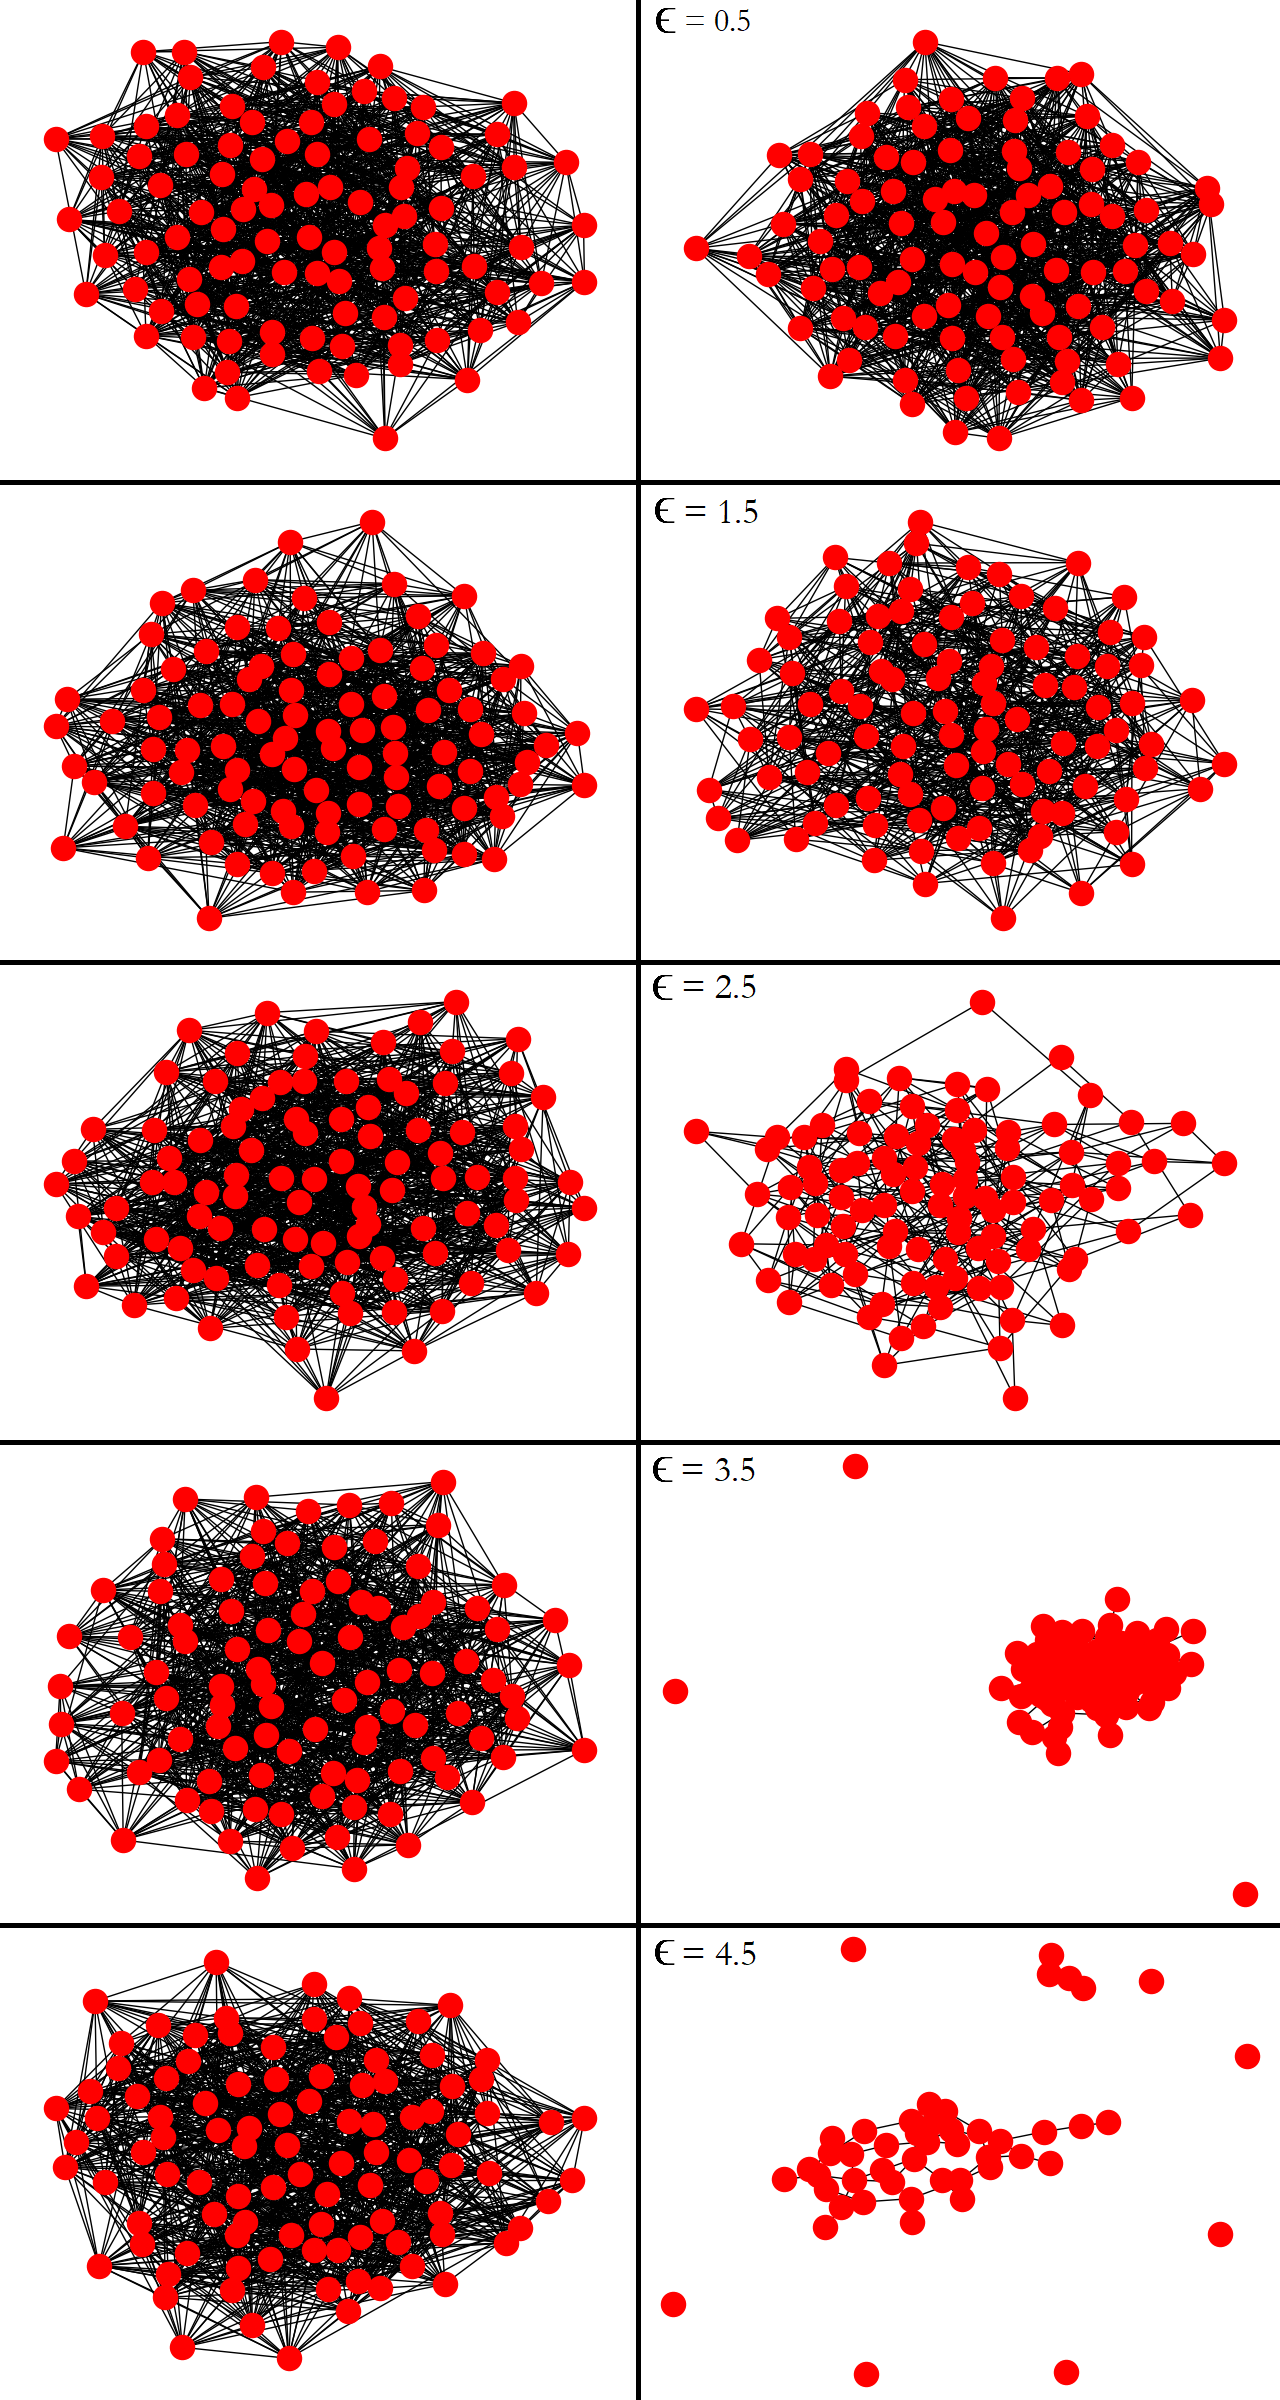
\includegraphics[width=.75\textwidth]{results/results_original_vs_sparse.png}
    \caption[Sparsified graphs across $\epsilon$]{For the original SBM with parameters $p=0.75,q=0.10$ on the left-hand side, these show the corresponding sparsified graphs, with parameters $\epsilon=0.5,1.5,2.5,3.5,4.5$ respectively following the graphs on the right-hand side. No clustering is depicted in this illustration, as it seeks to solely convey the extent to which edges were removed.}
    \label{fig:results_original_vs_sparse}
\end{figure}

\begin{figure}[H]
    \centering
    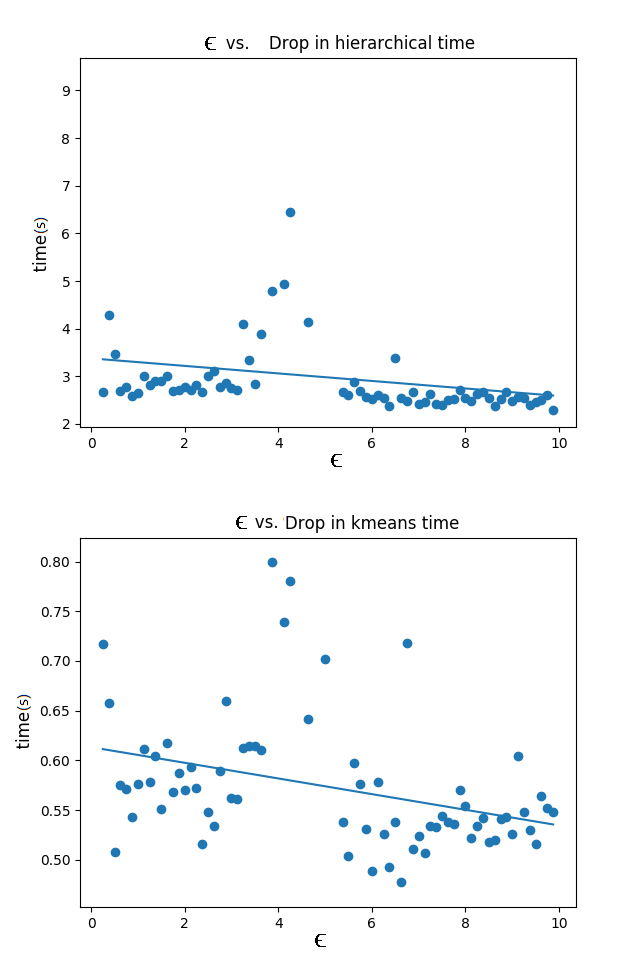
\includegraphics[width=.85\textwidth]{results/results_time_sparse.png}
    \caption[Clustering time vs. $\varepsilon$ sparsification parameter]{The time required for clustering with hierarchical (top) and k-means spectral clustering (bottom) with respect to the $\varepsilon$ sparsification parameter. Increasing $\varepsilon$ values correspond to a sparser graph. Surprisingly, there was no significant decrease in clustering time required even with increasing sparseness in the graph, more fully elaborated in the corresponding part of Section \ref{discussion}.}
    \label{fig:results_time_sparse}
\end{figure}

\subsection{SBM Coarsening Results}

\begin{figure}[H]
    \centering
    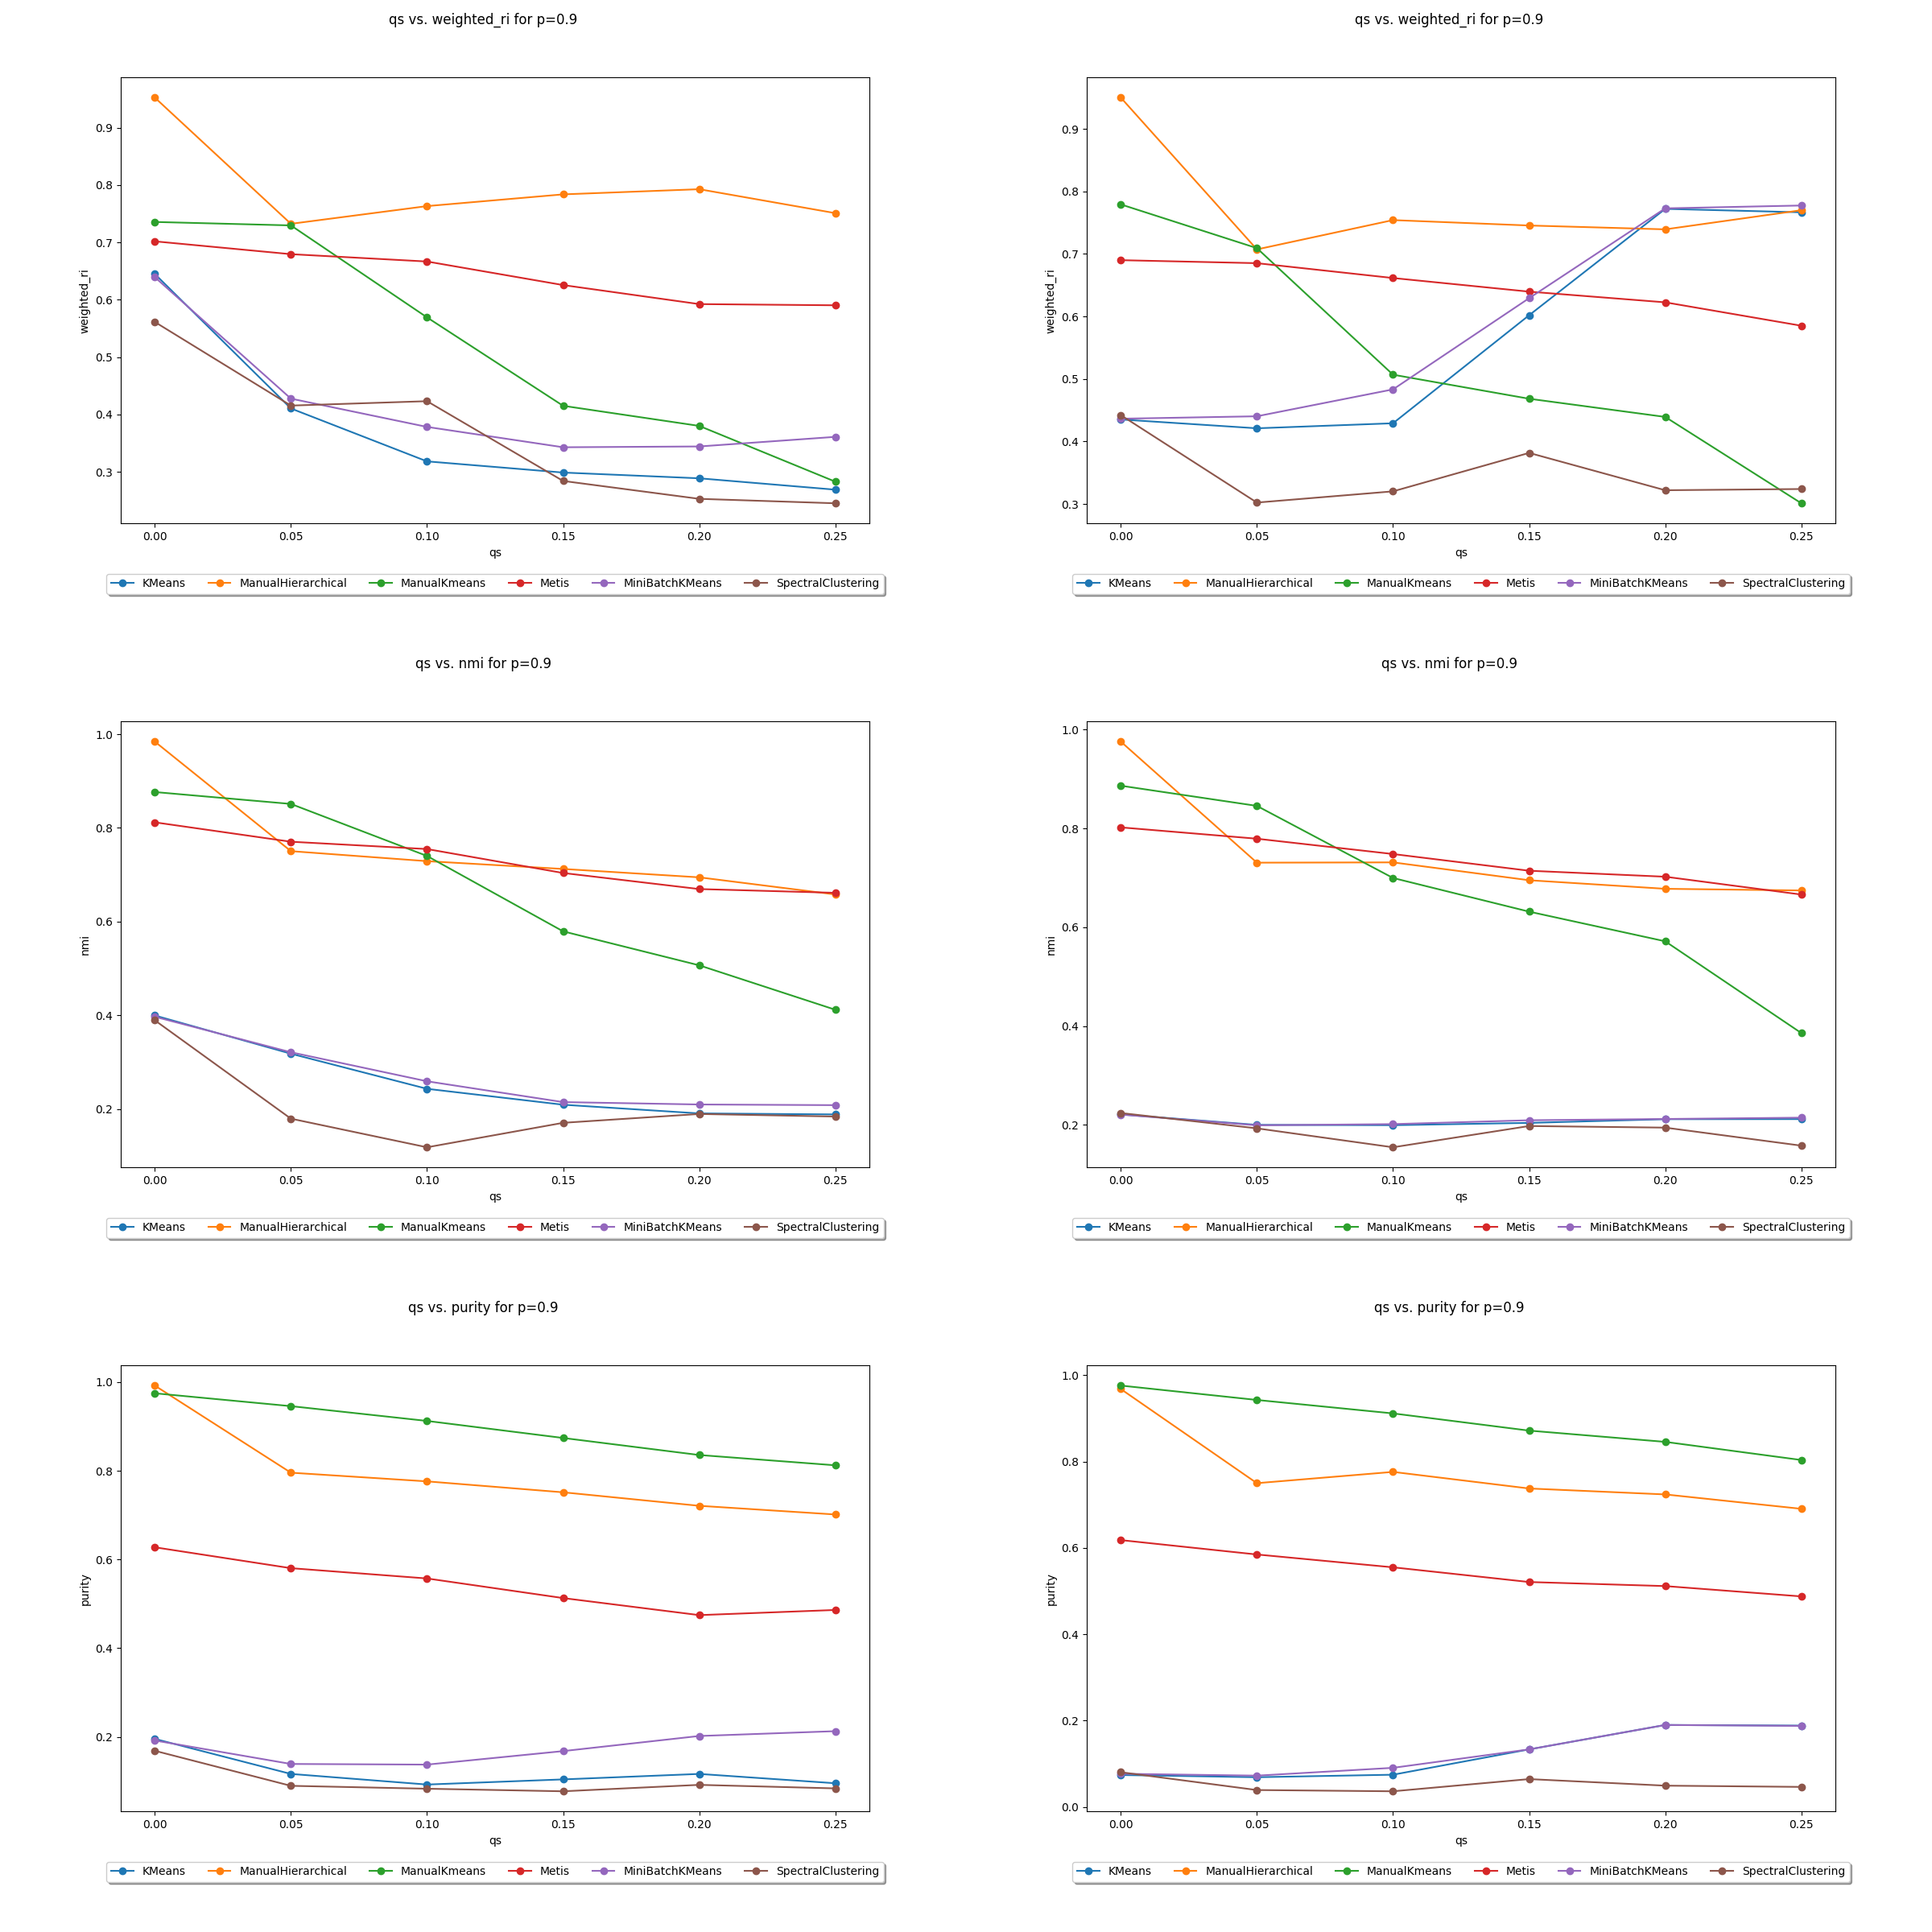
\includegraphics[width=1.0\textwidth]{results/results_coarsen.png}
    \caption[Coarsened accuracies across $p$]{Similar to the standard offline clustering algorithms, this shows (for the fixed choice of $p=0.9$) the variation of the different accuracy metrics over corresponding values of $q$. The left column is for \textbf{one} coarsening iteration; the right is for \textbf{two} iterations. METIS, while included for the sake of completeness, can be ignored for the purposes of discussion.}
    \label{fig:results_coarsen}
\end{figure}

\begin{figure}[H]
    \centering
    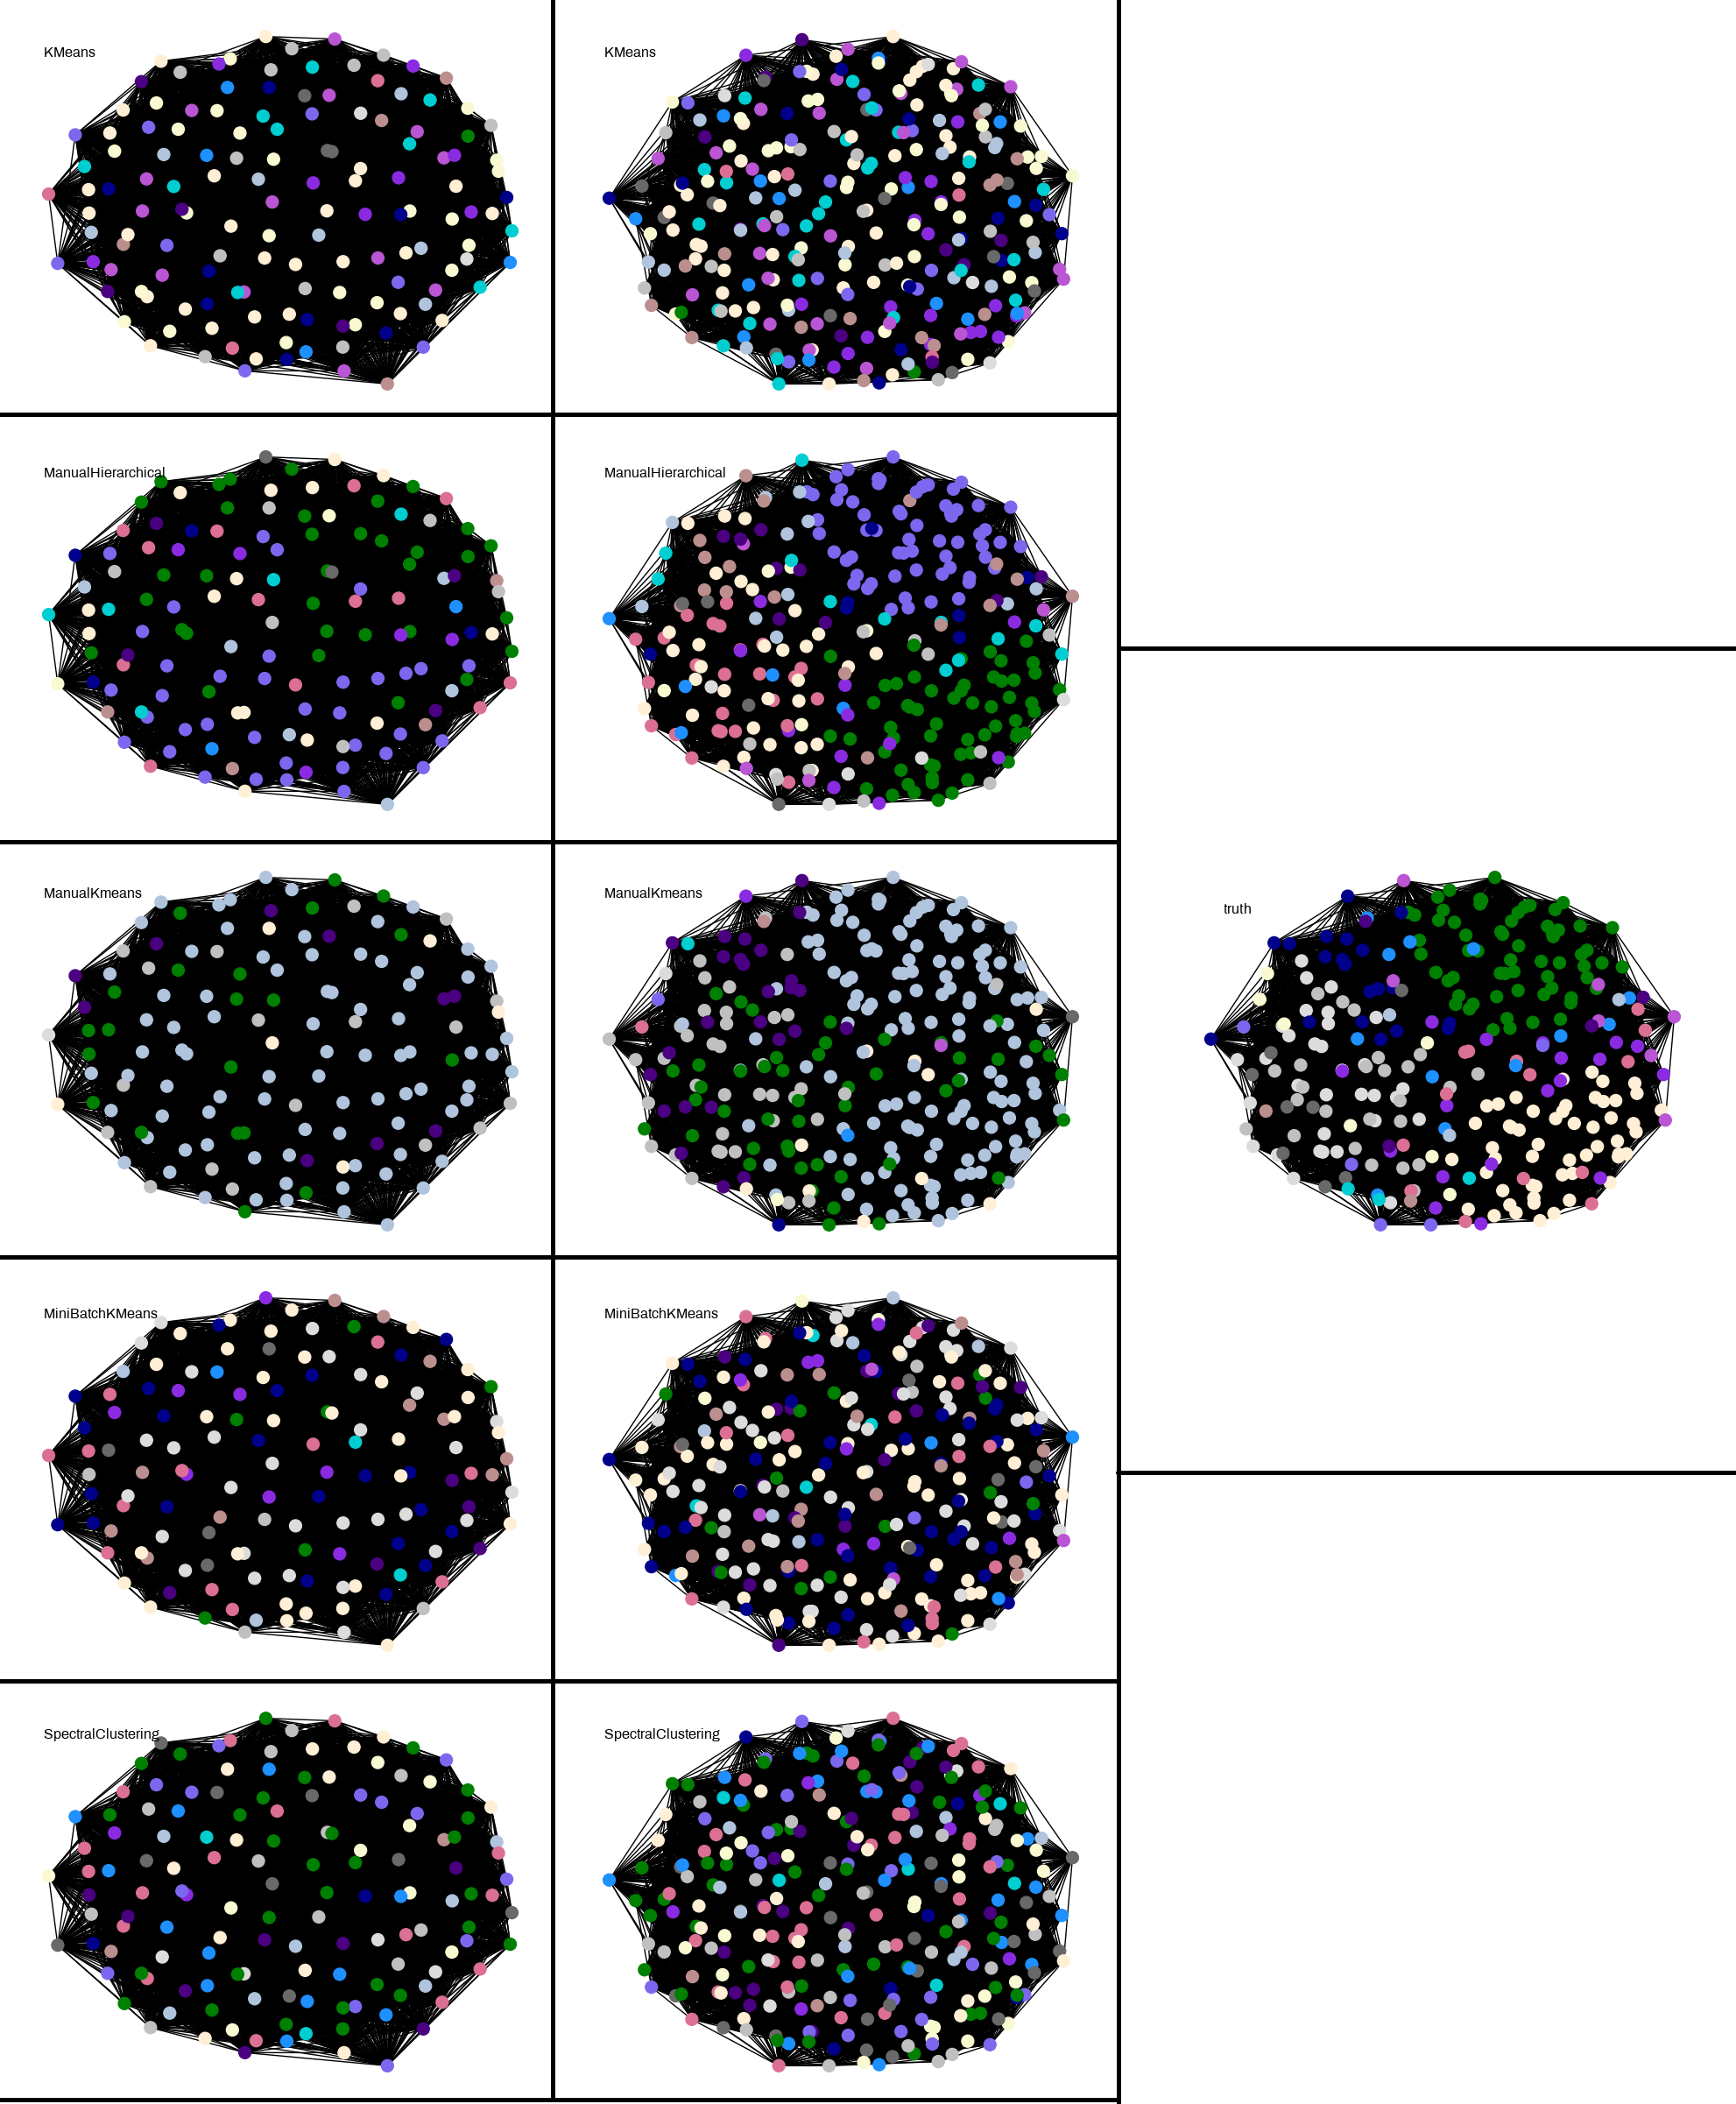
\includegraphics[width=1.0\textwidth]{results/results_contracted-1.png}
    \caption[Coarsened clustering for one iteration on $p=0.90,q=0.15$]{For the original underlying truth graph depicted on the far right, each of the left images depicts the clustering performed by various algorithms on the graph produced after \textit{one} iteration of coarsening, i.e. after one maximal matching was edge contracted and the corresponding expanded clustering to its right.}
    \label{fig:results_contracted-1}
\end{figure}

\begin{figure}[H]
    \centering
    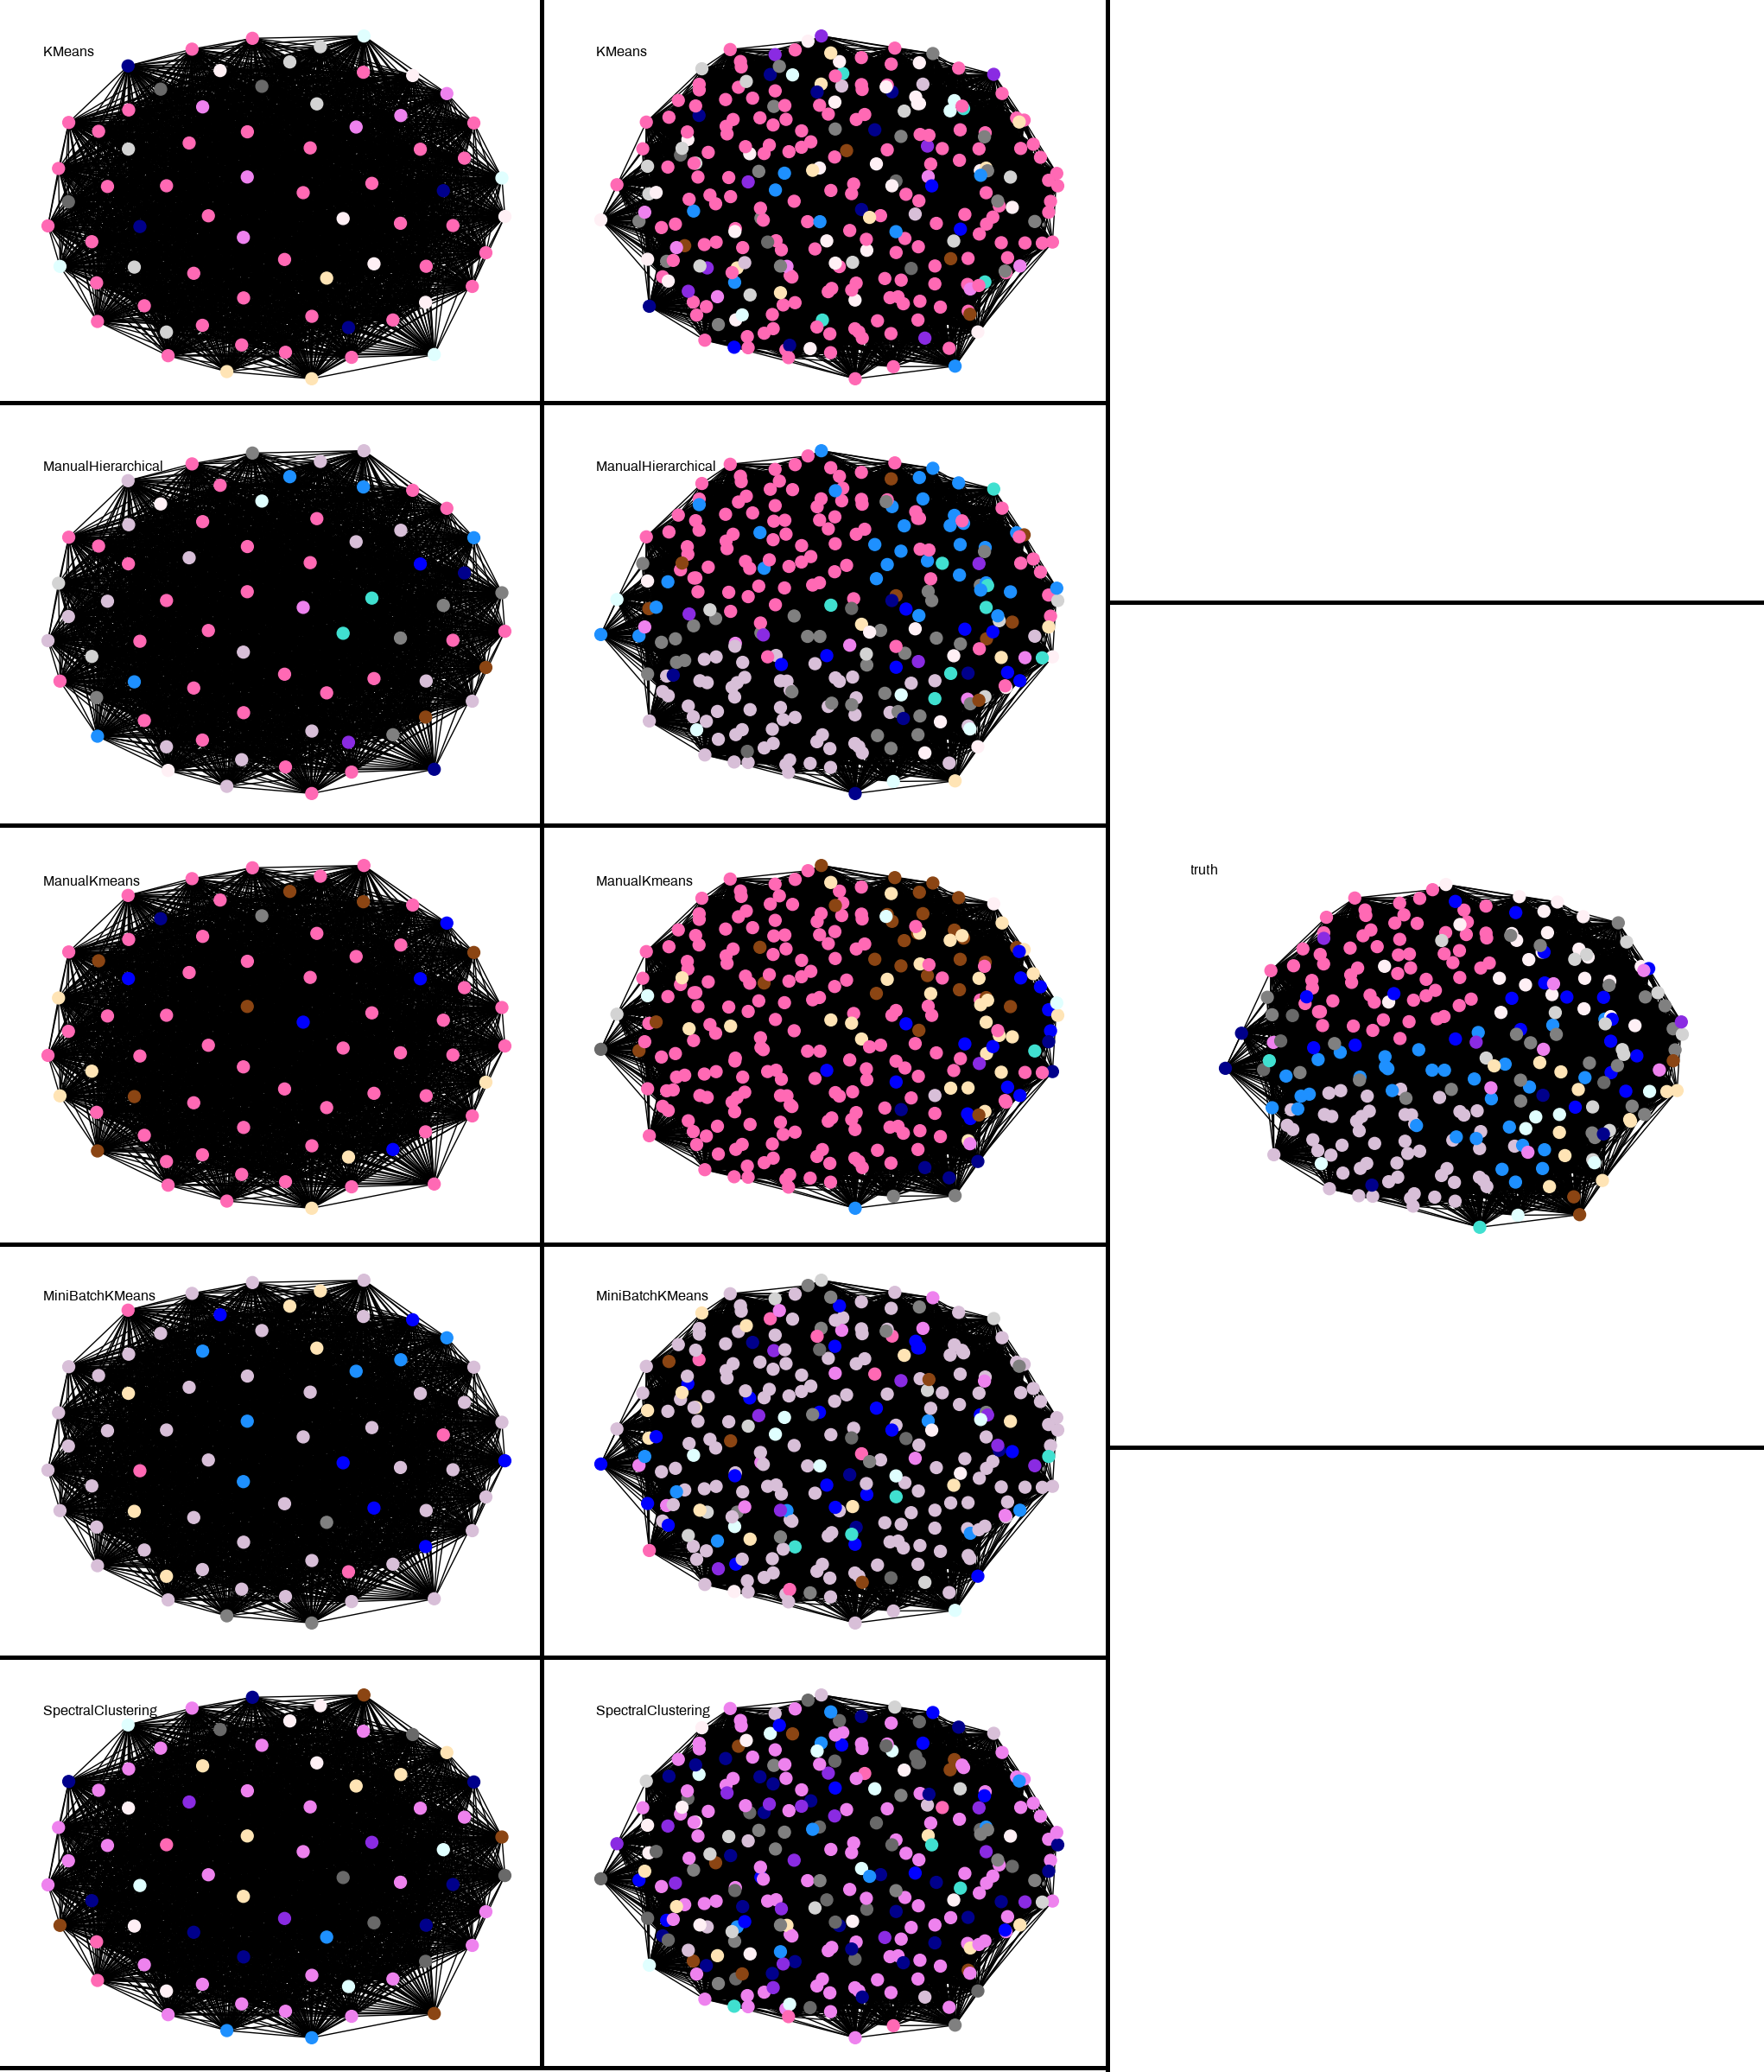
\includegraphics[width=1.0\textwidth]{results/results_contracted-2.png}
    \caption[Coarsened clustering for two iterations on $p=0.90,q=0.15$]{For the original underlying truth graph depicted on the far right, each of the left images depicts the clustering performed by various algorithms on the graph produced after \textit{two} iteration of coarsening, i.e. after two sets of maximal matchings were edge contracted and the corresponding expanded clustering to its right.}
    \label{fig:results_contracted-2}
\end{figure}

\begin{figure}[H]
    \centering
    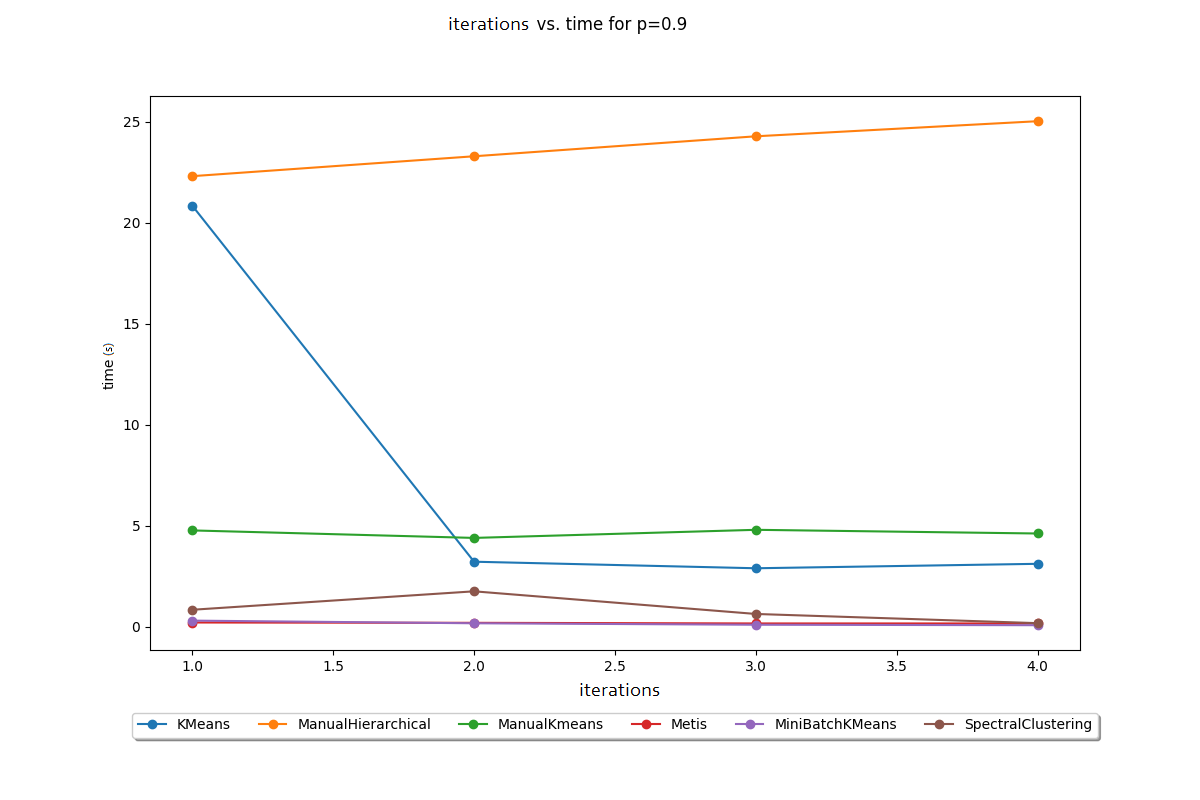
\includegraphics[width=1.0\textwidth]{results/results_coarsen_time.png}
    \caption[Clustering time vs. coarsening iterations]{As mentioned in the preceding descriptions, the iterations refers to how many sets of maximal matchings in the graph were contracted before the clustering was performed. Surprisingly, there was no significant decrease in clustering time required, as discussed in the corresponding part of Section \ref{discussion}.}
    \label{fig:results_coarsen_time}
\end{figure}

\subsection{SBM Online Results}

\subsection{Full Dataset Results}

\clearpage
\section{Discussion}\label{discussion}
As previously mentioned, the discussion of the results presented in the previous section are all below. 

\subsection{SBM Clustering Results}
From the results, we see many trends of importance in ascertaining the choice of clustering algorithm. As briefly mentioned previously, NMI was chosen to be the best metric of interest for our purposes. However, we first discuss each of the metrics in their own right, after which we discuss the overall results and the main choice of algorithm.

\subsubsection{Purity}
To begin the discussion, we look at the purity performance of these algorithms. Clearly, the spectral k-means clustering performed best with hierarchical spectral clustering similarly performing quite well. It is of note that these two algorithms were those that were implemented manually as compared to the performance of algorithms that came pre-developed in the \texttt{scikit-learn} package. Of course, this is with the caveat that the time performance was \textit{significantly} worse in the case of these two algorithms, as compared to the pre-developed counterparts, though that is discussed more thoroughly in the discussions that follow. The main reason k-means spectral clustering was particularly well performant here is likely because the eigenvectors were likely of the form discussed in Section \ref{spectral-bg}, namely where all the non-zero components for a given eigenvector corresponded to the same cluster. In other words, this implementation would prioritize keeping those associated vertices clustered together, whereas the hierarchical approach was indiscriminate in separating vertices in the progressive levels of division.

It is additionally of note to study the trend of algorithmic performance with respect to $p$ and $q$ alike, complemented with their sensitivities thereof. That is to say, as expected, all algorithms performed worse by this metric, as with all others, with increasing $q$. This is natural to assume, as, as $q\rightarrow p$, there is no way to differentiate, from the perspective of a single vertex, whether another is connected as a result of it being in the cluster or \textbf{not} being in the cluster. This trend, though visible, is less clearly present in the case of $p$. That is to say, for a given fixed value of $q$, observing the accuracy metric across various values of $p$ tended to show superior performance for high values of $p$, once again natural by the previous explanation.

In addition to these observation, it is quite noteworthy that METIS had \textit{very} little sensitivity to either of $p,q$. Specifically, while it tended to perform significantly worse on the easiest cases, i.e. for much of the lower values of $q$ for any given $p$, its relative performance tends to increase as $q$ increases. While nonintuitive, this aspect made METIS a compelling contender in addition to the manually implemented spectral clustering means, as most settings of graph clustering, particularly in our case, are not be nearly as well separated as in the simple cases where the standard algorithms were well-performant.

\subsubsection{NMI}
In addition to purity, we considered the NMI (normalized mutual information). Unlike the purity measure, the two most performant in this measure were the hierarchical spectral clustering and METIS algorithms. In fact, k-means spectral clustering performed worst in nearly all circumstances. This drastic difference in performance quality seems to suggest that k-means spectral clustering tended to over-compartmentalize the clustering. Specifically, this is because the intention of this metric was to address the issue of rewarding a clustering for assigning each vertex to its own cluster, which would perform well in the purity metric but not this. From this fact alone, choosing to continue with k-means spectral clustering offered additional problems that needed dealing with as compared to other algorithms.

Another surprising piece of performance was the relatively high accuracy of the simply k-means and partner mini-batch k-means algorithms for low values of $q$. In other words, for well separable data, k-means is perfectly well suited for the purpose of achieving high accuracy. In addition, given that k-means is such a widely implemented algorithm, its efficiency has been greatly optimized, as reflected in the time results discussed subsequently. Returning to the subject at hand, the geometric nature of k-means lends itself well to clustering well-separated data. Taking a step aside, the graphing algorithm itself, i.e. the force-based algorithm used to visualize/plot the graphs in NetworkX, serves as a spatial clustering algorithm. The case where the underlying clusters can be well separated in this visualization, therefore, mark circumstances where a well-developed spatial partitioning algorithm can be applied, which perfectly describes k-means. While not particularly applicable for the overall heuristics graph, this observation is useful potentially in analyzing subsets of the graph that separate well in visualization.

Further, this metric seems more sensitive to $q$ than was the purity. While still putting forth the same trend of diminishing value with $q\rightarrow\infty$, all algorithms \textit{except} hierarchical spectral clustering and METIS drastically diminish beyond $q=0.15$. Having said that, the consistency of these two algorithms make them appealing for the final heuristics graph use case, particularly as this is a setting where $q$ is not known and could greatly vary across different ``regions" in the graph.

\subsubsection{Weighted RI (F-score)}
From the weighted rand index (which specifically used $\beta=0.5$), there was not much additional information that could be gleaned that was not apparent from the NMI. Specifically, the hierarchical spectral clustering and METIS algorithms consistently perform best in the circumstances of higher $q$, whereas the simpler k-means family perform better in well-separated circumstances. The sensitivity of the F-score, however, is more comparable to that of purity with respect to $q$. The poor performance of k-means spectral clustering once again seems indicative of some form of overclustering behavior happening, since there seem to be many pairwise errors between vertices present even when the clusters themselves are quite pure.

\subsubsection{Time}
We first discuss the fully expected observations and then move on to the less obvious takeaways from this compilation. As previously mentioned, with the extensive use k-means finds in academia and industry alike, it has been greatly engineered and optimized in performance time. This, of course, comes bundled with the fact that its complementary mini-batch algorithm is more performant, as it only uses batches of the data to perform updates for the associated means, much in the way mini-batch gradient descent trades off time efficiency for accuracy. In addition to these notes, the general suite of \texttt{scikit-learn} algorithms all perform better than those developed manually. This should come as no surprise considering both the large community involved in the development of \texttt{scikit-learn}, its extensive industry use, and lack of thorough optimization considered in procuring the manual implementations of spectral clustering.

In addition to these obvious points of of consideration, however, was the point previously hypothesized of hierarchical spectral clustering performing generally better over accuracy metrics but worse in time compared to its k-means counterpart, which turned out to be true. As expected, the simultaneous clustering offered by k-means tends to separate vertices inappropriately top-down and misses key substructure that exists as a result of the disparate cluster sizes. Hierarchical clustering, in contrast, has ample opportunity to identify substructure, as each iteration looks to the existing clusters to determine which is ``most separable," meaning it only chooses to separate those clusters that naturally look at though they should be split. K-means has no such equivalent opportunity, meaning it works best in the case of there being similarly sized clusters across the true distribution. 

This k-means hiearchical clustering is additionally \textit{very} sensitive to small clusters. Namely, in the case of small clusters, a single ``dirty edge," i.e. presence of an edge when one should not exist or vice versa, would greatly throw off the corresponding eigenvector relative to the other eigenvectors. As a result, the corresponding eigenvalue would likely not be sufficiently close to 0 to be in the first $k$ eigenvectors, meaning it would completely ruin the prospect of clustering, whereas the comparable issue in hierarchical spectral clustering would solely soil a single ``leaf" in the tree of clustering bisections.

Having taken that aside, however, hiearchical clustering appears \textit{significantly} slower than all other clustering algorithms, which effectively renders it useless for the final application. That being said, however, ideally with further optimization and computation power, this algorithm could be brought to the point where it is applicable in such levels of scale. 

METIS, in contrast, performed \textit{significantly} faster than all other algorithms, pushing it as the ideal choice of use. Of course, this time efficiency likely arises from three sources. The first is one purely a matter of implementation, namely METIS is implemented in \texttt{C++} as compared to these other algorithms, which were developed in Python, though a majority tend to rely on \texttt{C++} API hooks rather than pure Python. The second is that METIS is written for parallel execution, that is, taking advantage of all cores present on the machine at hand. Unfortunately, Python has a global thread lock, making this less of a possibility for implementing such clustering efficiency improvements. The final point is that of the algorithm itself, which clearly works on a significantly reduced graph to improve time expended as compared to the vanilla algorithms, whose main bottleneck of eigendecomposition is approximately $O(n^3)$ for $n$ being the number of vertices involved. Thus, with these things considered, METIS was the clear choice in considering the time complexity.

\subsubsection{Overall}
From these overall weighted metrics, we therefore see the trends upon which we previously elaborated. Specifically, the family of k-means algorithms is well performant in the separable cases, whereas METIS and hierarchical spectral clustering perform better given a more heterogeneous graph. This is unfortunately obfuscated in the average performance graph. Namely, in averaging across the $q$ values, METIS seemingly much worse than it was in reality, owing to its poor performance on lower $q$ values. Thus, while the case of an \textit{average} $q$ seems to suggest k-means over METIS, this fully ignores the fact that we anticipate the heuristics graph to not be remotely well separated.

Taking a moment aside to elaborate on this crucial point, our graph, as previously mentioned, was catered with \textit{several} approximate heuristics. That is to say, many of the heuristics were explicitly placed such that, while they give \textit{some} suggestion about the link between two vertices, they are in no way fully indicative thereof. In other words, the graph was catered with the initial intention that a clustering algorithm would be capable of separating vertices with links between them if the associated heuristics were determined to not be strong or discriminatory enough. 

Having said that, it became necessary to prune clustering algorithms with the context of application in mind. In other words, as the k-means family is incapable of clustering tangled graphs, their applicability here was limited, despite their time efficiency being amongst the best offered by the alternatives. While this is the case herein, however, it may fully well be the case that future applications do not have such loosely catered heuristics and instead elect to use ones that are more definitive, as in ``Fistful of Bitcoin," in which case k-means would be a strongly recommended option.

In line with these points, therefore, the main options were either hierarchical spectral clustering or METIS. The former, however, from the time discussion was \textit{completely} impractical for the scale of graph considered herein. Thus, given the time constraints, METIS was the optimal choice for the purposes of this investigation, which carried forward against the alternative clustering techniques.

\subsection{SBM Sparsification Results}
As expected by definition of the spectral clustering parameter, we had greater sparsification happening as $\epsilon\rightarrow\infty$. In line with that, only the two spectral clustering algorithms were of relevance for this particular experiment, as this sparsification method was specifically chosen with the intention of procuring a graph whose Laplacian matrix was as similar to that of the original as possible, which is largely of relevance for spectral clustering. In addition, the spectral clustering of \texttt{scikit-learn} was not tested, as the previous section revealed that it consistently performed worse than either of the manually implemented alternatives by any of the metrics aside from time. 

Of note for the accuracy metrics is that the performance, which was expected to decline with increasing sparsification, due to the elimination of additional information, decreased seemingly piecewise. However, upon further investigation, it became clear that for certain levels of $\varepsilon$ (i.e. for sufficiently low values), no sparsification occurred, leaving the original graph. Similarly, for sufficiently high values, the entire graph simply consisted of separated vertices, making clustering an exercise in guessing. This explains the nature of there being two clumps of points near both the low and high values of $\varepsilon$ and a downward trend connecting the two clusters.

Surprisingly, however, the desired effect of time reduction was not too significant. It turns out that sparse matrices are not any easier to eigendecompose than their dense counterparts. Although there are more efficient means of calculating just the first few eigenvectors, rather than the entire decomposition, that arise in the case of sparse matrices, the original graph matrices were sufficiently sparse as to allow for that to be applied. In other words, sparsification offers little of service for our purpose, as the graph of 200 million vertices and 10 billion edges is roughly only $.000025\%$ filled with non-zero values. Hence, the main contender remained METIS without the implementation of additional sparsification at this point.

\subsection{SBM Coarsening Results}
As mentioned in the preceding exposition, discussion of METIS was moot for this particular setting. As it already includes coarsening, additional coarsening with worse reconstruction layered on top is impractical for future purposes, meaning there is little practical value to be gleaned from that analysis. Instead, we choose to investigate other trends. Of note is that all the non-manual performances were \textit{significantly} diminished in effectiveness as contrasted to the algorithms implemented manually. This perhaps has to do with the lesser sensitivity of the eigenvectors to the coarsening of the graph as compared to significant changes in spatial structure that arise from just collapsing a few nodes, explaining why k-means was affected detrimentally to such a large degree. This, however, fails to explain the significant drop in the performance of spectral clustering, for which a more thorough understanding of the source code would be required. Needless to say, the manual clustering fared relatively much better through degrees of coarsening.

Surprisingly, however, the coarsening did not provide ample speedup to warrant its integration. From the measured time performance, most of the algorithms were quite static across the number of iterations of coarsening. Each iteration, as it ``removes" a vertex, may remove many edges from the graph, as any incident edges would simply be integrated with those of the adjacency vertex. However, the supposed boost in speed would arise from the reduction in vertex count rather than that of edges, as evidenced by the lack of speedup from graph sparsification. Specifically, as eigendecomposition is $O(n^3)$, speed is greatly dependent upon the vertex count, meaning any significant reduction should greatly improve performance. 

However, it appears as though the process of obtaining a maximal matching itself takes up any time saved by this reduction, resulting in a relatively flat curve. It seems likely that METIS achieves its remarkable speed through use of parallel computation of matchings or simply a more optimized implementation thereof. From this, however, it seems that no manual coarsening can replace those performed in METIS, both due to the loss in efficiency and accuracy, resulting from the lack of corrections for projected partitions. Thus, from these results, we continue forward with the choice of METIS for clustering.

\subsection{SBM Online Results}

\subsection{Full Dataset Results}

\clearpage
\section{Conclusion}\label{conclusion}
Thus, from this investigation, we have found many points of interest for the deanonymization of Bitcoin and cryptocurrency transactions in general. Specifically, these points tend to deal with the general application of graph clustering algorithms towards the context of a catered heuristics graph associated with the likelihood two wallets correspond to the same real-world entity. Towards that end, we found that the family of k-means algorithms tend to be very well performant in both time and all accuracy metrics of interest when data is able to be spatially well separated. That is to say, with respect to the SBM, if the model at hand can be modelled for an arbitrary value of $p$ but low value of $q$, any k-mean derivative will be very suited. However, we found that the heuristics graph, which was quite loosely generated, did not have this desired spatial separability.

Given the non-flat geometries of clustering being sought, spectral clustering proved to have great performance. In particular, the hierarchical spectral methods had remarkable performance against all metrics but suffered greatly from a time efficiency perspective. K-means spectral clustering, on the other hand, suffered significant drawbacks on all accuracy metrics aside from purity, making it seem to be susceptible to over-compartmentalization in clustering. METIS, on the other hand, was \textit{significantly} faster than all other algorithms in performing clustering, though its relative performance on well-separated data was quite poor. METIS did have a level of consistency across the across all accuracy metrics when viewed across $q$ that made it an appealing choice for the purposes of clustering the full-scale graph.

In addition to these standard clustering algorithms, we attempted to performed sparsification, coarsening, and online clustering to see their relative performance in accuracy and time. Sparsification, however, caused both significant reductions in all accuracy metrics, across both k-means and hierarchical spectral clustering, without causing any significant reduction in time. We determined that no major improvements in clustering efficiency resulted from the removal of edges, as the eigendecomposition is largely independent of the presence of non-zero elements in the corresponding matrix. Coarsening, similarly, resulted in little reduction in time required for clustering and caused a reduction in efficiency, though this was more so caused by the time expended on performing the coarsening itself.

For the online clustering, we found \textbf{INSERT ONLINE RESULTS HERE}

From the final deanonymization, we found \textbf{INSERT FINAL RESULTS HERE}.

For future follow-on endeavors, there are some leads on what to investigate. The first revolves around the introduction of an automated weight updating algorithm on the heuristics. This would simply be based on some form of gradient descent updating on the weight. Much in the way SGD (stochastic gradient-descent) has currently become the de-facto means by which weights are updated in neural networks, this can be directly extended to the context of updating the weights associated with the heuristics based on its predictions on the set of vertices associated with the ground truth data. Initialization could be set uniformly or according to some appropriate random distribution.

A second line of interest revolves around the limitations of METIS. Specifically, as was found in many of the accuracy metrics, METIS is quite poorly performant for well-separable datasets. It, therefore, seems quite natural to pair METIS with a superior, similarly fast algorithm for such simple cases. Specifically, METIS would be best coupled with k-means for these circumstances. It follows that a method to determine the separability of data would need to be procured, from which a decision as to which algorithm to use could be made. Such a computation, however, would itself need to be made efficient should the overall algorithm be intended to be employed on the entire dataset. It, therefore, seems natural that this ``separability measurement" be done locally, akin to mini-batch.

In line with that, the hierarchical spectral clustering performed remarkably well by measure of all metrics yet could not be applied due to its being inefficient. In line with that, there arises the need to either look to parallelizing the algorithm or simply implement it in \texttt{C++} to see whether it could be applied to the generalized dataset and procure results of greater substance than were derived herein. Similarly, if the coarsening could be made more efficient, potentially by simply extracting the relevant code as it is implemented in METIS, it could be combined with hierarchical spectral clustering to procure a highly accurate and efficient method to be applied to the final dataset.

\clearpage
\singlespacing
\begin{thebibliography}{1}
\bibitem{data-stream} Aggarwal, Charu C., et al. ``A Framework for Clustering Evolving Data Streams." Proceedings 2003 VLDB Conference, 2003, pp. 81–92., doi:10.1016/b978-012722442-8/50016-1.
\bibitem{k-means} Arthur, David, and Sergei Vassilvitskii. ``k-Means++: The Advantages of Careful Seeding." \textit{Proceedings of the Eighteenth Annual ACM-SIAM Symposium on Discrete Algorithms}. Society for Industrial and Applied Mathematics, 2007. 
\bibitem{spectral-sparse} Batson, Joshua, et al. ``Spectral Sparsification of Graphs." Communications of the ACM, vol. 56, no. 8, 2013, p. 87., doi:10.1145/2492007.2492029.
\bibitem{coarsening} Chevalier, Cedric, and Ilya Safro. ``Comparison of Coarsening Schemes for Multilevel Graph Partitioning." Lecture Notes in Computer Science Learning and Intelligent Optimization, 2009, pp. 191–205., doi:10.1007/978-3-642-11169-3\_14.
\bibitem{evolutionary-temporal} Chi, Yun, et al. ``Evolutionary Spectral Clustering by Incorporating Temporal Smoothness." Proceedings of the 13th ACM SIGKDD International Conference on Knowledge Discovery and Data Mining - KDD '07, 2007, doi:10.1145/1281192.1281212.
\bibitem{silk} Christin, Nicolas. ``Traveling the Silk Road: A Measurement of a Large Anonymous Online Marketplace." 2012, doi:10.21236/ada579383.
\bibitem{scikit} ``Clustering." Scikit-Learn, scikit-learn.org/stable/modules/clustering.html.
\bibitem{coinjoin} ``CoinJoin: Bitcoin Privacy for the Real World." Bitcoin Talk, 22 Aug. 2013, bitcointalk.org/index.php?topic=279249.0.
\bibitem{dbscan} Daszykowski, M., and B. Walczak. ``Density-Based Clustering Methods." Comprehensive Chemometrics, 2009, pp. 635–654., doi:10.1016/b978-044452701-1.00067-3.
\bibitem{wiki-dbscan} ``DBSCAN." \textit{Wikipedia}, Wikimedia Foundation, 19 Apr. 2018, en.wikipedia.org/wiki/DBSCAN. 
\bibitem{eigen-update} Dhanjal, Charanpal, et al. ``Efficient Eigen-Updating for Spectral Graph Clustering." Neurocomputing, vol. 131, 2014, pp. 440–452., doi:10.1016/j.neucom.2013.11.015.
\bibitem{automatic} Ermilov, Dmitry, et al. ``Automatic Bitcoin Address Clustering." 2017 16th IEEE International Conference on Machine Learning and Applications (ICMLA), 2017, doi:10.1109/icmla.2017.0-118.
\bibitem{evaluation} ``Evaluation of Clustering." Stanford NLP, 2008, nlp.stanford.edu/IR-book/html/htmledition/evaluation-of-clustering-1.html.
\bibitem{follow} Greenberg, Andy. ``Follow The Bitcoins: How We Got Busted Buying Drugs On Silk Road's Black Market." Forbes, Forbes Magazine, 7 Sept. 2013, www.forbes.com/sites/andygreenberg/2013/09/05/follow-the-bitcoins-how-we-got-busted-buying-drugs-on-silk-roads-black-market/\#79bb83c8adf7.
\bibitem{bisection} Guattery, Stephen, and Gary L. Miller. ``On the Quality of Spectral Separators." \textit{SIAM Journal on Matrix Analysis and Applications}, vol. 19, no. 3, 1998, pp. 701–719., doi:10.1137/s0895479896312262. 
\bibitem{heuristics} ``Heuristics." \textit{BlockSci 0.4.5 Documentation}, citp.github.io/BlockSci/heuristics/heuristics.html. 
\bibitem{blocksci} Kalodner, Harry. ``BlockSci: Design and Applications of a Blockchain Analysis Platform." ArXiv Preprint, 2017, doi:1709.02489.
\bibitem{metis} Karypis, George, and Vipin Kumar. ``METIS--Unstructured Graph Partitioning and Sparse Matrix Ordering System, Version 2.0." 1995.
\bibitem{goldman} Katz, Lily. ``Goldman Says Cryptocurrencies May Succeed as Form of Real Money." Bloomberg.com, Bloomberg, 10 Jan. 2018, www.bloomberg.com/news/articles/2018-01-10/goldman-says-viability-of-crypto-is-highest-in-developing-world.
\bibitem{mincut} Kothari, Pravesh. ``Karger's Min Cut Algorithm." 2015, Princeton University, Princeton University.
\bibitem{dynamic} LaViers, Amy, et al. ``Dynamic Spectral Clustering." Georgia Institute of Technology, 2010.
\bibitem{sketch} Liberty, Edo. ``Simple and Deterministic Matrix Sketching." Proceedings of the 19th ACM SIGKDD International Conference on Knowledge Discovery and Data Mining - KDD '13, 2013, doi:10.1145/2487575.2487623.
\bibitem{spectral} Luxburg, Ulrike Von. ``A Tutorial on Spectral Clustering." Statistics and Computing, vol. 17, no. 4, 2007, pp. 395–416., doi:10.1007/s11222-007-9033-z.
\bibitem{fistful} Meiklejohn, Sarah, et al. ``A Fistful of Bitcoins." Proceedings of the 2013 Conference on Internet Measurement Conference - IMC '13, 2013, doi:10.1145/2504730.2504747.
\bibitem{laundering} Moser, Malte, et al. ``An Inquiry into Money Laundering Tools in the Bitcoin Ecosystem." 2013 APWG ECrime Researchers Summit, 2013, doi:10.1109/ecrs.2013.6805780.
\bibitem{sbm} Mossel, Elchanan, et al. ``Reconstruction and Estimation in the Planted Partition Model." Probability Theory and Related Fields, vol. 162, no. 3-4, 2014, pp. 431–461., doi:10.1007/s00440-014-0576-6.
\bibitem{bitcoin} Nakamoto, Satoshi. ``Bitcoin: A Peer-to-Peer Electronic Cash System." 2008.
\bibitem{incremental} Ning, Huazhong, et al. ``Incremental Spectral Clustering by Efficiently Updating the Eigen-System." Pattern Recognition, vol. 43, no. 1, 2010, pp. 113–127., doi:10.1016/j.patcog.2009.06.001.
\bibitem{dynamic-sbm} Pensky, Marianna, and Teng Zhang. ``Spectral Clustering in the Dynamic Stochastic Block Model." ArXiv Preprint, 2017, doi:1705.01204.
\bibitem{fast-coarsen} Purohit, Manish, et al. ``Fast Influence-Based Coarsening for Large Networks." Proceedings of the 20th ACM SIGKDD International Conference on Knowledge Discovery and Data Mining - KDD '14, 2014, doi:10.1145/2623330.2623701.
\bibitem{spectral-bisection} Rocha, Israel. ``Improvements on Spectral Bisection." ArXiv Preprint, 2017, doi:1703.00268.
\bibitem{cluster-review} Schaeffer, Satu Elisa. ``Graph Clustering." Computer Science Review , 2007, pp. 27–64.
\bibitem{bitcoin-etf} ``Self - Regulatory Organizations; NYSE Arca, Inc; Order Instituting Proceedings to Determine Whether to Approve or Disapprove a Proposed Rule Change to List and Trade the Shares of the ProShares Bitcoin ETF and the ProShares Short Bitcoin ETF under NYSE Arca Rule 8.200 - E, Commentary .02." Securities and Exchange Commission, 23 Mar. 2018.
\bibitem{fast-kmeans} Shindler, Michael, et al. ``Fast and Accurate k-Means For Large Datasets.” Advances in Neural Information Processing Systems, 2011. 
\bibitem{public-key} Shirriff, Ken. ``Ken Shirriff's Blog." Bitcoins the Hard Way: Using the Raw Bitcoin Protocol, www.righto.com/2014/02/bitcoins-hard-way-using-raw-bitcoin.html. 
\bibitem{resistance} Spielman, Daniel A., and Nikhil Srivastava. ``Graph Sparsification by Effective Resistances." Proceedings of the Fourtieth Annual ACM Symposium on Theory of Computing - STOC 08, 2008, doi:10.1145/1374376.1374456.
\bibitem{graph-viz} Tamassia, Roberto. Handbook of Graph Drawing and Visualization. CRC Press Taylor \& Francis Group, 2016. 
\bibitem{terry} Tao, Terrence. ``A Review of Probability Theory." \textit{Terry Tao}, terrytao.wordpress.com/2010/01/01/254a-notes-0-a-review-of-probability-theory/.
\bibitem{virtual} Trautman, Lawrence J. ``Virtual Currencies: Bitcoin \& What Now after Liberty Reserve and Silk Road?" SSRN Electronic Journal, 2014, doi:10.2139/ssrn.2393537.
\bibitem{blockchain-img} Wander, Matthaus. ``Bitcoin Block Data." Wikimedia Commons, 22 June 2013, commons.wikimedia.org/wiki/File:Bitcoin\_Block\_Data.png.
\bibitem{scalable} Whang, Joyce Jiyoung, et al. ``Scalable and Memory-Efficient Clustering of Large-Scale Social Networks." 2012 IEEE 12th International Conference on Data Mining, 2012, doi:10.1109/icdm.2012.148.
\bibitem{streaming} Yoo, Shinjae, et al. “Streaming Spectral Clustering.” 2016 IEEE 32nd International Conference on Data Engineering (ICDE), 2016, doi:10.1109/icde.2016.7498277. 
\bibitem{ico} Zetzsche, Dirk A., et al. ``The ICO Gold Rush: It's a Scam, It's a Bubble, It's a Super Challenge for Regulators." SSRN Electronic Journal, 2017, doi:10.2139/ssrn.3072298.
\end{thebibliography}

\clearpage
\section*{Honor Pledge}
\textit{I pledge my honour that this paper represents my own work in accordance with University regulations.}

\noindent - Yash Patel

\end{document}